\documentclass{article}

\usepackage[utf8]{inputenc}
\usepackage{amssymb}
\usepackage{amsmath}
\usepackage{amsthm}
\usepackage{amsfonts}
\usepackage{float}
\usepackage{tikz}
\usepackage{subcaption}

\usetikzlibrary{calc,decorations.markings,positioning,shapes,patterns, intersections,matrix,decorations.pathreplacing,quotes}

 \newcommand{\I}{\mathcal{I}}
 \newcommand{\Lmax}{L_{\max}}
 \newcommand{\RR}{\mathcal{R}}
 \newcommand{\DT}{\frac{d}{dt}}

 \newcommand{\DDE}{\frac{D}{d\eta}}

 \newcommand{\DI}{\partial^I}
 \newcommand{\DE}{\partial_{\eta}}
 \newcommand{\NDV}{\frac{\partial_{v}}{R}}
 \newcommand{\NDU}{\frac{\partial_{u}}{R}}
 \newcommand{\DUV}{\partial_{uv}}
 \newcommand{\DUU}{\partial_{uu}}
 \newcommand{\DVV}{\partial_{vv}}

 \newcommand{\argmin}{\operatornamewithlimits{argmin}}
\newcommand{\argmax}{\operatornamewithlimits{argmax}}

 \newcommand{\Ae}{\text{a.e. }}
 \newcommand{\Csurf}{C_{\text{surf }}}
 \newcommand{\ForAe}{\text{for a.e. }}
 \newcommand{\PLH}{{\mkern-1mu\times\mkern-1mu}}
 \newcommand{\Times}{\PLH}

 \renewcommand{\i}{\mathrm{i}}
\newcommand{\C}{\mathbb{C}}
\newcommand{\R}{\mathbb{R}}
\newcommand{\A}{\mathcal{A}}
\newcommand{\Z}{\mathbb{Z}}
\newcommand{\surf}{M}
\newcommand{\EN}{\mathbb{N}}
\newcommand{\ko}{\kappa}
\newcommand{\kop}{\kappa^{\mathrm{map}}}

\newcommand{\DU}{\partial_{u}}
\newcommand{\DV}{\partial_{v}}
\newcommand{\DerU}{\partial_{u}}
\newcommand{\DerV}{\partial_{v}}
\newcommand{\DerUV}{\partial^2_{uv}}
\newcommand{\DerUU}{\partial^2_{uu}}
\newcommand{\DerVV}{\partial^2_{vv}}

\newcommand{\du}{\mathrm{d}u}
\newcommand{\dx}{\mathrm{d}x}
\newcommand{\dv}{\mathrm{d}v}
\newcommand{\dr}{\mathrm{d}r}
\newcommand{\ds}{\mathrm{d}s}
\newcommand{\dt}{\mathrm{d}t}
\newcommand{\dl}{\mathrm{d}l}
\newcommand{\dz}{\mathrm{d}z}
\newcommand{\modif}[1]{\textcolor{red}{#1}}

\newcommand{\J}{\mathcal{J}}

\newcommand{\psileft}{\psi^{\text{left}}}
\newcommand{\psiright}{\psi^{\text{right}}}
\newcommand{\sect}{Q}
\newcommand{\HalfP}{S}
\newcommand{\halfP}{B}
\newcommand{\cjunc}{\eta_{\text{junc}}}
\newcommand{\koin}{\ko_{\text{init}}}
\newcommand{\OO}{\mathcal{O}}
\newcommand{\psim}{|\psi|_{l^\infty}}
\newcommand{\psitot}{|\psi|_{l^1}}
\newcommand{\hmax}{h_{\max}}
\newcommand{\hmin}{h_{\min}}
\newcommand{\N}{\mathcal{N}}
\renewcommand{\S}{\mathcal{S}}
\renewcommand{\O}{\mathcal{O}}
\newcommand{\U}{\mathcal{U}}
\newcommand{\V}{\mathcal{V}}
\newcommand{\Nsing}{\mathcal{N}_{\mathrm{sing}}}
\newcommand{\Nver}{\mathcal{N}_{\mathrm{ver}}}
\newcommand{\Ned}{\mathcal{N}_{\mathrm{ed}}}
\newcommand{\Ndel}{\mathbf{N}}
\newcommand{\ndel}{\mathbf{n}}
\newcommand{\Npiece}{\mathcal{N}_{\mathrm{piece}}}
\newcommand{\phiband}{\varphi_{\mathrm{band}}}
\newcommand{\Bcband}{B_c^{\mathrm{band}}}
\newcommand{\Beband}{B_e^{\mathrm{band}}}
\newcommand{\NpolT}{\tilde{\mathcal{N}}_{\mathrm{pol}}}
\newcommand{\NpieceT}{\tilde{\mathcal{N}}_{\mathrm{piece}}}



\renewcommand{\H}{\mathcal{H}}
\newcommand{\Npol}{\mathcal{N}_{\mathrm{pol}}}

\newtheorem{theorem}{Theorem}
\newtheorem{lemma}[theorem]{Lemma}
\newtheorem{proposition}[theorem]{Proposition}
\newtheorem{corollaryF}[theorem]{Corollaire}
\newtheorem{definitionF}[theorem]{D�finition}

\newtheorem{conjecture}[theorem]{Conjecture}
\newtheorem{proprieteE}[theorem]{Property}
\newtheorem{problematiqueE}[theorem]{Issue}
\newtheorem{questionE}[theorem]{Question}
\newtheorem{corollaryE}[theorem]{Corollary}
\newtheorem{definitionE}[theorem]{Definition}

\theoremstyle{remark}
\newtheorem{exempleE}[theorem]{Example}
\newtheorem{remarkE}[theorem]{Remark}
\newtheorem{exempleF}[theorem]{Exemple}
\newtheorem{remarkF}[theorem]{Remarque}


\newtheoremstyle{prpart}% name of the style to be used
  {\topsep}% measure of space to leave above the theorem. E.g.: 3pt
  {\topsep}% measure of space to leave below the theorem. E.g.: 3pt
  {}% name of font to use in the body of the theorem
  {0pt}% measure of space to indent
  {}% name of head font
  {. }% punctuation between head and body
  { }% space after theorem head; " " = normal interword space
  {\textbf{\thmname{#1} \thmnumber{#2}}\textit{\thmnote{ (#3)}}}
  
\theoremstyle{prpart}
\newtheorem{proofpart}{Step}

\makeatletter
\@addtoreset{proofpart}{theorem}
\makeatother

\makeatletter
\long\def\my@drawfill#1#2;{%
\@skipfalse
\fill[#1,draw=none] #2;
\@skiptrue
\draw[#1,fill=none] #2;
}

\newcommand{\drawfill}[1][]{%
  \my@drawfill{#1}}

\newif\if@skip

\newcommand{\skipit}[1]{%
\if@skip
\else
#1
\fi
}

\newcommand{\comment}[1]{}

\newcommand{\CC}{\mathcal{C}}
\renewcommand{\H}{\mathcal{H}}
\newcommand{\B}{\mathcal{B}}
\newcommand*{\Scale}[2][4]{\scalebox{#1}{$#2$}}%

\newcommand{\snum}{\addtocounter{equation}{1}\tag{\theequation}}

 \newcommand{\PU}{\partial_{u}\varphi}
 \newcommand{\PV}{\partial_{v}\varphi}
 \newcommand{\NPU}{{\textstyle\frac{\partial_{u}\varphi}{R}}}

 \newcommand{\Id}{\mathrm{Id}}
\newcommand{\ind}{\mathrm{Ind}}
\newcommand{\hol}{\mathrm{Hol}}
\newcommand{\etaI}{\eta_{\mathrm{set}}}
\newcommand{\gammaI}{\gamma_{\mathrm{set}}}
\newcommand{\st}{g}
\newcommand{\pt}{p}

\begin{document}

\title{Construction of Chebyshev nets with singularities}
\maketitle

\begin{center}{Y.~Masson$^{\textrm{1}}$,
    A.~Ern$^{\textrm{1}}$, L.~Hauswirth$^{\textrm{2}}$,
    L.~Monasse$^{\textrm{1}}$} \end{center}
\begin{center}
  $^{\textrm{1}}$ Universit\'e Paris-Est, CERMICS (ENPC), \\
  6 et 8 avenue Blaise Pascal, Cit\'e Descartes, Champs sur Marne, 77455, Marne la Vall\'ee, Cedex 2, France.
\end{center}
\begin{center}
  $^{\textrm{2}}$ Universit\'e Paris-Est, LAMA, \\
  5 boulevard Descartes, Cit\'e Descartes, Champs sur Marne, 77455, Marne la Vall\'ee, Cedex 2, France.
\end{center}

\bibliographystyle{plain}

\textcolor{red}{DEBUT DU CHAPITRE 4}
 

\section{Introduction}

\textcolor{red}{A FAIRE !!!}

 

 
 
 We prove in this chapter the existence and the uniqueness of a Chebyshev net delimited by two smooth curves called boundary conditions. We outline the main ideas of the proof as follows. Following \cite{Ghys09}, we consider the angle distribution defined by the angle between the coordinate curves of the candidate Chebyshev net. We prove that one can construct a unique mapping from this angle distribution such that the $v$-coordinate curves are arc-length parametrized curves with the proper geodesic curvature defined by this angle distribution. Note that the choice of the direction is arbitrary, so that the $u$-coordinate curves could have been chosen. This construction entails a loss of symmetry between these two coordinates which materializes itself by a differentiation between the regularity of the two directions of coordinates curves. The aim is now to view the Hazzidakis formula as a fixed-point equation on the angle distribution, using that the candidate Chebyshev net depends (Lipschitz) continuously on this angle distribution. 

 We then show that, supposing that the Hazzidakis formula is satisfied by the angle distribution, we obtain a regularity pick-up by the use of this identity, and therefore we recover the symmetry between the two directions. Furthermore, we prove that, under suitable regularity conditions, the candidate mapping constructed from the angle distribution is indeed a Chebyshev net, i.e., the $u$-coordinate curves are also arc-length parametrized. The last step of the proof is to show the existence of a unique solution to the equation associated with Hazzidakis formula. This is obtained in the spirit of the Cauchy--Lipschitz theorem: we first prove this existence and uniqueness for a small interval in the $v$-coordinate, and we then extend this result to the whole domain.


\section{Preliminaries}
\subsection{Informal statement of the main result}
Let 
\begin{equation*}
  D=[0,L_u]\Times[0,L_v],\quad\text{with } L_u,L_v\in\R_\ast^+,
\end{equation*}
 and let $\gamma_u:[0,L_u]\to\surf$ and $\gamma_v:[0,L_v]\to\surf$ be two curves such that $\gamma_u(0)=\gamma_v(0)$, and forming an interior angle $\angle(\gamma_u'(0),\gamma_v'(0))\in(0,\pi)$ at their intersection. For clarity of exposition, throughout this chapter, we consider a slightly different notion of Chebyshev net which will refer to mappings (not necessarily homeomorphisms) $\varphi:D\to\surf$ satisfying
\begin{subequations}\label{eq:cheb-def-c3}
\begin{align}\label{eq:cheb-def-c3a}
|\partial_u \varphi|_g(u,v) = 1,\\
|\partial_v \varphi|_g(u,v) = 1,\label{eq:cheb-def-c3b}
\end{align}
\end{subequations}
for all $(u,v)\in D$. Furthermore, note that the orientation of the boundary curve $\gamma_v$ is reversed in this chapter to simplify the exposition. 
We prove in the sequel the existence and the uniqueness of a Chebyshev net $\varphi:D\to\surf$ verifying the primal boundary conditions
\begin{equation}\label{eq:cond-bord-c3}
\begin{split}
  \varphi(u,0)=\gamma_u(u),\quad\forall u\in[0,L_u],\\ 
  \varphi(0,v)=\gamma_v(v),\quad\forall v\in[0,L_v].
\end{split}
\end{equation}
Moreover, we show that the solution depends continuously on these boundary curves, in a sense that will be made precise later on. The considered surface $\surf$ is supposed to be smooth, open, complete, and simply connected and we denote $K$ its Gaussian curvature. %We assume that the total absolute curvature $\int_\surf|K|$ of $\surf$ is finite. 
Due to the above assumptions, the surface $\surf$ is homeomorphic to the plane so that we suppose in what follows that $\surf=(\R^2,g)$. We moreover suppose that the metric $g$ satisfies the following property: for all compact set $W\subset\surf$, there exists $\Csurf>1$ such that 
\begin{equation}\label{eq:equiv}
  |X|_{g(p)} \leq \Csurf|X|,
\end{equation}
for all $p\in W$ and $X\in\R^2$. Unless explicitly mentionned, all the considered curves are assumed to be arc-length parametrized. Then, the geodesic curvature $\ko_{\sigma}:I\subset\R\to\R$ of a curve $\sigma:I\to\surf$ is defined by
\begin{equation}\label{eq:geod-dual1}
   \ko_{\sigma} = \langle\sigma^{\prime\prime},\sigma^{\prime\perp}\rangle_g,
\end{equation}
where $\sigma^{\prime\perp}$ is the direct $\frac{\pi}{2}$-rotation of $\sigma'$. In the sequel, $C$ and $\tilde C$ are two generic constants whose values can change at each occurrence and we will often explicit their dependence.

Following \cite{Ghys09}, we reformulate the problem of finding a Chebyshev net $\varphi:D\to\surf$ as the problem of finding the angle distribution $\omega:D\to\R/2\pi\Z$ between the coordinate curves defined by $\omega(u,v) = \angle(\DU\varphi, \DV\varphi)(u,v)$. With this purpose in mind, we observe that $\omega$ satisfies the following integrability condition (in the form of a modified Sine-Gordon equation) \cite{Ghys09}
\begin{equation}  \label{eq:cond-integr}
  \DUV \omega = -K(\varphi) \sin(\omega).
\end{equation}
Equivalently, $\omega$ satisfies the integrated form of \eqref{eq:cond-integr} called the Hazzidakis formula
\begin{equation}  \label{eq:hazz-form}
\begin{split}
 \omega(u,v) =& ~~\angle\big(\gamma_u'(0),\gamma_v'(0)\big) - \int_0^u \ko_u(s)ds +
  \int_{0}^v\ko_v(s)ds\\
& - \int_0^u\int_0^vK(\varphi(s,t))\sin\big[\omega(s,t)\big]ds~dt,
\end{split}
\end{equation} 
for all $(u,v)\in D$, with $\ko_u:[0,L_u]\to\R$ and $\ko_v:[0,L_v]\to\R$ the geodesic curvatures of $\gamma_u$ and $\gamma_v$ respectively (see Figure \ref{fig:hazz-primal-c4}). 
\begin{figure}[!htp]
  \centering
  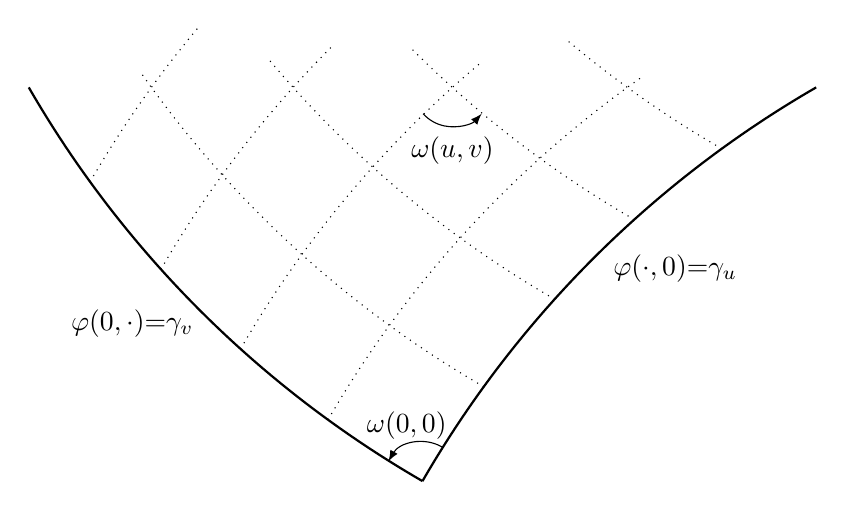
\begin{tikzpicture}[x=1cm,y=1cm]
    \pgfmathsetmacro{\cos}{cos(deg(60))}
    \pgfmathsetmacro{\sin}{sin(deg(60))}
    \draw[thick] (0,0) arc[start angle=150,delta angle=-30,radius=13.66] coordinate[pos=0.2] (u1) coordinate[pos=0.4] (u2) coordinate[pos=0.6] (u3) coordinate[pos=0.8] (u4);
    \coordinate (umid) at (2.3,2.7);
    \draw (umid) node[anchor=west]{$\varphi(\cdot,0){=}\gamma_u$};
    \draw[thick] (0,0) arc[start angle=-120,delta angle=-30,radius=13.66] coordinate[pos=0.2] (v1) coordinate[pos=0.4] (v2) coordinate[pos=0.6] (v3) coordinate[pos=0.8] (v4);
    \coordinate (vmid) at (-2.9,2.);
    \draw (vmid) node[anchor=east,inner sep=0pt]{$\varphi(0,\cdot){=}\gamma_v$};
   \draw[dotted] (u1) arc[start angle=-120,delta angle=-25,radius=13.66];
   \draw[dotted] (u2) arc[start angle=-120,delta angle=-20,radius=13.66];
   \draw[dotted] (u3) arc[start angle=-120,delta angle=-15,radius=13.66] coordinate[pos=0.8] (uv);
   \draw[dotted] (u4) arc[start angle=-120,delta angle=-10,radius=13.66];
   \draw[dotted] (v1) arc[start angle=150,delta angle=-25,radius=13.66];
   \draw[dotted] (v2) arc[start angle=150,delta angle=-20,radius=13.66];
   \draw[dotted] (v3) arc[start angle=150,delta angle=-15,radius=13.66];
   \draw[dotted] (v4) arc[start angle=150,delta angle=-10,radius=13.66];
   \draw[latex-] ($(uv)+(-42:0.5)$) arc[start angle=-42,delta angle=-96,radius=0.5];
   \draw ($(uv)+(-90:0.5)$) node[anchor=north]{$\omega(u,v)$};
 %   \draw[-latex] (0,0) -- (-30:1);
%    \draw ($(0,0)+(-45:0.4)$) node[anchor=north]{$\eta_1'(0)$};
 %   \draw[-latex] (0,0) -- (60:1);
%    \draw ($(0,0)+(130:0.9)$) node[anchor=west, inner sep=1pt]{$\eta_2'(0)$};
%    \draw[-latex] ($(0,0)+(-30:0.5)$) arc[start angle=-30, delta angle=90, radius=0.5];
%    \draw ($(0,0)+(15:0.5)$) node[anchor=west]{$\psi{=}\pi{-}\omega(0,0)$};
    \pgfmathsetmacro{\r}{0.5}
    \draw[-latex] (60:\r) arc[start angle=60, delta angle=90, radius=\r];
    \draw ($(90:.7)+(-.2,0)$) node{$\omega(0,0)$};
  \end{tikzpicture}
  \caption{Illustration of the coordinate curves of a Chebyshev net $\varphi$}\label{fig:hazz-primal-c4}
\end{figure}
We moreover remark that, since $\varphi$ is a Chebyshev net, it satisfies the following property:
\begin{subequations}\label{eq:courb-geod}
\begin{align}\label{eq:courb-geoda}
\kop_u(u,v) &= -\partial_u\omega(u,v), \\\label{eq:courb-geodb}
\kop_v(u,v) &= \partial_v\omega(u,v),
\end{align}
\end{subequations}
for all $(u,v)\in D$, where $\kop_u:D\to\R$ and $\kop_v:D\to\R$ are respectively the geodesic curvatures of the $u$-coordinate curves and of the $v$-coordinate curves of $\varphi$. We obtain by combining \eqref{eq:cond-bord-c3} and \eqref{eq:courb-geod} that the angle distribution $\omega$ satisfies the boundary conditions
\begin{subequations}\label{eq:cond-bord-angle}
\begin{align}
\omega(u, 0) &= \angle(\gamma_u'(0), \gamma_v'(0)) - \int_0^u\ko_u(s)\ds,\quad\forall u\in[0,L_u],\\
\omega(0,v) &= \angle(\gamma_u'(0), \gamma_v'(0)) + \int_0^v\ko_v(s)\ds,\quad\forall v\in[0,L_v].
\end{align}
\end{subequations}
We will first show that we can associate with any angle distribution $\omega:D\to\R/2\pi\Z$ satisfying \eqref{eq:cond-bord-angle} a unique mapping $\varphi:=\I(\gamma,\omega):D\to\surf$ satisfying \eqref{eq:cheb-def-c3b}, \eqref{eq:cond-bord-c3}, and \eqref{eq:courb-geodb}, and then we will show that this mapping also satisfies \eqref{eq:cheb-def-c3a} and \eqref{eq:courb-geoda} whenever $\omega$ satisfies the integrability condition \eqref{eq:cond-integr}. This section aims at proving the following result:
\begin{theorem}[Existence and uniqueness of Chebyshev nets]\label{thm2inexact}
Let $\surf$ be a smooth, open, complete, and simply connected surface. Let $\gamma_u:[0,L_u]\to\surf$, with $L_u\in\R_\ast^+$, and $\gamma_v:[0,L_v]\to\surf$, with $L_v\in\R_\ast^+$, be two curves with respective geodesic curvatures $\ko_u:[0,L_u]\to\R$ and $\ko_v:[0,L_v]\to\R$, and such that $\gamma_u(0) = \gamma_v(0)$. Suppose that $\angle(\gamma_1'(0),\gamma_2'(0))\in(0,\pi)$. Then, there exists a unique angle distribution $\omega:D\to\R/2\pi\Z$, with $D=[0,L_u]\Times[0,L_v]$, verifying the boundary conditions \eqref{eq:cond-bord-angle} and satisfying the Hazzidakis formula \eqref{eq:hazz-form}, with $\varphi:=\I(\gamma,\omega): D\to\surf$ the unique mapping satisfying \eqref{eq:cheb-def-c3b}, \eqref{eq:cond-bord-c3} and \eqref{eq:courb-geodb}.

Suppose moreover that we have $0<\omega(u,v)<\pi$, for all $(u,v)\in D$. Then, $\varphi$ is a Chebyshev net, i.e., it also satisfies \eqref{eq:cheb-def-c3a} and \eqref{eq:courb-geoda}, and the dependency of $\omega$ and $\varphi$ is continuous with respect to the boundary conditions $\gamma_u$ and $\gamma_v$.
\end{theorem}
In the previous statement, we have not defined precisely the regularity of the objects or the norms on the considered vector spaces. These are defined in Section \ref{sec:norms}, and a more accurate statement of Theorem \ref{thm2inexact} is given by Theorem \ref{thm2}. A direct consequence of Theorem \ref{thm2} is the following theorem:
\begin{theorem}[Existence of a unique solution to integrability condition]
  Let $\surf$ be a smooth, open, complete, and simply connected surface. Let $\gamma_u:[0,L_u]\to\surf$, with $L_u\in\R_\ast^+\cup\{\infty\}$, and $\gamma_v:[0,L_v]\to\surf$, with $L_v\in\R_\ast^+\cup\{\infty\}$, be two smooth curves with respective geodesic curvatures $\ko_u:[0,L_u]\to\R$ and $\ko_v:[0,L_v]\to\R$, and such that $\gamma_u(0) = \gamma_v(0)$. Suppose that $\angle(\gamma_u'(0),\gamma_v'(0))\in(0,\pi)$. Then, there exists a unique angle distribution $\omega:D\to\R/2\pi\Z$, with $D=[0,L_u]\Times [0,L_v]$, verifying the boundary conditions \eqref{eq:cond-bord-angle} and satisfying the Hazzidakis formula \eqref{eq:hazz-form}, with $\varphi:=\I(\gamma,\omega): D\to\surf$ the unique mapping satisfying \eqref{eq:cheb-def-c3b}, \eqref{eq:cond-bord-c3} and \eqref{eq:courb-geodb}.

  Suppose moreover that there exists $\tilde D=[0,\tilde L_u]\Times[0,\tilde L_v]$, with $\tilde L_u\in(0,L_u]$ and $\tilde L_v\in(0,L_v]$, such that $0<\omega(u,v)<\pi$, for all $(u,v)\in \tilde D$. Then, the mapping $\varphi\big|_{\tilde D}$ is a Chebyshev nets, that is, it satisfies \eqref{eq:cheb-def-c3} for all $(u,v)\in \tilde D$.
\end{theorem}

In order to prove Theorem \ref{thm2}, we proceed along the following plan. In Section \ref{subsec:constr-param}, given the two curves $\gamma_u$ and $\gamma_v$ on $\surf$ and the angle distribution $\omega:D\to\R/2\pi\Z$ between the coordinate curves, we first construct the candidate Chebyshev net $\varphi=\I(\gamma,\omega):D\to\surf$. We then show that whenever $\varphi$ satisfies the integrability condition \eqref{eq:cond-integr}, this mapping also satisfies \eqref{eq:cheb-def-c3} under suitable regularity conditions.  In Section \ref{subsec:exist-pt-fixe}, we view the Hazzidakis formula \eqref{eq:hazz-form}, with $\varphi:=\I(\gamma,\omega)$, as a fixed-point problem on $\omega$. We show existence and uniqueness of the solution to this fixed-point equation for the curves $\gamma_u$ and $\gamma_v\big|_{[0,L_0]}:[0,L_0]\to\surf$, where $L_0\in(0,L_v]$ is a constant depending on the $C^0$-norm of the geodesic curvatures of $\gamma_u$ and $\gamma_v$. This result is called ``local existence'' in what follows. We finally extend this result to the curves $\gamma_u$ and $\gamma_v$ of arbitrary length, in the spirit of the Cauchy--Lipschitz theorem.

\subsection{Functional spaces and statement of the main result}\label{sec:norms}

We now turn to the regularity required on the curves $\gamma_u$ and $\gamma_v$ and on the angle distribution $\omega$. In what follows, we define the spaces in which the curves, parametrizations and angles are constructed.  %When no confusion is possible, the mention of $L$, $L_u$ and $L_v$ will be dropped in the following notations for the sake of brevity.
Recall that
\begin{equation*}
  D=[0,L_u]\Times[0,L_v],\quad\text{with } L_u,L_v\in\R_\ast^+.
\end{equation*}
Let $k\in\EN$ and $L\in(0,L_v]$. We consider the space $C^{k+2}([0,L],\surf)$ of curves $\gamma$ with general parametrizations on $\surf$ and such that the geodesic curvature of $\gamma$ has $C^{k}$-regularity. % The space $W^{k+2,p}$, endowed with the norm
% \begin{equation}\label{normphi}
%   \|\gamma\|_{W^{k+2,p}} = |\gamma(0)|+|\gamma'(0)| + \|\gamma''\|_{W^{k,p}([0,L])},
% \end{equation}
% is a Banach space.
We define $\Gamma^{k+2}([0,L])$ to be the closed subset of $C^{k+2}([0,L],\surf)$ formed by arc-length parametrized curves:
\begin{equation*}  
  \Gamma^{k+2}([0,L]) = \Big\{\gamma \in C^{k+2}([0,L], \surf) \text{ s.t. } \forall s\in[0,L],~ |\gamma'(s)|_{g(\gamma(s))} = 1\Big\},
\end{equation*}
equipped with the norm $\|\cdot\|_{C^{k+2}([0,L])}$. Note that the norms involved in the Sobolev spaces are the Euclidean norms. Let $r\in\EN$. We define the space $\Theta^{r,k}(D)$ of angle distributions on $D$:
\begin{equation*}
  \Theta^{r,k}(D) = C^r\big([0,L_u],C^k([0,L_v], \R/2\pi\Z)\big),
\end{equation*}
equipped with the norm 
\begin{equation*}
  \|\omega\|_{\Theta^{r,k}(D)} = \|\omega\|_{C^r([0,L_u],C^k([0,L_v]))}.
\end{equation*}
 In the case where $k=r$, the notation of $\Theta^{k,k}(D)$ is simplified to $\Theta^k(D)$. We denote $\Phi^{r,k+2}(D)$ the closed subset of the Banach space $C^r([0,L_u],C^{k+2}([0,L_v],\surf))$ formed by arc-length parametrized curves with $C^{k+2}$-regularity depending on a parameter of regularity $C^r$:
\begin{equation*}  
  \Phi^{r,k+2}(D) := C^r\big([0,L_u], \Gamma^{k+2}([0,L_v])\big)\subset C^r\big([0,L_u],C^{k+2}([0,L_v],\surf)\big).
\end{equation*}
This space is equipped with the norm 
\begin{equation*}
  \|\varphi\|_{\Phi^{r,k+2}(D)} = \|\varphi\|_{C^r([0,L_u],\Gamma^{k+2}([0,L_v]))}.
\end{equation*}
 Note that we do not require the regularity on the first variable to be the same as the regularity on the second variable. This will be made visible in the construction of the candidate Chebyshev net $\varphi$: the first coordinate denotes the initial conditions of an ordinary differential equation in the second coordinate, which does not entail the same regularity.


Let $\gamma=(\gamma_u,\gamma_v)\in\Gamma^{r+2}([0,L_u])\Times \Gamma^{k+2}([0,L_v])$ be two curves with respective geodesic curvatures $\ko_u:[0,L_u]\to\R$ and $\ko_v:[0,L_v]\to\R$, and such that $\gamma_u(0)=\gamma_v(0)$. We define the affine subspace composed of the angle distributions satisfying the boundary conditions \eqref{eq:cond-bord-angle}:
\begin{equation*}  
    \Theta_{\gamma}^{r,k}(D) =
    \left\{ 
      % \begin{array}{c|c} 
      \omega \in \Theta^{r,k}(D),
    % \begin{array}{l}
  %     \displaystyle\omega(u, 0) = \angle(\gamma_u'(0), \gamma_v'(0)) - \int_0^u\ko_u(s)\ds,\\
  %     \displaystyle\omega(0,v) = \angle(\gamma_u'(0), \gamma_v'(0)) + \int_0^v\ko_v(s)\ds
  %   \end{array}\\
  % \end{array}
\text{ s.t. $\omega$ satisfies \eqref{eq:cond-bord-angle}}\right\}.
\end{equation*}
The subspace $\Theta^{r,k}_{\gamma}$ is a closed subset of the Banach space $\Theta^{r,k}$. Again, in the case where $r=k$, we set $\Theta_{\gamma}^k=\Theta_{\gamma}^{k,k}$.

We can now restate Theorem \ref{thm2inexact} with the correct regularity.
\begin{theorem}[Existence and uniqueness of Chebyshev nets]\label{thm2}
Let $\surf$ be a smooth, open, complete, and simply connected surface and let $k\in\EN$. Let $\gamma=(\gamma_u,\gamma_v)\in\Gamma^{k+2}([0,L_u])\Times\Gamma^{k+2}([0,L_v])$, with $L_u,L_v\in\R_\ast^+$, be two curves with respective geodesic curvatures $\ko_u\in C^k([0,L_u])$ and $\ko_v\in C^k([0,L_v])$, and such that $\gamma_u(0) = \gamma_v(0)$. Suppose that $\angle(\gamma_1'(0),\gamma_2'(0))\in(0,\pi)$. Then, there exists a unique angle distribution $\omega:=\J(\gamma) \in \Theta^{k+1}_{\gamma}(D)$, with $D=[0,L_u]\Times[0,L_v]$, verifying the boundary conditions \eqref{eq:cond-bord-angle} and satisfying the Hazzidakis formula \eqref{eq:hazz-form}, with $\varphi:=\I(\gamma,\omega)\in\Phi^{k+2}(D)$ the unique mapping satisfying \eqref{eq:cheb-def-c3b}, \eqref{eq:cond-bord-c3} and \eqref{eq:courb-geodb}. 

Suppose moreover that we have $0<\omega(u,v)<\pi$, for all $(u,v)\in D$. Then, $\varphi$ is a Chebyshev net, i.e., it also satisfies \eqref{eq:cheb-def-c3a} and \eqref{eq:courb-geoda}, and the mappings
\begin{equation*}
\begin{array}{cccc}
\J:&\Gamma^{k+2}([0,L_u])\Times\Gamma^{k+2}([0,L_v])&\to&\Theta^{k+1}(D),\\
  \I:&\Gamma^{k+2}([0,L_u])\Times\Gamma^{k+2}([0,L_v])\Times\Theta^{k+1}(D)&\to&\Phi^{k+2}(D)
\end{array}
\end{equation*}
are continuous.
\end{theorem}

\section{Construction of a Chebyshev net from its angle distribution}\label{subsec:constr-param}
We now prove that a Chebyshev net can be constructed uniquely from its angle distribution. We start by showing in Subsection \ref{subsec:construction} that the construction of curves from their geodesic curvature, initial point and initial tangent vector is a well-posed problem. We then define, following \cite{Ghys09}, the mapping $\I(\gamma,\omega)$ which, for given boundary curves $\gamma_u$ and $\gamma_v$, associates with any angle distribution $\omega$ satisfying the boundary conditions \eqref{eq:cond-bord-angle} the candidate Chebyshev net $\varphi$, with angle distribution $\omega$, satisfying the boundary conditions \eqref{eq:cond-bord-c3} (Subsection \ref{subsubsec:constr-param}). The parametrization $\varphi$ is constructed in such a way that the $v$-coordinate curves are arc-length parametrized curves with geodesic curvatures satisfying \eqref{eq:courb-geodb}. We moreover show the continuity of the mapping $\I$ with respect to the angle distribution and to the delimiting curves $\gamma_u$ and $\gamma_v$. In Subsection \ref{sec:reg-candidate}, we show that the candidate Chebyshev net $\varphi$ has improved regularity in the $u$-coordinate whenever $\omega$ satisfies the integrability condition \eqref{eq:cond-integr}. Finally, in Subsection \ref{sec:reg-cheb}, we prove that $\varphi$ is indeed a Chebyshev net if $\omega$ satisfies the integrability condition and has a sufficient regularity.

\subsection{Construction of curves from their geodesic curvature}\label{subsec:construction}
\begin{proposition}[Construction of curves from their geodesic curvature]\label{prop:constr-courbe}
 Let $\surf$ be a smooth, open, complete, and simply connected surface. Let $\Lmax\in\R^+_\ast$, $L\in(0,\Lmax)$ and $k,r\in\EN$. Let $x\in \surf$, let $V\in T_x\surf$ be a unit vector, i.e., a vector such that $|V|_g=1$, and let $\ko\in C^k([0,L],\R)$. Then, there exists a unique (arc-length parametrized) curve $\sigma(x,V,\ko):=\sigma\in \Gamma^{k+2}([0,L])$ such that $\sigma(0) = x$, $\sigma'(0) = V$, and with geodesic curvature $\ko$.

  Moreover, let $L_1,L_2\in(0,\Lmax)$, let $x_1,x_2\in C^r([0,L_1],\surf)$ be initial position distributions and let $V_1,V_2\in C^r([0,L_1],T\surf)$, with $|V_1|_g=|V_2|_g=1$, be initial derivatives distribution. Let $D_{1,2}=[0,L_1]\Times[0,L_2]$ and let $\ko_1, \ko_2 \in C^r([0,L_1],C^k([0,L_2],\R))$ be geodesic curvatures. We denote $\sigma_1,\sigma_2:[0,L_1]\to \Gamma^{k+2}([0,L_2])$ the two families of curves defined by $\sigma_m(\eta,\cdot):=\sigma(x_m(\eta),V_m(\eta),\ko_m(\eta,\cdot))$, for all $\eta\in[0,L_1]$ and $m\in\{1,2\}$. Then, we have
\begin{equation*}
\sigma_1,\sigma_2\in \Phi^{r,k+2}(D_{1,2})=C^r([0,L_1],\Gamma^{k+2}([0,L_2])),
\end{equation*}
and, for all $m\in\{1,2\}$, 
\begin{equation}\label{eq:borne-courbe}
\begin{split}
\|\sigma_m\|_{\Phi^{r,k+2}(D_{1,2})} \leq C,
\end{split}
\end{equation}
where the constant $C$ depends on $\Lmax$, $\|x_m\|_{C^r([0,L_1])}$, $\|V_m\|_{C^r([0,L_1])}$, and $\|\ko_m\|_{C^r([0,L_1],C^k([0,L_2]))}$.
Finally, we have%, for all $1\leq p\leq\infty$,
\begin{subequations}  \label{eq:estim-courbe}
\begin{align}\label{eq:estim-courbe1}
\begin{split}
  \|\sigma_1-\sigma_2\|_{\Phi^{0}(D_{1,2})} &\leq C\Big(L_2\|\ko_1-\ko_2\|_{C^0(D_{1,2})} \\
&  \quad+ \|x_1-x_2\|_{C^0([0,L_1])}+\|V_1-V_2\|_{C^0([0,L_1])}\Big),
\end{split}\text{ if $k=0$ and $r=0$,}\\\label{eq:estim-courbe2}
\begin{split}
  \|\sigma_1-\sigma_2\| _{\Phi^{r,k+2}(D_{1,2})}& \leq \tilde C\Big(\|\ko_1-\ko_2\|_{C^r([0,L_1],C^k([0,L_2]))} \\
  &\qquad+ \|x_1-x_2\|_{C^r([0,L_1])}+\|V_1-V_2\|_{C^r([0,L_1])}\Big),
\end{split}
\end{align}
\end{subequations}
where the constants $C$ and $\tilde C$ depend on $\Lmax$, $\|x_m\|_{C^r([0,L_1])}$, $\|V_m\|_{C^r([0,L_1])}$, and $\|\ko_m\|_{C^r([0,L_1],C^k([0,L_2]))}$, with $m\in\{1,2\}$.
\end{proposition}
We illustrate the family of curves $\sigma_1$ introduced in Proposition \ref{prop:constr-courbe} in Figure \ref{fig:construction}.
\begin{figure}[!htp]
  \centering
  \begin{tikzpicture}[x=1.8cm,y=1.8cm]
    \draw[red] (0,0) node[anchor=north east,inner sep=1pt]{$x_1(0)$};
    \draw[red] (0,0) node{$\times$};
    \draw[thick,red] (0,0) arc[start angle=110,delta angle=-40,radius=5] coordinate[pos=0.5] (v1) coordinate[pos=0.3] (v2);
    \draw[thick] (0,0) arc[start angle=200,delta angle=-40,radius=5] coordinate[pos=0.5] (v3);
    \draw (v3) node[anchor=east]{$\sigma_1(0,\cdot)$};
    \draw (v2) arc[start angle=180,delta angle=-40,radius=5] coordinate[pos=0.5] (v4)  coordinate[pos=0.7] (v5);
    \draw (v4) node[anchor=east]{$\sigma_1(\eta,\cdot)$};
    \draw[red] (v2) node[anchor=north]{$x_1(\eta)$};
    \draw[red] (v2) node{$\times$};
    \draw[-latex,red] (v2) -- ($(v2)+(90:.6)$) node[pos=0.4,anchor=south east]{$V_1(\eta)$};
    \draw[-latex,red] (0,0) -- ($(110:.6)$) node[pos=0.4,anchor= east]{$V_1(0)$};
    \draw (v5) node[anchor=east]{$\sigma_1(\eta,s)$};
    \draw (v5) node{$\times$};
   \end{tikzpicture}
  \caption{Illustration of the construction of the family of curves $\sigma_1$}\label{fig:construction}
\end{figure}
\begin{proof}
  To prove the claim, we proceed as follows. We first introduce in Step \ref{step:geod-eq} the geodesic curvature equation that permits to define uniquely a curve from its geodesic curvature. The existence and the uniqueness of the curve is proved in Step \ref{step:init-induc} using Cauchy--Lipschitz theorem. Then, in order to apply an induction argument, we prove \eqref{eq:borne-courbe} and \eqref{eq:estim-courbe} in the case $k=0$ and $r=0$ using Grönwall's inequality. The equation satisfied by the derivatives of the solution is presented in a generic form to facilitate the end of the proof in Step \ref{step:diff-eq}. Finally, we prove \eqref{eq:borne-courbe} and \eqref{eq:estim-courbe2} in Steps \ref{step:borne} and \ref{step:control} using induction arguments. Whenever there is no ambiguity, the domain of the variables will be omitted.
  \begin{proofpart}[Formulation of the geodesic curvature equation]\label{step:geod-eq}
  Let $(\sigma^1,\sigma^2)$, with $\sigma^1,\sigma^2:[0,L]\to\R$, be the coordinates of the candidate curve $\sigma:[0,L]\to\surf$ with geodesic curvature $\ko$. %The proof follows directly by application of Carathéodory's existence theorem \cite{Har64}, Grönwall's and Jensen's inequalities on
 We denote $\frac{D}{dt}$ the covariant derivative along the curve $\sigma$. The geodesic curvature equation for arc-length parametrized curves gives
\begin{equation}
\label{eq:geod-curv}
  \frac{D}{dt}\sigma' = \ko\sigma^{\prime\perp},
\end{equation}
which can be written, in coordinates,
\begin{equation}
\label{eq:pr-edo}
  \dot X = G(X) + \ko f(X),
\end{equation}
with $X(0)=(x^1,x^2,V^1,V^2)$. Here, we have denoted
\small
\begin{equation*}
  X = 
\left(
\begin{array}{c}
\sigma^1\\\sigma^2\\\sigma^{\prime 1}\\\sigma^{\prime 2} 
\end{array}\right), \quad
f(X) = \left( 
  \begin{array}{c}
    0\\0\\N^1\\N^2
    \end{array} \right), \quad
G(X) = \left(
  \begin{array}{c}
    X^3\\ X^4\\\displaystyle -\sum_{1\leq i,j\leq 2}\Gamma_{i,j}^1(X^1,X^2)X^{2+i}X^{2+j}\\ 
\displaystyle-\sum_{1\leq i,j\leq 2}\Gamma_{i,j}^2(X^1,X^2)X^{2+i}X^{2+j}
  \end{array}\right),
\end{equation*}
\normalsize
$\Gamma_{ij}^{k}$ being the smooth Christoffel symbols, $G$ the smooth geodesic function and $N$ the normal vector defined by
\begin{equation*}
N = \left(\begin{array}{c}
N^1\\N^2
\end{array}\right)
= \sqrt{\det g(X^1,X^2)}g^{-1}(X^1,X^2)
  \left(\begin{array}{c}
      -X^4\\X^3
      \end{array}\right).
\end{equation*}
%We prove the assertions of the proposition by induction on $k\geq0$ and $r\geq0$.
\end{proofpart}

\begin{proofpart}[Proof for $k=0$ and $r=0$]\label{step:init-induc}
%\paragraph*{Proof for $k=0$ and $r=0$.}
  As $G+\ko f$ is continuous and locally Lipschitz continuous with respect to $X$, owing to Cauchy--Lipschitz theorem, there exists a local solution to \eqref{eq:pr-edo}. Moreover, since $\sigma$ is by construction arc-length parametrized, we have $|\sigma'|_g=1$ and we infer from \eqref{eq:equiv} that $|\sigma'|\leq\Csurf$. Hence, the image of $X$ is included in a ball $\B$ whose radius depends only on $\Lmax$ and $\Csurf$. We deduce that the solution is defined on $[0,L]$. Moreover, $G$ and $f$ are Lipschitz continuous with respect to $X$ on $\B$. Hence, $G+\ko f$ is Lipschitz continuous with respect to $X$ on $\B$, so that the uniqueness of the solution follows. Moreover, we infer from \eqref{eq:pr-edo} that $\sigma\in\Gamma^{2}([0,L])$.

  Let $m\in\{1,2\}$ and let $X_m = (\sigma_m^1, \sigma_m^2, \sigma_m^{\prime 1}, \sigma_m^{\prime 2})^t:D_{1,2}\to\R^4$ be such that $X_m(\eta,\cdot)$ is the unique solution to \eqref{eq:pr-edo} with $\ko=\ko_m(\eta,\cdot)$, for all $\eta\in[0,L_1]$. First, owing to \cite[Chap. V, Th. 2.1]{Har64}, we have $X_m\in C^0([0,L_1], C^1([0,L_2]))$, so that $\sigma_m\in \Phi^{0,2}(D_{1,2})$. Then, since $|\sigma'|\leq\Csurf$, we infer that $\|\sigma_m\|_{\Phi^{0,2}(D_{1,2})}\leq C$, where the constant $C$ depends on $\|\sigma_m(\cdot,0)\|_{C^0([0,L_1])}$ and $\|X_m'\|_{C^0(D_{1,2})}$. Moreover, due to $|f(X_m)|_g = |\sigma_m'|_g=1$, we have
  \begin{equation}\label{eq:pr-bound-f}
    |f(X_m)|\leq \Csurf.
  \end{equation}
Furthermore, since $X_m(\{\eta\}\times[0,L_2])\subset \B$, we infer that $G(X_m)$ is bounded and that this bound only depends on $\B$, so that it only depends on $X_m(\eta,0)$, $\Lmax$ and $\Csurf$, for all $\eta\in[0,L_1]$. We conclude that
\begin{equation*}
  \|\sigma_m\|_{\Phi^{0,2}(D_{1,2})}\leq C,
\end{equation*}
where the constant $C$ depends on $\|x_m\|_{C^0([0,L_1])}$ and $\|\ko_m\|_{C^0(D_{1,2})}$, and \eqref{eq:borne-courbe} holds with $k=r=0$.
Then, since the restrition of $G$ and $f$ to $\B$ are Lipschitz continuous in the variable $X$ with coefficients denoted respectively $C_G$ and $C_f$, we have  
\begin{equation*}
  |\dot X_1 - \dot X_2| \leq (C_G+|\ko_1| C_f)|X_2-X_1|+|\ko_2-\ko_1| \ \|f(X_2)\|_{C^0(D_{1,2}))}.
\end{equation*} 
Therefore, using Grönwall's inequality and \eqref{eq:pr-bound-f}, we infer that
\small
\begin{equation}
 \label{eq:reg-equ-geod}
 |X_1(t)-X_2(t)| \leq
  \exp\Big[t\big(C_G+C_f \|\ko_1\|_{C^0(D_{1,2})}\big)\Big]\left(|X_2(0) - X_1(0)| + \Csurf\int_0^t \left|\ko_2 - \ko_1\right| \right),
\end{equation}
\normalsize
for all $t\in[0,L]$. We deduce that \eqref{eq:estim-courbe1} and \eqref{eq:estim-courbe2} are satisfied for $k=r=0$. % and $p=\infty$. 
% Now, suppose that $1\leq p<\infty$. By Jensen's inequality and \eqref{eq:reg-equ-geod}, we have 
% \begin{align*}
%   |X_1(t)-X_2(t)|^p &\lesssim |X_2(0) - X_1(0)|^p + \Big(\int_0^t \left|\ko_2 - \ko_1\right|\Big)^p \\
%   &\lesssim |X_2(0) - X_1(0)|^p + t^{p-1}\int_0^t \left|\ko_2 - \ko_1\right|^p.
% \end{align*}
% We easily conclude that \eqref{eq:estim-courbe1} and \eqref{eq:estim-courbe2} are satisfied with $k=0$, $r=0$ and $p<\infty$.
\end{proofpart}

\begin{proofpart}[Differential equation on the derivatives of $X$]\label{step:diff-eq}
%\paragraph*{Differential equation on the derivatives of $X$.}
Let $m\in\{1,2\}$. Owing to \cite[Chap. V, Th. 4.1]{Har64}, we have that $\sigma\in \Gamma^{k+2}([0,L])$ and $\sigma_m\in \Phi^{r,k+2}(D_{1,2})$.
We use the following notation: for $I=(i_1,i_2)\in \EN^2$, we set $\DI f(\eta,t) = \partial_\eta^{i_1}\partial^{i_2}_t f(\eta,t)$. 
We denote $(\H_{r,k})$, with $r,k\in\EN^\ast$, the following induction hypothesis:

\textit{for all $I=(i_1,i_2)\in\{0,...,r\}\Times\{0,...,k\}$ such that $I\neq (0,0)$, we have
\begin{equation}\label{eq:eq-der-courbe}
\begin{split}
\partial_t \DI X_m = &~~(\nabla G(X_m)+\ko_m\nabla f(X_m))\DI X_m \\
&+ \sum_{0\leq\alpha\leq i_1}\sum_{0\leq\beta\leq i_2}F^I_{\alpha,\beta}\left[(\partial^{(p,q)}X_m)_{0\leq p+\alpha \leq i_1,~0\leq q+\beta\leq i_2,~p+q<i_1+i_2}\right] \partial^{(\alpha,\beta)}\ko_m,
\end{split}
\end{equation}
where $F^I_{\alpha,\beta}:\R^{4n_0}\to \R^4$, with
\begin{equation*}
 n_0=\left\{\begin{split}
 &(i_1-\alpha+1)(i_2-\beta+1), &\quad\text{if } \alpha+\beta\neq0,\\
  &(i_1+1)(i_2+1)-1, &\quad\text{otherwise},
\end{split}\right.
\end{equation*}
are $C^\infty$ functions, for all $(\alpha,\beta)\in\{0,...,i_1\}\Times\{0,...,i_2\}$. %Moreover, $F^I_{\alpha,\beta}$ is polynomial in $\partial^{(p,q)}X_m$, with $(p,q)\in\{0,...,i_1-\alpha\}\Times\{0,...,i_2-\beta\}$ such that $(p,q)\neq(0,0)$, for all $(\alpha,\beta)\in\{0,...,i_1\}\Times\{0,...,i_2\}$.
}

We denote $\partial_1$ and $\partial_2$ the derivatives with respect to $\eta$ and $t$ respectively. We first obtain from \eqref{eq:pr-edo} that,
 for all $m\in\{1,2\}$ and $i\in\{1,2\}$, 
\begin{equation*}
 \partial_t \partial_i X_m = \nabla G(X_m)\partial_i X_m 
 + \partial_i \ko_m f(X_m) + \ko_m\nabla f(X_m) \partial_i X_m.
\end{equation*}
Hence, \eqref{eq:eq-der-courbe} is satisfied for $I=(0,1)$ and $I=(1,0)$, so that $(\H_{1,1})$ holds. We now suppose that $(\H_{r,k})$ holds for $r,k\in\EN^\ast$. Then, for $I=(i_1,i_2)$ with $i_1=r$ and $i_2=k$, we have 
\begin{align*}
\partial_t\partial_i\DI X_m &= (\nabla G(X_m)+\ko_m\nabla f(X_m))\partial_i\DI X_m + \partial_i\big[\nabla G(X_m)+\ko_m\nabla f(X_m)\big]\DI X_m \\
&\quad+ \sum_{0\leq\alpha\leq i_1}\sum_{0\leq\beta\leq i_2}\bigg[\partial_i \left(F^I_{\alpha,\beta}\left[(\partial^{(p,q)}X_m)_{0\leq p+\alpha \leq i_1,~0\leq q+\beta\leq i_2, ~p+q<i_1+i_2}\right]\right) \partial^{(\alpha,\beta)}\ko_m \\
  &\qquad\qquad\qquad\qquad\quad+ F^I_{\alpha,\beta} \partial_i\partial^{(\alpha,\beta)}\ko_m\bigg].
\end{align*}
The first term is in the form of the first term on the right-hand side of \eqref{eq:eq-der-courbe} and the last two terms can be put in the form of the second term on the right-hand side of \eqref{eq:eq-der-courbe}. Equation \eqref{eq:eq-der-courbe} is then satisfied for $I=(r+1,k)$ and $I=(r,k+1)$, so that $(\H_{r+1,k})$ and $(\H_{r,k+1})$ hold. The claim follows.
\end{proofpart}

\begin{proofpart}[Proof of \eqref{eq:borne-courbe}]\label{step:borne}
%\paragraph*{Proof of \eqref{eq:borne-courbe}.}
Let $m\in\{1,2\}$. First note that we have by definition
\begin{align*}
\|\sigma_m\|_{\Phi^{r,k+2}(D_{1,2})} &\leq  \sum_{i_1=0}^{r}\sum_{i_2=0}^{k+1}\|\partial_{\eta}^{i_1}\partial_{t}^{i_2}X_m\|_{C^0(D_{1,2})}.
\end{align*}
Then, to obtain \eqref{eq:borne-courbe}, we only need to prove that
\begin{equation}\label{eq:pr-borne-courbe}
  \|\DI X_m\|_{C^0(D_{1,2})} \leq C,
\end{equation}
where the constant $C$ depends on $\Lmax$, $\|x_m\|_{C^{i_1}([0,L_1])}$, $\|V_m\|_{C^{i_1}([0,L_1])}$, and $\|\ko_m\|_{C^{i_1}([0,L_1],C^{i_2}([0,L_2]))}$,
for all $I=(i_1,i_2)\in\{0,...,r\}\Times\{0,...,k{+}1\}$. We prove \eqref{eq:pr-borne-courbe} by induction on $I\in\{0,...,r\}\Times\{0,...,k+1\}$. Hence, we first consider the case $i_2=0$, in which case we have, using \eqref{eq:eq-der-courbe} and Grönwall's inequality,
\begin{equation*}
\begin{split}
|\partial_\eta^{i_1}X_m(t)|\leq&\exp\big[\|\nabla G(X_m) +\ko_{\sigma_m}\nabla f(X_m)\|_{C^0(D_{1,2})}t\big]\\
&\Times\Big(|\partial_\eta^{i_1} X_m(0)| + \sum_{\alpha=0}^{i_1}\int_0^t\left|F_{\alpha,0}^{(i_1,0)}\left[X_m,..,\partial_\eta^{i_1-1}X_m\right]\partial^{(\alpha,0)}\ko_{\sigma_m}\right|\Big),
\end{split}
\end{equation*}
for all $i_1\in\{1,...,r\}$. Moreover, from Step \ref{step:init-induc}, we have that \eqref{eq:pr-borne-courbe} holds in the case where $I=(0,0)$. Then, since the functions $F^{(i_1,0)}_{\alpha,0}$ have $C^\infty$-regularity with respect to $(X_m,...,\partial^{i_1-1}_\eta X_m)$, for all $\alpha\in\{0,...,i_1\}$ and $i_1\in\{1,...r\}$, an induction argument on $i_1\in\{0,...,r\}$ permits to prove that \eqref{eq:pr-borne-courbe} holds for all $I\in\{0,...,r\}\Times\{0\}$.
 
%Now, let $I\in\{0,...,r\}\Times\{1,...,k+1\}$. 
Now, noting that $\partial_t\DI X_m = \partial_{\eta}^{i_1}\partial_{t}^{i_2+1}X_m$, we infer from \eqref{eq:eq-der-courbe} that
\small
\begin{multline*}
\|\partial_t\DI X_m\|_{C^0(D_{1,2})} \leq ~~\|\nabla G(X_m) + \ko\nabla f(X_m)\|_{C^0(D_{1,2})}\|\DI X_m\|_{C^0(D_{1,2})} \\
+ \sum_{0\leq\alpha\leq i_1}\sum_{0\leq\beta\leq i_2}\Big\|F^I_{\alpha,\beta}\left[(\partial^{(p,q)}X_m)_{0\leq p+\alpha \leq i_1,~0\leq q+\beta\leq i_2,~p+q<i_1+i_2}\right]\Big\|_{C^0(D_{1,2})}\|\partial^{(\alpha,\beta)}\ko_m\|_{C^0(D_{1,2})},
\end{multline*}
\normalsize
for all $I=(i_1,i_2)\in\{0,...,r\}\Times\{0,...,k\}$ such that $I\neq(0,0)$. Finally, since \eqref{eq:pr-borne-courbe} holds for all $I=(i_1,0)\in\{0,...,r\}\Times\{0\}$ and for $I=(0,1)$ by step \ref{step:init-induc}, and since all the functions $F^I_{\alpha,\beta}$ have $C^\infty$-regularity, the induction argument on $I$ to prove that \eqref{eq:pr-borne-courbe} holds for all $I\in\{0,...,r\}\Times\{0,...,k{+}1\}$ is straightforward. We conclude that \eqref{eq:borne-courbe} holds.
%The result for $i_2=0$ is a simple adaptation of \cite[Chap. V, Th. 4.1]{Har64}.
\end{proofpart}

\begin{proofpart}[Proof of \eqref{eq:estim-courbe2}]\label{step:control}
  %\paragraph*{Proof of \eqref{eq:estim-courbe}.}
  Let $I=(i_1,i_2)\in\{0,...,r\}\Times\{0,...,k\}$ be such that $I\neq(0,0)$ and let $m\in\{1,2\}$. Owing to \eqref{eq:borne-courbe}, $\partial^{\tilde I} X_m$ is bounded by a constant depending only on $\|\ko_m\|_{C^r([0,L_1],C^k([0,L_2])}$, $\|x_m\|_{C^r([0,L_1])}$, and $\|V_m\|_{C^r([0,L_1])}$, for all $\tilde I\in\{0,...,r\}\Times\{0,...,k\}$. Hence, the smooth functions $F_{\alpha,\beta}^I$ are Lipschitz continuous on the compact set defined by the image of the derivatives of $X_m$, for all $(\alpha,\beta)\in\{0,...,i_1\}\Times\{0,...,i_2\}$. We denote $C_{F_{\alpha,\beta}^I}$ their respective Lipschitz coefficients in this compact set and we set $W_m=\DI X_m$. Using \eqref{eq:eq-der-courbe}, we easily obtain that
\small
\begin{equation*}%\label{eq:pr-estim-der}
  \begin{split}
|\partial_t W_2& - \partial_t W_1| \leq \big(\|\nabla G(X_1)\|_{C^0}+|\ko_1|\|\nabla f(X_1)\|_{C^0}\big)|W_2-W_1| \\
&\qquad\qquad~~+ \Big(\big|\ko_1\nabla f(X_1)-\ko_2\nabla f(X_2)\big|+\big|\nabla G(X_1)-\nabla G(X_2)\big|\Big)\|W_2\|_{C^0}\\
&\qquad\qquad~~+ \sum_{\alpha=0}^{i_1}\sum_{\beta=0}^{i_2} C_{F^I_{\alpha,\beta}}\sum_{\substack{p\in\{0,...,i_1\},~q\in\{0,...,i_2\}\\p+q<i_1+i_2}}\big|\partial^{(p,q)}X_2-\partial^{(p,q)} X_1\big| \|\partial^{(\alpha,\beta)}\ko_1\|_{C^0}\\
&+\sum_{\alpha=0}^{i_1}\sum_{\beta=0}^{i_2} \left\|F^I_{\alpha,\beta}\left[(\partial^{(p,q)}X_2)_{0\leq p+\alpha \leq i_1,~0\leq q+\beta\leq i_2,~p+q<i_1+i_2}\right]\right\|_{C^0}|\partial^{(\alpha,\beta)}\ko_1-\partial^{(\alpha,\beta)}\ko_2|,
\end{split}
\end{equation*}
\normalsize
where $C^0$ refers to the norm $C^0(D_{1,2})$. Using Grönwall's inequality, we infer that
\small
\begin{align*}
  &|W_1-W_2|(\eta,t)\leq \exp\big[\|\nabla G(X_1) +\ko_1\nabla f(X_1)\|_{C^0}t\big]\times\\
  &~~\bigg( |W_1-W_2|(\eta,0) + \|W_2\|_{C^0}\max_{i\in\{1,2\}}\max\big(\|\ko_i\|_{C^0},\|\nabla f(X_i)\|_{C^0},1\big) \int_0^t\big[|\ko_2-\ko_1|{+}\big(C_{\nabla f}{+}C_{\nabla G}\big)|X_2-X_1|\big]\\
  &\qquad\qquad\qquad~~+\sum_{\alpha=0}^{i_1}\sum_{\beta=0}^{i_2}C_{F^I_{\alpha,\beta}} 
\|\partial^{(\alpha,\beta)}\ko_1\|_{C^0}\sum_{\substack{p\in\{0,...,i_1\},~q\in\{0,...,i_2\}\\p+q<i_1+i_2}}\int_0^t|\partial^{(p,q)}X_2-\partial^{(p,q)}X_1| \\
&\qquad\qquad\qquad~~+ \sum_{\alpha=0}^{i_1}\sum_{\beta=0}^{i_2}
\left\|F^I_{\alpha,\beta}\left[(\partial^{(p,q)}X_2)_{0\leq p+\alpha \leq i_1,~0\leq q+\beta\leq i_2,~p+q<i_1+i_2}\right]\right\|_{C^0}\int_0^t\big|\partial^{(\alpha,\beta)}\ko_1-\partial^{(\alpha,\beta)}\ko_2\big|\bigg),
\end{align*}
\normalsize
where $C^0$ refers to the norm $C^0(D_{1,2})$, and $C_{\nabla f}$ and $C_{\nabla G}$ are the Lipschitz constants of $\nabla f$ and $\nabla G$, respectively. Then, %such as in Step \ref{step:init-induc}, 
we obtain using \eqref{eq:borne-courbe} that % and Jensen's inequality whenever $p<\infty$ that
\begin{align*}
  \|\sigma_1-\sigma_2\|_{\Phi^{i_1,i_2+1}(D_{1,2})} \leq C\Big(&\|\ko_1-\ko_2\|_{C^{i_1}([0,L_1],C^{i_2}([0,L_2]))} + \|x_1-x_2\|_{C^{i_1}([0,L_1])}\\
&  + \|V_1-V_2\|_{C^{i_1}([0,L_1])} + \Sigma_1+\Sigma_2\Big),
\end{align*}
where the constant $C$ depends on $\Lmax$, $\|x_l\|_{C^{i_1}([0,L_1])}$, $\|V_l\|_{C^{i_1}([0,L_1])}$, and $\|\ko_l\|_{C^{i_1}([0,L_1],C^{i_2}([0,L_2]))}$, with $l\in\{1,2\}$, and
\begin{equation*}
  \Sigma_1=\begin{cases}
    \|\sigma_1-\sigma_2\|_{\Phi^{i_1-1,i_2+1}(D_{1,2})},&\text{if $i_1>0$,}\\
    0, &\text{otherwise,}
\end{cases}\quad\Sigma_2=\begin{cases}
    \|\sigma_1-\sigma_2\|_{\Phi^{i_1,i_2}(D_{1,2})},&\text{if $i_2>0,$}\\
    0, &\text{otherwise}.
\end{cases}
\end{equation*}
Hence, using \eqref{eq:eq-der-courbe}, we obtain in the same manner that
\begin{align*}
  \|\sigma_1-\sigma_2\|_{\Phi^{i_1,i_2+2}(D_{1,2})} \leq C\Big(&\|\ko_1-\ko_2\|_{C^{i_1}([0,L_1],C^{i_2}([0,L_2]))} + \|x_1-x_2\|_{C^{i_1}([0,L_1])}\\
&  + \|V_1-V_2\|_{C^{i_1}([0,L_1])} + \Sigma_1+\Sigma_2\Big),
\end{align*}
where the constant $C$ depends on $\Lmax$, $\|x_l\|_{C^r([0,L_1])}$, $\|V_l\|_{C^r([0,L_1])}$, and $\|\ko_l\|_{C^r([0,L_1],C^k([0,L_2]))}$, with $l\in\{1,2\}$.
We then obtain \eqref{eq:estim-courbe} by a straightforward induction argument on $I=(i_1,i_2)\in\{0,...,r\}\Times\{0,...,k\}$, recalling that the case $I=(0,0)$ was proved in Step \ref{step:init-induc}. This concludes the proof of the proposition.
\end{proofpart}
\end{proof}

\subsection{Construction of the parametrization}\label{subsubsec:constr-param}

Let $\RR_x(\theta)$ be the rotation of angle $\theta$ in the tangent plane $T_x\surf$ at $x\in \surf$ and let $D=[0,L_u]\times[0,L_v]$, with $L_u,L_v\in\R^+_\ast$. Let $r,k\in\EN$. Using the notation of Proposition \ref{prop:constr-courbe}, given an angle distribution $\omega\in\Theta^{r+1,k+1}_{\gamma}(D)$ satisfying the boundary conditions \eqref{eq:cond-bord-angle} given by the two curves $\gamma=(\gamma_u,\gamma_v)\in\Gamma^{r+2}([0,L_u])\Times \Gamma^{k+2}([0,L_v])$, we set 
\begin{equation}\label{eq:constr-cheb}
  x(\eta)=\gamma_u(\eta)\in\surf,\quad V(\eta) = \RR_{\gamma_u(\eta)}(\omega(\eta,0))\gamma_u'(\eta)\in T_{\gamma_u(\eta)}\surf,
\end{equation}
and $\ko(\eta,s) = \partial_v\omega(\eta,s)$, for all $(\eta,s)\in D$. Let $\varphi_\omega:D\to\surf$ be the family of curves such that the curve $\varphi_\omega(\eta,\cdot)\in\Gamma^{k+2}([0,L_v])$ has initial position $\varphi_\omega(\eta,0) = x(\eta)$, initial tangent vector $\partial_v\varphi_\omega(\eta,0) = V(\eta)$, and geodesic curvature $\ko(\eta,\cdot)$, for all $\eta\in[0,L_u]$ (see Figure \ref{fig:construction2}). Note that the mapping $\varphi_\omega$ also depends on the curves $\gamma=(\gamma_u,\gamma_v)$ but since these curves are kept fixed in what follows, we do not mention them explicitly. We denote
\begin{equation*}%  \label{eq:def-cheb}
  \begin{split}
    \I(\gamma,\cdot) : \Theta^{r+1,k+1}_\gamma(D) & \to \Phi^{r+1,k+2}(D), \\
     \omega & \mapsto \varphi_\omega,
\end{split}
\end{equation*}
the mapping that associates with each angle distribution $\omega$ with $\Theta^{r+1,k+1}$-regularity and satisfying the boundary conditions \eqref{eq:cond-bord-angle}, the mapping $\varphi_\omega : D \to \surf$.

\begin{figure}[!htp]
  \centering
  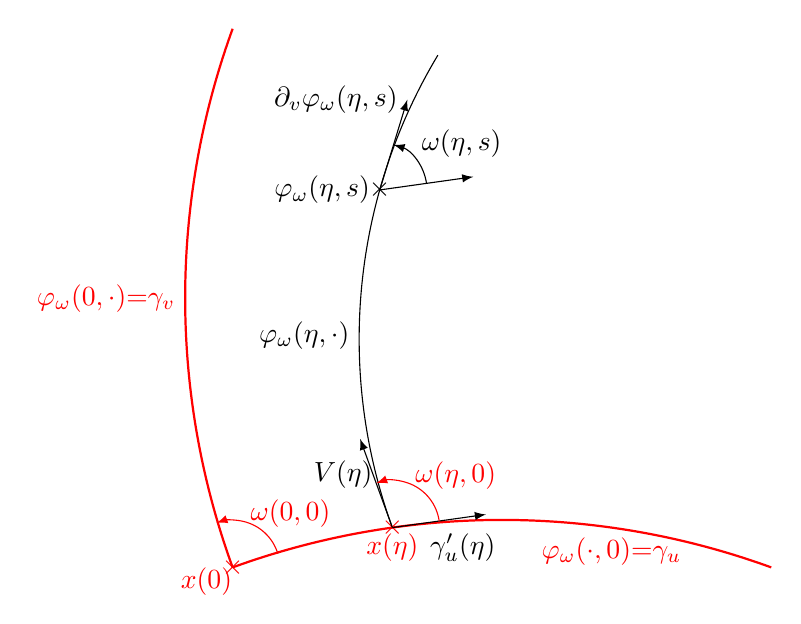
\begin{tikzpicture}[x=2cm,y=2cm]
    \draw[red] (0,0) node[anchor=north east,inner sep=0pt]{$x(0)$};
    \draw[red] (0,0) node{$\times$};
    \draw[thick,red] (0,0) arc[start angle=110,delta angle=-40,radius=5] coordinate[pos=0.7] (v1) coordinate[pos=0.3] (v2);
    \draw[red] (v1) node[anchor=north]{$\varphi_\omega(\cdot,0){=}\gamma_{u}$};
    \draw[thick,red] (0,0) arc[start angle=200,delta angle=-40,radius=5] coordinate[pos=0.5] (v3);
    \draw[red] (v3) node[anchor=east]{$\varphi_\omega(0,\cdot){=}\gamma_{v}$};
    \draw (v2) arc[start angle=200,delta angle=-51,radius=3.5] coordinate[pos=0.4] (v4)  coordinate[pos=0.7] (v5);
    \draw (v4) node[anchor=east]{$\varphi_\omega(\eta,\cdot)$};
    \draw[red] (v2) node[anchor=north,inner sep=2pt]{$x(\eta)$};
    \draw[red] (v2) node{$\times$};
    \draw[-latex] (v2) -- ($(v2)+(8:.6)$) node[anchor=north west,pos=.3]{$\gamma_u'(\eta)$};
    \draw[-latex] (v2) -- ($(v2)+(110:.6)$) node[anchor=east, inner sep=0pt,pos=.6]{$V(\eta)$};
    \draw[-latex,red] ($(v2)+(8:0.3)$) arc[start angle=8,delta angle=102,radius=0.3];
    \draw[red] ($(v2)+(65:0.2)$) node[anchor=south west]{$\omega(\eta,0)$};
    \draw[red] ($(75:0.2)$) node[anchor=south west]{$\omega(0,0)$};
    \draw (v5) node[anchor=east]{$\varphi_\omega(\eta,s)$};
    \draw (v5) node{$\times$};
    \draw[-latex] (v5) -- ($(v5)+(73:.6)$) node[anchor=east]{$\partial_v\varphi_\omega(\eta,s)$};
    \draw[-latex] (v5) -- ($(v5)+(8:.6)$);
    \draw[-latex] ($(v5)+(8:0.3)$) arc[start angle=8,delta angle=65,radius=0.3];
    \draw ($(v5)+(35:0.25)$) node[anchor=south west]{$\omega(\eta,s)$};
    \draw[-latex,red] ($(17:0.3)$) arc[start angle=17,delta angle=93,radius=0.3];
  \end{tikzpicture}
  \caption{Illustration of the construction of the parametrization $\varphi_\omega$}\label{fig:construction2}
\end{figure}

\begin{proposition}[Continuity of the construction]\label{prop:cont-I}
Let $\surf$ be a smooth, open, complete, and simply connected surface, let $k,r\in\EN$, and let $D=[0,L_u]\Times[0,L_v]$, with $L_u,L_v\in\R^+_\ast$. For all $\gamma=(\gamma_u,\gamma_v)\in\Gamma^{r+2}([0,L_u])\Times\Gamma^{k+2}([0,L_v])$, the mapping $\I(\gamma,\cdot)$ is well defined. Moreover, let \sloppy $\gamma_1,\gamma_2\in\Gamma^{r+2}([0,L_u])\Times\Gamma^{k+2}([0,L_v])$, with $\gamma_1=(\gamma_{u,1}, \gamma_{v,1})$ and $\gamma_2=(\gamma_{u,2}, \gamma_{v,2})$, be such that $\gamma_{u,1}(0)=\gamma_{u,2}(0) = \gamma_{v,1}(0)=\gamma_{v,2}(0)$ and such that $\gamma_{u,1}'(0)=\gamma_{u,2}'(0)$ and $\gamma_{v,1}'(0)=\gamma_{v,2}'(0)$. Consider the two angle distributions $\omega_m\in \Theta^{r+1,k+1}_{\gamma_m}(D)$, for $m\in\{1,2\}$. Then, we have
\begin{equation}\label{eq:contr-I}
  \|\I(\gamma_m,\omega_m)\|_{\Phi^{r+1,k+2}(D)} \leq C%\left(\|\gamma_{u,m}\|_{\Gamma^{r+1}([0,L_u])},\|\omega_m\|_{\Theta^{r+1,k+1}(D)}\right), \text { if } r>0,
\end{equation}
where the constant $C$ depends on $L_u$, $L_v$, $\|\gamma_{u,m}\|_{\Gamma^{s}([0,L_u])}$, and $\|\omega_m\|_{\Theta^{r+1,k+1}(D)}$, with $s=\max(r+1,2)$.
Moreover, for all $L\in(0,L_v]$, setting $D_L=[0,L_u]\Times[0,L]$, we have
\small
\begin{subequations}\label{eq:cont-I}
\begin{align}\label{eq:cont-I1}
\begin{split}
  \|\I(\gamma_1,\omega_1) - \I(\gamma_2,\omega_2)\|_{\Phi^{0}(D_L)} &\leq ~C\Big(L\|\omega_1 - \omega_2\|_{\Theta^{1}(D_L)}\\
 &\qquad~+ \|\gamma_{u,2}-\gamma_{u,1}\|_{\Gamma^{2}([0,L_u])}\Big),
\end{split} \text{ if $r=0$ and $k=0$},\\\label{eq:cont-I2}
\begin{split}
  \|\I(\gamma_1,\omega_1) - \I(\gamma_2,\omega_2)\|_{\Phi^{1,k+2}(D_L)} &\leq C\Big(\|\omega_1 - \omega_2\|_{\Theta^{1,k+1}(D_L)}\\
 &\qquad~+ \|\gamma_{u,2}-\gamma_{u,1}\|_{\Gamma^{2}([0,L_u])}\Big),
\end{split}~~ \text{ if } r=0,\\\label{eq:cont-I3}
\begin{split}
  \|\I(\gamma_1,\omega_1) - \I(\gamma_2,\omega_2)\|_{\Phi^{r+1,k+2}(D_L)} &\leq C\Big(\|\omega_1 - \omega_2\|_{\Theta^{r+1,k+1}(D_L)}\\
 &\qquad~+ \|\gamma_{u,2}-\gamma_{u,1}\|_{\Gamma^{r+1}([0,L_u])}\Big),
\end{split} ~~\text{ if } r>0,
\end{align}
\end{subequations}
\normalsize
where the constant $C$ depends on $L_u$, $L_v$, $\|\gamma_{u,i}\|_{\Gamma^{s}([0,L_u])}$, and $\|\omega_i\|_{\Theta^{r+1,k+1}(D)}$, with $i\in\{1,2\}$ and $s=\max(r+1,2)$.
\end{proposition}
\begin{proof}
  Since the construction of the mapping $\varphi_\omega$ is the same as that in the construction of Proposition \ref{prop:constr-courbe}, we only need to prove that the boundary conditions used in the construction of $\varphi_\omega$ are smooth enough. %To prove the claim, we only need to show that The mapping $\varphi$ is well defined by Proposition \ref{prop:constr-courbe} and we have $\varphi\in\Phi^{r,k+2}$ by the same proposition.
% be two curves of respective geodesic curvatures $\ko_{u,1}:[0,L_u]\to\R$ and $\ko_{u,2}:[0,L_v]\to\R$
  We denote $\ko_{u,1}:[0,L_u]\to\R$ and $\ko_{u,2}:[0,L_v]\to\R$ the geodesic curvatures of the curves $\gamma_{u,1}$ and $\gamma_{u,2}$ respectively.
  Using the notation of Proposition \ref{prop:constr-courbe}, for all $m\in\{1,2\}$ and $u\in[0,L_u]$, we set $x_m(u) = \gamma_{u,m}(u)$ and 
  \begin{equation}\label{eq:pr-cont-constr}
    V_m(u) = \RR_{\gamma_{u,m}(u)}(\omega_m(u,0))\gamma_{u,m}'(u) = \cos(\omega_m(u,0))\gamma_{u,m}'(u) + \sin(\omega_m(u,0))\gamma_{u,m}^{\prime\perp}(u),
  \end{equation}
 where $\gamma_{u,m}^{\prime\perp}$ is the direct $\frac{\pi}{2}$-rotation of $\gamma_{u,m}'$.  % and, owing to Proposition \ref{prop:constr-courbe}, we obtain
  % \begin{equation*}
  %   \sigma_m(u,\cdot) := \sigma(\gamma_{u,m},\gamma_{v,m},\omega_m(u,\cdot))\in \Gamma^{k}_{L_v}.
  % \end{equation*}
 Since $|V_m|_g=1$, we infer from \eqref{eq:equiv} that $\|V_m\|_{C^0([0,L_u])}\leq \Csurf$, for all $m\in\{1,2\}$. Furthermore, using that $\omega_1\in\Theta^{r+1,k+1}_{\gamma_1}(D)$ and  $\omega_2\in \Theta^{r+1,k+1}_{\gamma_2}(D)$ both satisfy the boundary conditions \eqref{eq:cond-bord-angle}, we obtain
 \begin{equation*}
   |\omega_2-\omega_1|(u,0) = \Big|\int_0^u\ko_{u,2}-\int_0^u\ko_{u,1}\Big| \leq \int_0^u|\ko_{u,2}-\ko_{u,1}|.
 \end{equation*}
 Hence, using \eqref{eq:pr-cont-constr}, we obtain by a straightforward computation that
 % \begin{equation*}
 %   \|\omega_2(\cdot,0)-\omega_1(\cdot,0)\|_{L^p([0,L_u])} \lesssim \|\ko_2-\ko_1\|_{L^p([0,L_u])},
 % \end{equation*}
 % so that we have, using \eqref{eq:pr-cont-constr},
 \begin{equation}\label{eq:pr-cont-constr2}
   \|V_2-V_1\|_{C^0([0,L_u])} \leq C\Big( \|\ko_{u,2}-\ko_{u,1}\|_{C^0([0,L_u])} + \|\gamma_2'-\gamma_1'\|_{C^0([0,L_u])}\Big).
 \end{equation}
 Let $m\in\{1,2\}$. Since $\omega_m$ satisfies the boundary conditions \eqref{eq:cond-bord-angle} given by the arc-length parametrized curve $\gamma_{u,m}$, we infer from the definition of geodesic curvature \eqref{eq:geod-dual1} that
  \begin{align*}
   \frac{D}{du}\gamma_{u,m}^\prime =\ko_{u,m}\gamma_{u,m}^{\prime\perp}= -\DU\omega_m(\cdot,0)\gamma_{u,m}^{\prime\perp},\\ 
   \frac{D}{du}\gamma_{u,m}^{\prime\perp} =-\ko_{u,m}\gamma_{u,m}^{\prime}= \DU\omega_m(\cdot,0)\gamma_{u,m}^{\prime},
  \end{align*}
  where $\frac{D}{du}$ is the covariant derivative along the curve $\gamma_{u,m}$. Hence, we deduce from \eqref{eq:pr-cont-constr} that
\begin{align*}
  \frac{D}{du}V_m(u) &=~~ \partial_u\omega_m(u,0)\left(\cos(\omega_m(u,0))\gamma_{u,m}^{\prime\perp} - \sin(\omega_m(u,0))\gamma_{u,m}'\right) \\
&\quad+ \cos(\omega_m(u,0))\frac{D}{du}\gamma_{u,m}^\prime + \sin(\omega_m(u,0))\frac{D}{du}\gamma_{u,m}^{\prime\perp}= 0,\snum\label{eq:pr-cont-constr2bis}
\end{align*}
for all $u\in[0,L_u]$. Therefore, in the same manner as in Proposition \ref{prop:constr-courbe}, using that $V_m$ is bounded, \eqref{eq:pr-cont-constr2} and \eqref{eq:pr-cont-constr2bis}, we obtain 
 \begin{equation}\label{eq:pr-cont-constr3bis}
\|V_m\|_{C^{r+1}([0,L_u])}\leq C,\quad\|V_1-V_2\|_{C^{r+1}([0,L_u])}\leq \tilde C\|\gamma_{u,1}-\gamma_{u,2}\|_{\Gamma^s([0,L_u])},
\end{equation}
where $s=\max(r+1,2)$, the constant $C$ depends on $L_u$, $L_v$, and $\|\gamma_{u,m}\|_{\Gamma^{s}([0,L_u])}$, and the constant $\tilde C$ depends on $L_u$, $L_v$, and $\|\gamma_{u,l}\|_{\Gamma^{s}([0,L_u])}$, with $l\in\{1,2\}$.
Moreover, since $x_m=\gamma_{u,m}$, we have%Using Proposition \ref{prop:constr-courbe} on curves $\gamma_{u,1}$ and $\gamma_{u,2}$, we obtain 
\begin{equation}\label{eq:pr-cont-constr3}
\|x_m\|_{C^{r+1}([0,L_u])}= \|\gamma_{u,m}\|_{\Gamma^{r+1}([0,L_u])},\quad\|x_1-x_2\|_{C^{r+1}([0,L_u])}= \|\gamma_{u,1}-\gamma_{u,2}\|_{\Gamma^{r+1}([0,L_u])}.
\end{equation}
We set $\kop_{v,m}(u,\cdot) := \partial_v\omega_m(u,\cdot):[0,L_v]\to\R$, for all $u\in[0,L_u]$.
 We conclude the proof using \eqref{eq:pr-cont-constr3bis}, \eqref{eq:pr-cont-constr3} and Proposition \ref{prop:constr-courbe} with regularity $(r{+}1,k)$, i.e., with $x_1,x_2\in C^{r+1}([0,L_u])$, $V_1,V_2\in C^{r+1}([0,L_u])$ and $\kop_{v,1},\kop_{v,2}\in C^{r+1}([0,L_u],C^{k}([0,L_v]))$.
\end{proof}

\subsection{Regularity of the candidate Chebyshev nets}\label{sec:reg-candidate}
Let us now consider the case where we have the same regularity in both coordinates in the data permitting the construction of $\varphi_\omega$, i.e., $r=k$. Then, taking $r=k$ in Proposition \ref{prop:cont-I} gives an optimal estimate in the second coordinate regularity but a suboptimal estimate in the first coordinate, since we expect $C^{k+2}$-regularity in both directions.
We show in this section that, whenever the mapping constructed satisfies the integrability equation \eqref{eq:cond-integr}, 
it has indeed the expected regularity in the first variable as well.
\begin{proposition}[Regularity of mappings satisfying the integrability condition]\label{prop:reg-cheb}
  Keeping the assumptions of Proposition \ref{prop:cont-I} with $k=r\in\EN$, we moreover suppose that $\omega_m\in\Theta^{k+1}(D)$ satisfies the Hazzidakis formula \eqref{eq:hazz-form} with $\varphi_m:=\I(\gamma_m,\omega_m)$, i.e.,
  \begin{equation}\label{eq:hazz-form-bis}
    \begin{split}
  \omega_m(u,v) = &~\angle\big(\gamma_{u,m}'(0),\gamma_{v,m}'(0)\big) - \int_0^u\ko_{u,m} + \int_{0}^v\ko_{v,m}\\
  & -\int_{0}^{u} \int_{0}^{v} K\big[\I(\gamma_m,\omega_m)(t,s)\big]\sin(\omega_m(t,s)) \dt \ds,
  \end{split}
  \end{equation}
  for all $m\in\{1,2\}$. Then, we have $\varphi_m \in \Phi^{k+2}(D)$ and
\begin{equation}
\label{eq:borne-cheb}
 \|\I(\gamma_m,\omega_m)\|_{\Phi^{k+2}(D)} \leq C,
\end{equation}
where the constant $C$ depends on $L_u$, $L_v$, $\|\gamma_{u,m}\|_{\Gamma^{k+2}([0,L_u])}$, and $\|\omega_m\|_{\Theta^{k+1}(D)}$, for all $m\in\{1,2\}$. Moreover, we have
\begin{equation}\label{eq:reg-cheb}
\begin{split}
\|\I(\gamma_1,\omega_1) - \I(\gamma_2,\omega_2)\|_{\Phi^{k+2}(D)} \leq C\Big(&\|\omega_1 - \omega_2\|_{\Theta^{k+1}(D)} \\
& + \|\gamma_{2,u}-\gamma_{1,u}\|_{\Gamma^{k+2}([0,L_u])}\Big)
\end{split}
\end{equation}
where the constant $C$ depends on $L_u$, $L_v$, $\|\gamma_{u,i}\|_{\Gamma^{k+2}([0,L_u])}$ and $\|\omega_i\|_{\Theta^{k+1}(D)}$, for $i\in\{1,2\}$.
\end{proposition}

\begin{proof}
  Let $m\in\{1,2\}$. First, owing to Proposition \ref{prop:cont-I}, we have $\varphi_m = \I(\gamma_{m},\omega_m)\in \Phi^{k+1,k+2}(D)$. We denote $\kop_{v,m}=\partial_v\omega_m\in C^{k+1}([0,L_u],C^{k}([0,L_v]))$ the geodesic curvatures of the $v$-coordinate curves of $\varphi_m$.
  Let us remark that, since $\omega_m\in\Theta^{1}(D)$ satisfies the Hazzidakis formula \eqref{eq:hazz-form-bis}, $\omega_m$ satisfies the integrability condition  \eqref{eq:cond-integr}, i.e.,
\begin{equation}\label{eq:cond-integr2}
  \DUV \omega_m = -K(\varphi_m) \sin(\omega_m).
\end{equation}
Then, the claim is obtained by remarking that \eqref{eq:cond-integr2} implies that the geodesic curvatures $\kop_{v,m}$ of the $v$-coordinate curves satisfy
\begin{equation}\label{eq:pr-smooth1}
  \kop_{v,m}\in C^{k+2}([0,L_u],C^{k}([0,L_v])).
\end{equation}
Indeed, for all $i,j\in\{0,...,k\}$, we have
\begin{equation}\label{eq:pr-smooth2}
\partial_u^{i+1}\partial_v^j\kop_{v,m} = \partial_u^{i}\partial_v^{j}\big(\DU\DV\omega_m\big) = \partial_u^{i}\partial_v^{j}\Big({-}K(\varphi_m) \sin(\omega_m)\Big).
\end{equation}
Hence, since $\omega_m\in \Theta_{\gamma_m}^{k+1}(D)$ and $\varphi_m\in \Phi^{k+1,k+2}(D)$ and since $K$ is smooth, we infer that \eqref{eq:pr-smooth1} holds and that \eqref{eq:pr-smooth2} is satisfied for all $i\in\{0,...,k{+}1\}$ and $j\in\{0,...,k\}$. Furthermore, we have
\begin{equation}\label{eq:pr-smooth3}
    \DU^2\kop_{v,m}=\DU\big({-}K(\varphi_m) \sin(\omega_m)\big)= -\sin(\omega_m)\nabla K(\varphi_m)\partial_u\varphi_m-K(\varphi_m)\cos(\omega_m)\partial_u\omega_m,
\end{equation}
so that we easily obtain $\big\|\DU^2\kop_{v,m}\big\|_{C^{k}([0,L_u],C^k([0,L_v]))}\leq C$, where the constant $C$ depends on $L_u$, $L_v$, $\|\omega_m\|_{\Theta^{k+1}(D)}$, and $\|\varphi_m\|_{\Phi^{k+1}(D)}$. Using moreover \eqref{eq:contr-I}, we conclude that the constant $C$ only depends on $L_u$, $L_v$,  $\|\omega_m\|_{\Theta^{k+1}(D)}$, and $\|\gamma_{u,m}\|_{\Gamma^{s}([0,L_u])}$, with $s=\max(k+1,2)$. We infer that
\begin{equation}\label{eq:pr-smooth4}
    \big\|\kop_{v,m}\big\|_{C^{k+2}([0,L_u],C^{k}([0,L_v]))}\leq C,
  \end{equation}where the constant $C$ depends on $L_u$, $L_v$, $\|\omega_m\|_{\Theta^{k+1}(D)}$, and $\|\gamma_{u,m}\|_{\Gamma^{s}([0,L_u])}$.
  Recalling that $s=\max(k+1,2)$, we deduce from \eqref{eq:pr-smooth3} and \eqref{eq:cont-I} that
\begin{align*}
      \big\|\DU^2\kop_{v,2}-\DU^2\kop_{v,1}\big\|_{C^{k}([0,L_u],C^{k}([0,L_v]))} &\leq \tilde C\Big(\|\omega_2-\omega_1\|_{\Theta^{k+1}(D)} +\|\varphi_2-\varphi_1\|_{\Phi^{k+1}(D)}\Big)\\
      &\leq C\Big(\|\omega_2-\omega_1\|_{\Theta^{k+1}(D)} + \|\gamma_{u,2}-\gamma_{u,1}\|_{\Gamma^{s}([0,L_u])}\Big),
\end{align*}
where the constants $C,\tilde C$ depend on $L_u$, $L_v$, $\|\gamma_{u,i}\|_{\Gamma^{s}([0,L_u])}$, and $\|\omega_i\|_{\Theta^{k+1}(D)}$, with $i\in\{1,2\}$. We conclude that 
\begin{equation}\label{eq:pr-smooth5}
      \big\|\kop_{v,2}-\kop_{v,1}\big\|_{C^{k+2}([0,L_u],C^{k}([0,L_v]))} \leq C\Big(\|\omega_2-\omega_1\|_{\Theta^{k+1}(D)} + \|\gamma_{u,2}-\gamma_{u,1}\|_{\Gamma^{s}([0,L_u])}\Big),
    \end{equation}
 where the constant $C$ depends on $L_u$, $L_v$, $\|\gamma_{u,i}\|_{\Gamma^{s}([0,L_u])}$, and $\|\omega_i\|_{\Theta^{k+1}(D)}$, with $i\in\{1,2\}$.   
   As in the proof of Proposition \ref{prop:cont-I}, for all $u\in[0,L_u]$, we set $x_m(u) = \gamma_{u,m}(u)$ and
  \begin{equation*}
    V_m(u) = \RR_{\gamma_{u,m}(u)}(\omega_m(u,0))\gamma_{u,m}'(u).
  \end{equation*} 
Before we apply Proposition \ref{prop:constr-courbe} with regularity $(k+2,k)$, let us first note that, as in the proof of Proposition \ref{prop:cont-I}, the estimate on $x_1,x_2\in C^{k+2}([0,L_u])$, $V_1,V_2\in C^{k+2}([0,L_u])$ is given by \eqref{eq:pr-cont-constr3bis}, \eqref{eq:pr-cont-constr3}. Hence, the claim follows from the estimate on $\kop_{v,1},\kop_{v,2}\in C^{k+2}([0,L_u],C^k([0,L_v]))$ given by \eqref{eq:pr-smooth4} and \eqref{eq:pr-smooth5}, and Proposition \ref{prop:constr-courbe} with regularity $(k+2,k)$.
\end{proof}

\subsection{From integrability conditions to Chebyshev nets}\label{sec:reg-cheb}
\begin{proposition}[From integrability conditions to Chebyshev nets]\label{prop:cheb}
Let $\surf$ be a smooth, open, complete, and simply connected surface, let $D = [0,L_u]\times[0,L_v]$, with $L_u,L_v\in\R^+_\ast$, and let $k\geq 1$. Let $\gamma=(\gamma_u,\gamma_v)\in\Gamma^{k+2}([0,L_u])\Times\Gamma^{k+2}([0,L_v])$. Assume that $\omega\in\Theta^{k+1}_{\gamma}(D)$ is an angle distribution satisfying the integrability condition \eqref{eq:cond-integr}, with $\varphi:=\I(\gamma,\omega)\in\Phi^{k+2}(D)$. Suppose moreover that $0<\omega(u,v)<\pi$, for all $(u,v)\in D$. Then, the mapping $\varphi$ is a Chebyshev net in the sense that it satisfies \eqref{eq:cheb-def-c3}.
\end{proposition}

\begin{proof}
  First, owing to Proposition \ref{prop:reg-cheb}, we have that $\varphi\in \Phi^{k+2}(D)$, so that $\varphi$ has $C^3$-regularity.
  % First, recall that we have, by definition, 
% \begin{equation}
% \partial_u \varphi(u,v) = \partial_u\sigma_u(v), \quad\partial_v \varphi(u,v) = \sigma_u'(v),\quad \forall(u,v)\in [0,L_u]\Times[0,L_v].
% \end{equation}
  %We set $\partial_u := \partial_u \varphi$ and $\partial_v := \partial_v\varphi$.
  Since the $v$-coordinate curves are arc-length parametrized curves, we have by construction $|\PV|_g(u,v) = 1$, and we set $R(u,v) = |\PU|_g(u,v)$, for all $(u,v)\in D$. Then, since $\gamma_u$ is an arc-length parametrized curve, we have $R(u,0) = 1$, for all $u\in [0,L_u]$. The proof amounts to showing that
\begin{equation}
\label{eq:pr-R}
 \exists L\in(0,L_v],\quad \partial_v R(u,v) = 0, \quad\forall (u,v)\in [0,L_u]\Times[0,L].
\end{equation}
Indeed, suppose that \eqref{eq:pr-R} is satisfied and denote $I\subset [0,L_v]$ the maximal interval on which we have $R(u,v) = 1$, for all $(u,v)\in [0,L_u]\Times I$. Owing to \eqref{eq:pr-R}, we first have that $[0,L]\subset I$, so that $I$ is nonempty. Moreover, suppose that $[0,\tilde L_0]\subset I$, for some $\tilde L_0\in(0,L_v]$. Then, since the angle distribution $\omega\big|_{[0,L_u]\Times[\tilde L_0,L_v]}$ and the mapping $\varphi\big|_{[0,L_u]\Times[\tilde L_0,L_v]}$ satisfy the hypotheses of the proposition, we infer from \eqref{eq:pr-R} that there exists $\tilde L_1\in(\tilde L_0,L_v]$ such that $[0,\tilde L_1]\subset I$. Hence, $I$ is open in $[0,L_v]$, and we deduce from the continuity of $R$ that $I$ is closed. Therefore, \eqref{eq:pr-R} implies the claim.
%Therefore, the proof consists in computing the Gaussian curvature $K$ associated with the parametrization $\varphi$
% in the basis $(\partial_u \varphi,\partial_v\varphi)$ of the tangent plane 
%and in deducing \eqref{eq:pr-R} by identification with \eqref{eq:cond-integr}.

%We use in the rest of the proof the usual differential geometry notation: $f_u = \partial_u f$ and $f_v = \partial_v f$, for any $C^1$-function $f$.
We now suppose that $L\in (0,L_v]$ is small enough so that $R(u,v)>0$, for all $(u,v)\in[0,L_u]\Times[0, L]$, we set $D_L=[0,L_u]\Times[0,L]$, and we set $X_1(u,v) := \big\langle \NPU(u,v), \PV(u,v)\big\rangle_g$ and \sloppy $X_2(u,v) := \big\langle\frac{\PU^\perp}{R}(u,v), \PV(u,v)\big\rangle_g$, for all $(u,v)\in D_L$. Note that by definition $X_1^2+X_2^2=1$ in $D_L$. 
Recalling that $R(\cdot,0)=1$ by construction of $\varphi$, we have
\begin{subequations}\label{eq:cond-bord-X}
  \begin{align}\label{eq:cond-bord-X1}
  X_1(u,0)&=\big\langle\PU,\PV\big\rangle_g(u,0)=\cos\big(\omega(u,0)\big),\\\label{eq:cond-bord-X2}
  X_2(u,0)&=\big\langle\PU^\perp,\PV\big\rangle_g(u,0)=\sin\big(\omega(u,0)\big),
  \end{align}
  \end{subequations}
for all $u\in[0,L_u]$. Hence, since $X_2$ is continuous, up to reducing $L$, we have $X_2>0$ due to the assumption that $0<\omega<\pi$. 
%, and, by construction, we have $\langle\partial_u,\partial_v\rangle(u,0) = \cos(\omega(u,0))$, for all $u\in [0,L_u]$

We prove \eqref{eq:pr-R} as follows. We show that an identification of the Gaussian curvature computed using the local coordinates $\varphi$ with \eqref{eq:cond-integr} leads to the following integro-differential equation on $R$ in the $v$-coordinates:
\begin{equation}\label{eq:int-diff-eq0}
\DVV R =\DV\omega \DV RT  + \frac{(\DV R)^2}{R}T^2 -K(\varphi)X_2\Big(\sin\omega\int_0^v\frac{\DV R}{X_2}\sin\omega
+\cos\omega\int_0^v\frac{\DV R}{X_2}\cos\omega\Big),
\end{equation}
with $T = \displaystyle\frac{X_1}{X_2}$. We show that $\DV R=0$ is the unique solution to \eqref{eq:int-diff-eq0} to prove the claim \eqref{eq:pr-R}. First, we compute in Step \ref{step:bound-cond} the initial conditions satisfied by $\DV R$ necessary to obtain the uniqueness of the solution of \eqref{eq:int-diff-eq0}, i.e., we prove that $\DV R(\cdot,0)=0$. Then, we compute in Steps \ref{step:gauss-curv1}-\ref{step:gauss-curv3} the Gaussian curvature $K$ in terms of $R$, $X_1$ and $X_2$. Using \eqref{eq:cond-integr}, we reduce the Gaussian curvature to \eqref{eq:int-diff-eq0} in Step \ref{step:bound-sec-mem} and we conclude in Step \ref{step:concl}.

\begin{proofpart}[Initial conditions]\label{step:bound-cond}
  We prove that $\partial_v R(u,0) = 0$, for all $u\in[0,L_u]$.

We denote in what follows $D_{\DU} Y$ and $D_{\DV} Y$ the covariant derivative of the vector field $Y$ in the directions $\PU$ and $\PV$, respectively. First, since $R(\cdot,0)=1$, we have that $\DU R(u,0) = 0$, for all $u\in[0,L_u]$. Moreover, since $\omega$ satisfies the boundary conditions \eqref{eq:cond-bord-angle}, we have that $D_{\DU}\PU(u,0) = -[\DU\omega\PU^{\perp}](u,0)$. Combining these results with \eqref{eq:cond-bord-X}, we obtain 
\begin{align*}
\frac{1}{2}\DV(R^2)(u,0) &= \big\langle D_{\DV}\PU,\PU\big\rangle_g(u,0) 
= \partial_u(RX_1)(u,0) - \big\langle D_{\DU}\PU,\PV\big\rangle_g(u,0)\\
&= R(u,0)\DU X_{1}(u,0) + \big\langle \DU\omega \PU^\perp,\PV\big\rangle_g(u,0) \\
&= \frac{d}{du} [\cos(\omega(u,0))] + \DU\omega(u,0) \sin(\omega(u,0))=0,
\end{align*}
for all $u\in[0,L_u]$. Therefore, we have $\partial_v R(u,0) = 0$, for all $u\in[0,L_u]$.
\end{proofpart}
\begin{proofpart}[Computation of the Gaussian curvature ($1^{\text{st}}$ part)]\label{step:gauss-curv1}
We prove the following relations on the parallel transport of vectors:
\begin{subequations}\label{eq:pr-DU-dum}
  \begin{align}\label{eq:pr-DU1}
D_{\partial_u}\PU &= \left(\frac{\DU R}{R}+\frac{X_1}{X_2^2}(\DV R-\DU X_1)\right)\PU+\left(\frac{R}{X_2^2}(\DU X_1-\DV R)\right)\PV,\\\label{eq:pr-DU2}
D_{\partial_v}\PU = D_{\partial_u}\PV &= \frac{\DV R}{RX_2^2}\PU - \frac{\DV RX_1}{X_2^2}\PV,\\\label{eq:pr-DV1}
D_{\partial_v}\PV &= \DV\omega\PV^\perp.
\end{align}
\end{subequations}
The results \eqref{eq:pr-DU1} and \eqref{eq:pr-DU2} easily follow from the identities
\begin{align*}
  \big\langle D_{\partial_u}\PU,\PU\big\rangle_g &= R\DU R,\\
\big\langle D_{\partial_u}\PU,\PV\big\rangle_g &= \partial_u(RX_1) - \big\langle\PU,D_{\partial_v}\PU\big\rangle_g = \DU RX_1+R\DU X_{1}-R\DV R,\\
\big\langle D_{\partial_u}\PV,\PU\big\rangle_g &= R\DV R,\\\big\langle D_{\partial_u}\PV,\PV\big\rangle_g &= 0,
\end{align*}
where we have used in the last equality the fact that $|\PV|_g=1$. Equation \eqref{eq:pr-DV1} is obtained using that the $v$-coordinate curves of $\varphi$ are arc-length parametrized and have by construction a geodesic curvature given by $\DV\omega$.
\end{proofpart}
\begin{proofpart}[Computation of the Gaussian curvature ($2^{\text{nd}}$ part)]\label{step:gauss-curv2}
We prove that $X_1$ and $X_2$ satisfy
\begin{subequations}\label{eq:syst_angle1}
\begin{align}\label{eq:syst_angle1a}
\DV X_{1}&=-\DV\omega X_2 - \frac{\DV R}{R} X_1,\\
\DV X_{2} &=\DV\omega X_1 + \frac{X_1}{X_2} \frac{\DV R}{R}X_1.\label{eq:syst_angle1b}
\end{align}
\end{subequations}
First, using that $\langle D_{\partial_v}\PU,\PV\rangle = 0$ and \eqref{eq:pr-DV1}, we obtain 
\begin{align*}
  \partial_v X_1& = \big\langle D_{\partial_v}\PV,\NPU\big\rangle_g + \big\langle D_{\partial_v}\NPU,\PV\big\rangle_g  = \DV\omega \big\langle \PV^\perp,\NPU\big\rangle_g+ \langle-\frac{\DV R}{R^2}\PU+\frac{1}{R}D_{\partial_v}\PU,\PV\rangle_g\\
  &=  -\DV\omega X_2 - \frac{\DV R}{R} X_1,
\end{align*}
which proves \eqref{eq:syst_angle1a}.
% where $|\partial_v|_g=1$ implies that
% \[
% \langle D_{\partial_v}\partial_u,\partial_v\rangle = \langle D_{\partial_u}\partial_v,\partial_v\rangle = \frac{1}{2}\partial_u\langle\partial_v,\partial_v\rangle = 0 \text{ and } \langle D_{\partial_v}\partial_v,\partial_v\rangle = \frac{1}{2}\partial_v\langle\partial_v,\partial_v\rangle = 0.
% \]
Then, using that the geodesic curvatures of the $v$-coordinate curves of $\varphi$ is $\DV \omega$, we obtain $D_{\DV}\PV^\perp=-\DV\omega\PV$. Moreover, a straightforward comptation gives
\begin{equation*}
  \PV^\perp = -\frac{1}{RX_2}\PU+T\PV,\quad\big\langle\PU^\perp,\PV\big\rangle_g=-\big\langle\PU,\PV^\perp\big\rangle_g.
\end{equation*}
Combining these results, we infer that
\begin{align*}
    \partial_v X_2 &= -\big\langle D_{\partial_v}\NPU,\PV^\perp\big\rangle_g - \big\langle D_{\partial_v}\PV^\perp,\NPU\big\rangle_g \\
    &= \frac{\DV R}{R^2}\big\langle\PU,\PV^\perp\big\rangle_g - \frac{1}{R} \big\langle D_{\partial_u}\PV,\PV^\perp\big\rangle_g + \DV\omega\big\langle\PV,\NPU\big\rangle_g \\
                   &=-\frac{\DV R}{R}X_2-\frac{1}{R}\big\langle D_{\partial_u}\PV,-\frac{1}{RX_2}\PU+T\PV\big\rangle_g + \DV\omega X_1 \\
                   &= - \frac{\DV R}{R}X_2 +  \frac{\DV(R^2)}{2R^2X_2} + \DV\omega X_1 = \frac{\DV R}{R}\big(\frac{1}{X_2}-X_2\big)  + \DV\omega X_1\\
  &=\DV\omega X_1 + \frac{X_1}{X_2} \frac{\DV R}{R}X_1.
\end{align*}
\end{proofpart}


\begin{proofpart}[Computation of the Gaussian curvature ($3^{\text{rd}}$ part)]\label{step:gauss-curv3}
  We now compute the expression of the Gaussian curvature $K$ in the local parametrization $\varphi$. Note that the metric induced by $\varphi$ is $\tilde g = R^2du^2 + 2RX_1 dudv + dv^2$ giving $\det\tilde g = R^2X_2^2$. Then, recall that, by definition, the Gaussian curvature $K$ satisfies
\begin{equation}\label{eq:def-gauss-curv}
K\det \tilde g = \big\langle D_{\partial_v}D_{\partial_u}\PU - D_{\partial_u}D_{\partial_v}\PU,\PV\big\rangle_g.
\end{equation}
Using \eqref{eq:pr-DU1}, we first obtain that
\begin{align*}
  \big\langle D_{\partial_v}D_{\partial_u}\PU,\PV\big\rangle_g &= \big\langle D_{\partial_v}\big(A\PU+B\PV\big),\PV\big\rangle_g\\
  &=A \big\langle D_{\DV}\PU,\PV\big\rangle_g + B\langle D_{\DV}\PV,\PV\big\rangle_g + RX_1\DV A  + \DV B, 
\end{align*}
with $A=\frac{\DU R}{R}+\frac{X_1}{X_2^2}(\DV R-\DU X_{1})$ and $B = \frac{R}{X_2^2}(\DU X_{1}-\DV R)$. Then, we infer that
\small
\begin{align*}
 \big\langle D_{\partial_v}D_{\partial_u}\PU,\PV\big\rangle_g &= RX_1\DV A  + \DV B \\
 &= \DV\left(\frac{\DU R}{R}\right)RX_1
 +RX_1^2\DV\left(\frac{\DV R-\DU X_{1}}{X_2^2}\right) + RX_1\DV X_{1}\frac{\DV R-\DU X_{1}}{X_2^2}\\
 &\quad - \DV R\frac{\DV R-\DU X_{1}}{X_2^2}-R\DV\left(\frac{\DV R-\DU X_{1}}{X_2^2}\right)\\
                                                              &=\DV\left(\frac{\DU R}{R}\right)RX_1 -RX_2^2\DV\left(\frac{\DV R-\DU X_{1}}{X_2^2}\right) \\
  &\quad+ RX_1\DV X_{1}\frac{\DV R-\DU X_{1}}{X_2^2}- \DV R\frac{\DV R-\DU X_{1}}{X_2^2}.\snum\label{eq:pr-st-gauss3-1}
\end{align*}
\normalsize
Secondly, using \eqref{eq:pr-DU2}, we obtain that
\small
\begin{align*}
\big\langle D_{\partial_u}D_{\partial_v}\PU,\PV\big\rangle_g &= \big\langle D_{\partial_u}\left[\frac{\DV R}{RX_2^2}\PU - \frac{\DV RX_1}{X_2^2}\PV\right],\PV\big\rangle_g\\
&= \frac{\DV R}{RX_2^2}\big\langle D_{\partial_u}\PU,\PV\big\rangle_g - \frac{\DV RX_1}{X_2^2}\big\langle D_{\partial_u}\PV,\PV\big\rangle_g
+ RX_1\DU\left(\frac{\DV R}{RX_2^2}\right) - \DU\left(\frac{\DV RX_1}{X_2^2}\right)\\
&= \frac{\DV R}{RX_2^2}\big\langle D_{\partial_u}\PU,\PV\big\rangle_g  -\frac{\DU R}{R^2}\frac{\DV R}{X_2^2}RX_1 + \DU\left(\frac{\DV R}{X_2^2}\right)X_1- \DU\left(\frac{\DV R}{X_2^2}\right)X_1 - \frac{\DU X_{1}\DV R}{X_2^2}\\
&=\frac{\DV R}{X_2^2} \left(\frac{1}{R}\big\langle D_{\partial_u}\PU,\PV\big\rangle_g - \frac{X_1\DU R}{R}-\DU X_{1}\right).
\end{align*}
\normalsize
Since $\langle D_{\partial_u}\PU,\PV\rangle_g = \DU RX_1+R\DU X_{1}-R\DV R$, we infer that
\begin{equation}\label{eq:pr-st-gauss3-2}
  \big\langle D_{\partial_v}D_{\partial_u}\PU,\PV\big\rangle_g=-\frac{(\DV R)^2}{X_2^2}.
\end{equation}
Combining \eqref{eq:def-gauss-curv}, \eqref{eq:pr-st-gauss3-1} and \eqref{eq:pr-st-gauss3-2} gives
\small
\begin{align*}
K\det \tilde g &= -RX_2^2\DV\left(\frac{\DV R-\DU X_{1}}{X_2^2}\right) + RX_1\DV X_{1}\frac{\DV R-\DU X_{1}}{X_2^2} 
+ \frac{\DV R\DU X_{1}}{X_2^2}+\DV\left(\frac{\DU R}{R}\right)RX_1\\
               &= \frac{1}{X_2^2}\big[RX_1\DV X_{1}(\DV R-\DU X_{1}) + \DV R\DU X_{1}\big] -R\DVV R+R \DUV X_{1} \\
  &\quad+ 2\DV X_{2}\frac{R(\DV R-\DU X_{1})}{X_2} + \DV\left(\frac{\DU R}{R}\right)RX_1\\
               &=  \frac{1}{X_2^2}\left[-RX_1\Big(\DV\omega X_2+\frac{\DV R}{R}X_1\Big) (\DV R-\DU X_{1})+\DV R\DU X_{1}\right]-R\DVV R-R\DU\left[\DV \omega X_2+\frac{\DV R}{R}X_1\right]\\
&\quad +2\left(\DV\omega X_1+\frac{X_1^2\DV R}{RX_2}\right)\frac{R(\DV R-\DU X_{1})}{X_2}+\DV\left(\frac{\DU R}{R}\right)RX_1,
\end{align*}
\normalsize
using \eqref{eq:syst_angle1} for the last equality. Then, we split the computation in two parts. First, we have
\begin{align*}
C &:= \frac{1}{X_2^2}\left[-RX_1\Big(\DV\omega X_2+\frac{\DV R}{R}X_1\Big)(\DV R-\DU X_{1})+\DV R\DU X_{1}\right]\\
  &= \frac{1}{X_2^2}\Big[-R\DV\omega X_1X_2\DV R+RX_1X_2\DV\omega \DU X_{1}-X_1^2(\DV R)^2+X_1^2\DU X_{1}\DV R+\DV R\DU X_{1}\big]\\
  &=-R\DV R\DV\omega T + RT\DV\omega\DU X_{1}-T^2(\DV R)^2+T^2\DU X_{1}\DV R+\frac{\DV R\DU X_{1}}{X_2^2}.\snum\label{eq:pr-st-gauss3-3}
\end{align*}
Then, we obtain
\begin{align*}
  E &:= -R\DVV R- R\DU\left[\DV\omega X_2+\frac{\DV R}{R}X_1\right]\\
  &\quad+ 2\left(\DV\omega X_1+\frac{X_1^2\DV R}{RX_2}\right)\frac{R(\DV R-\DU X_{1})}{X_2}+\DV\left(\frac{\DU R}{R}\right)RX_1\\
    &=-R\DVV R-R\Big[\DUV\omega X_2 + \DV\omega\DU X_{2}+\DV\left(\frac{\DU R}{R}\right)X_1+\frac{\DV R}{R}\DU X_{1}\Big] \\
  &\quad+ 2\DV\omega TR\big(\DV R-\DU X_{1}\big)+2T^2\DV R\big(\DV R-\DU X_{1}\big) + \DV\left(\frac{\DU R}{R}\right)RX_{1}\\
    &= -R\DVV R-R\DUV\omega X_2 - R\DV\omega(\DU X_{2}+T\DU X_{1}) - \DV R \DU X_{1}(1+T^2) \\
  &\quad-T\DU X_{1}R\DV\omega-T^2\DV R\DU X_{1}+2T\DV R\DV\omega R+2T^2(\DV R)^2.
\end{align*}
Moreover, since $X_1^2+X_2^2 = 1$, we have $1+T^2 = \frac{1}{X_2^2}$ and $T\DU X_{1}+\DU X_{2} = 0$. We infer that
\begin{equation}\label{eq:pr-st-gauss3-4}
  \begin{split}
    E =& -R\DVV R-R\DUV\omega X_2 - \frac{\DV R\DU X_{1}}{X_2^2}-T\DU X_{1}R\DV\omega\\&-T^2\DV R\DU X_{1}+2T\DV R\DV\omega R+2T^2(\DV R)^2.
    \end{split}
\end{equation}
We obtain by combining \eqref{eq:pr-st-gauss3-3} and \eqref{eq:pr-st-gauss3-4} that
\begin{equation}\label{eq:pr-st-gauss3-5}
  K\det \tilde g = C+E= T^2(\DV R)^2-R\DUV\omega X_2  -R\DVV R+TR\DV R \DV\omega.
\end{equation}
Using that $\det \tilde g=X_2^2R^2$ and dividing by $R$, we finally obtain
\begin{equation}
\label{eq:pr-equ-curv}
-\DV\omega \DV RT  -\frac{(\DV R)^2}{R}T^2 + \DVV R = -X_2(\DUV\omega+KX_2R).
\end{equation}
\end{proofpart}
\begin{proofpart}[Bound on the right-hand side of the equation \eqref{eq:pr-equ-curv}] \label{step:bound-sec-mem}
By \eqref{eq:pr-equ-curv} and the integrability condition \eqref{eq:cond-integr}, we have
\begin{equation}\label{eq:pr-st-contr}
\DVV R = \DV\omega \DV RT  + \frac{(\DV R)^2}{R}T^2 + K(\varphi)X_2\big[\sin(\omega)-X_2R\big].
\end{equation}
The proof is now reduced to showing that $\DV R=0$ is the unique solution to \eqref{eq:pr-st-contr} such that $\DV R(\cdot,0)=0$. To this end, we bound the right-hand side of this equation. Let $F_1 = \sin(\omega)-RX_2$ and $F_2 = \cos(\omega)-RX_1$. We infer from \eqref{eq:syst_angle1b} that
\begin{align*}
\DV F_{1} &= \DV \omega\cos(\omega) - \DV RX_2 - R\DV X_{2}= \DV\omega\big(\cos(\omega) - RX_1\big) - \DV R\big(X_2+TX_1\big)\\
&=\DV\omega F_2-\frac{\DV R}{X_2},
\end{align*}
using that $X_2+TX_1=X_2+\frac{1-X_2^2}{X_2}=\frac{1}{X_2}$ in the last equality. In the same manner, we deduce from \eqref{eq:syst_angle1a} that $\DV F_{2} = -\DV\omega F_1$, so that the couple $(F_1,F_2)$ satisfies the system of differential equations
\begin{equation*}
\left\{
\begin{split}
\DV F_{1}&=\DV\omega F_2 -\frac{\DV R}{X_2},\\
\DV F_{2} &=-\DV\omega F_1,
\end{split}
\right.
\end{equation*}
with $F_1(0) = F_2(0) = 0$, since $R(u,0) = 1$, $X_1(u,0) = \cos\omega(u,0)$, and $X_2(u,0) = \sin\omega(u,0)$, for all $u\in[0,L_1]$. A straightforward computation shows that the unique solution to this linear ordinary differential equation is 
\begin{subequations}\label{eq:ode}
\begin{align}\label{eq:ode1}
\begin{split}
(\sin \omega - X_2R)(u,v) = F_1(u,v) =&  -\sin\omega(u,v)\int_0^v\frac{\DV R}{X_2}(u,s)\sin\omega(u,s)\ds\\
&-\cos\omega(u,v)\int_0^v\frac{\DV R}{X_2}(u,s)\cos\omega(u,s)\ds,
\end{split}\\\label{eq:ode2}
\begin{split}
(\cos \omega - X_1R)(u,v) = F_2(u,v) =& -\cos \omega(u,v)\int_0^v\frac{\DV R}{X_2}(u,s)\sin\omega(u,s)\ds\\
&+\sin\omega(u,v)\int_0^v\frac{\DV R}{X_2}(u,s)\cos\omega(u,s)\ds,
\end{split}
\end{align}
\end{subequations}
since $\DV R(u,0) = 0$, for all $u\in[0,L_u]$, by Step \ref{step:bound-cond}.
\end{proofpart}
\begin{proofpart}[Conclusion]\label{step:concl}
Finally, we infer from \eqref{eq:pr-st-contr} and \eqref{eq:ode1} that
\begin{equation}\label{eq:int-diff-eq}
\DVV R =\DV\omega\DV RT  + \frac{(\DV R)^2}{R}T^2 -K(\varphi)X_2\Big(\sin\omega\int_0^v\frac{\DV R}{X_2}\sin\omega
+\cos\omega\int_0^v\frac{\DV R}{X_2}\cos\omega\Big).
\end{equation}
% Suppose that there exist two solutions $R$ and $\tilde R$ satisfying this equation and set $Z(t) = \DV R(u,t)-\DV\tilde R(u,t)$, for all $u\in [0,L_u]$ and $t\in[0,L]$.
Then, since $0<\omega(u,v)<\pi$, for all $(u,v)\in D_L$, we have that $T$ and $\frac{1}{X_2}$ are bounded. Using moreover that $\frac{1}{R}$, $\DV\omega$ and $K\circ\varphi$ are bounded, and using $\DV R(\cdot,0) = 0$, we infer from \eqref{eq:int-diff-eq} that
\begin{align*}
|\DV R(t)| &\leq \tilde C\Big( \int_0^t|\DV R(s)|\ds + \int_0^t|(\DV R)^2(s)|\ds + \int_0^t\int_0^s|\DV R(l)|\dl \ds\Big)\\
&\leq C\int_0^t|\DV R(s)|\ds,
\end{align*}
for all $u\in[0,L_u]$ and $t\in[0,L]$. Using Grönwall's inequality, we conclude that $\DV R(u,v) = 0$, for all $(u,v)\in D_L$. The claim follows.
\end{proofpart}
\end{proof}

\section{Existence and uniqueness of angle distribution}\label{subsec:exist-pt-fixe}
Let $k\in\EN$, let $D=[0,L_u]\Times[0,L_v]$, with $L_u,L_v\in\R^+_\ast$, and let $\gamma=(\gamma_u,\gamma_v)\in\Gamma^{k+2}([0,L_u])\Times\Gamma^{k+2}([0,L_v])$ be two curves of geodesic curvatures $\ko_u\in C^k([0,L_u],\R)$ and $\ko_v\in C^k([0,L_v],\R)$, respectively. In this section, we consider the Hazzidakis formula \eqref{eq:hazz-form} as an equation on $\omega\in\Theta^{k+1}_{\gamma}(D)$, i.e., on angle distributions satisfying the boundary conditions \eqref{eq:cond-bord-angle}. Hence, we define the mapping $F:\Theta_\gamma^{k+1}(D)\to\Theta^{k+1}_{\gamma}(D)$ by 
\begin{equation*} 
    F[\omega](u,v) = \angle\big(\gamma_u'(0),\gamma_v'(0)\big) - \int_0^u\ko_u + \int_{0}^v\ko_v -\int_{0}^{u} \int_{0}^{v} K\big[\I(\gamma,\omega)(t,s)\big]\sin(\omega(t,s)) \dt \ds,
\end{equation*}
and we prove in what follows that there exists a unique solution to 
\begin{equation} \label{eq:hazz2}
  \begin{split}
    \omega(u,v) = F[\omega](u,v),
    \end{split}
\end{equation}
for all $(u,v)\in D$. We first show in Subsection \ref{subsubsec:local-exist} that there exists a unique \sloppy$\omega^\ast\in \Theta^{k+1}_{\gamma}([0,L_u]\Times[0,L_0])$, for $L_0\in(0,L_v]$ small enough, satisfying \eqref{eq:hazz2}. We also prove that this solution depends continuously on the curves $\gamma_u$ and $\gamma_v$. Then, we extend this result to finite rectangles $D=[0,L_u]\Times[0,L_v]$, with $L_u,L_v\in\R_\ast^+$, in Subsection \ref{sec:extension}. 
% and to $(\R^+)^2$ in Subsection \ref{sec:extension2}. 
Finally, we prove by a density argument on the regularity of $\gamma_u$ and $\gamma_v$ that the associated parametrization $\I(\gamma,\omega^\ast)$ is indeed a Chebyshev net. 

\subsection{Local existence of a solution}\label{subsubsec:local-exist}
We first suppose that $k = 0$ and we state the local existence of the angle distribution $\omega$ in the following proposition.
\begin{proposition}[Local existence of a solution]  \label{prop1}
  Let $\surf$ be a smooth, open, complete, and simply connected surface, let $L_u,L_v\in\R^+_\ast$, and let $\gamma=(\gamma_u,\gamma_v)\in\Gamma^{2}([0,L_u])\Times\Gamma^{2}([0,L_v])$ be such that $\gamma_u(0)=\gamma_v(0)$ and $\angle(\gamma_u'(0),\gamma'_v(0))\in(0,\pi)$. Then, there exists $L_0\in(0,L_v]$, depending only on $\|\gamma_u\|_{\Gamma^2([0,L_u])}$ and $\|\gamma_v\|_{\Gamma^2([0,L_v])}$, such that there exists a unique solution $\omega^\ast_\gamma \in \Theta^1_{\gamma}([0,L_u]\Times[0,L_0])$ to \eqref{eq:hazz2}. Moreover, we have
\begin{equation}\label{eq:borne-0}
\|\omega^\ast_\gamma\|_{\Theta^1([0,L_u]\Times[0,L_0])}\leq C,
\end{equation}
where the constant $C$ depends on $\|\gamma_u\|_{\Gamma^2([0,L_u])}$ and $\|\gamma_v\|_{\Gamma^2([0,L_v])}$.
\end{proposition}
\begin{proof}
Let $D=[0,L_u]\Times[0,L_v]$ and let $D_L=[0,L_u]\Times[0,L]$, with $L\in(0,L_v]$. We prove the claim by application of the Banach fixed-point theorem to the functional $F : \Theta_\gamma^1(D_L)\to\Theta_\gamma^1(D_L)$, supposing that $L$ is small enough. Hence, we first prove that $F$ is stable in some bounded closed subset of $\Theta_\gamma^1(D_L)$ (Step \ref{step:bound-func}) and we then show that $F^2$ is a contraction mapping in this space (Step \ref{step:lips-F}). We conclude using the Banach fixed-point theorem in Step \ref{step:ccl-fixed-point}.

\begin{proofpart}[Stability in a closed subset]\label{step:bound-func}
  We denote $\ko_{u,1}\in C^0([0,L_u])$ and $\ko_{v,1}\in C^0([0,L_v])$ the geodesic curvatures of $\gamma_u$ and $\gamma_v$ respectively. We set $\varphi_\gamma := \I(\gamma,\omega_\gamma)\in\Phi^{1,2}(D)$. Since $\varphi_\gamma$ is bounded by \eqref{eq:contr-I}, we have that $K\circ\varphi_\gamma$ is bounded. Moreover, a straightforward computation gives %for all $\gamma_u\in \Gamma^{2,\infty}_{L_u}$, $\gamma_v\in \Gamma^{2,\infty}_{L_v}$ and 
  \begin{align*}
    \|F(\omega_\gamma)\|_{C^0(D)} &\leq \pi+L_u\|\ko_{u,1}\|_{C^0([0,L_u])} + L_v\|\ko_{v,1}\|_{C^0([0,L_v])}
    + L_uL_v \|K\circ\varphi_\gamma\|_{C^0(D)},\\
    \|\partial_u F(\omega_\gamma)\|_{C^0(D)} &\leq \|\ko_{u,1}\|_{C^0([0,L_u])} 
    + L_v \|K\circ\varphi_\gamma\|_{C^0(D)},\\
    \|\partial_v F(\omega_\gamma)\|_{C^0(D)} &\leq \|\ko_{v,1}\|_{C^0([0,L_v])} 
    + L_u \|K\circ\varphi_\gamma\|_{C^0(D)},\\
    \|\partial_{uv} F(\omega_\gamma)\|_{C^0(D)} &\leq \|K\circ\varphi\|_{C^0(D)},
  \end{align*}
  for all $\omega_\gamma\in \Theta^1_\gamma(D)$. Then, there exists $\RR(\gamma)>0$ such that $F : \B_{\Theta^1(D_L)}(\RR(\gamma)) \to \B_{\Theta^1(D_L)}(\RR(\gamma))$, where $\B_{\Theta^1(D_L)}(\RR(\gamma))$ is the closed ball of radius $\RR(\gamma)$ centered at the origin in $\Theta^1_\gamma(D_L)$. In what follows, we restrict $F$ to this ball.
\end{proofpart}

\begin{proofpart}[Contraction mapping]\label{step:lips-F}
We now prove the following result:  

\textit{Let $\sigma=(\sigma_u,\sigma_v)\in\Gamma^2([0,L_u])\Times\Gamma^2([0,L_v])$ be such that $\gamma_u(0)=\gamma_v(0) = \sigma_u(0)=\sigma_v(0)$, $\gamma_u'(0)=\sigma_u'(0)$ and $\gamma_v'(0)=\sigma_v'(0)$. Let $\omega_\gamma\in \B_{\Theta^1(D_L)}(\RR(\gamma))$ and $\omega_\sigma\in \B_{\Theta^{1}(D_L)}(\RR(\sigma))$. Then, we have %for all $1\leq p\leq\infty$,
\begin{equation}\label{eq:lips-F}
\begin{split}
\|F^2(\omega_\gamma)-F^2(\omega_\sigma)\|_{\Theta^{1}(D_L)}\leq C\Big(&\|\gamma_u-\sigma_u\|_{\Gamma^{2}([0,L_u])} + \|\gamma_v-\sigma_v\|_{\Gamma^{2}([0,L_v])} \\
&+ L\|\omega_\gamma-\omega_\sigma\|_{\Theta^{1}(D_L)}\Big),
\end{split}
\end{equation}
where the constant $C$ depends on $\RR(\gamma)$ and $\RR(\sigma)$. Note that \eqref{eq:lips-F} holds for all $L\in(0,L_v]$ and $\gamma,\sigma\in\Gamma^{2}([0,L_u])\Times\Gamma^{2}([0,L_v])$.}

In this step, the domain of definition of the two-dimensional variables for the different norms is always $D_L=[0,L_u]\Times[0,L]$ and will not be specified. In all the subsequent estimates, unless explicitly mentionned, the constants only depend on $\RR(\gamma)$ and $\RR(\sigma)$. We set $\varphi_\sigma := \I(\sigma,\omega_\sigma)\in\Phi^{1,2}$ and we denote $\ko_{u,2}\in C^0([0,L_u])$ and $\ko_{v,2}\in C^0([0,L_v])$ the geodesic curvatures of $\sigma_u$ and $\sigma_v$, respectively. First, we prove that
\begin{subequations}\label{eq:lips-F1}
\begin{align}\label{eq:lips-F11}
\|F(\omega_\gamma)-F(\omega_\sigma)\|_{\Theta^0}&\leq \tilde C\Big(\|\gamma_u-\sigma_u\|_{\Gamma^2([0,L_u])} + \|\gamma_v-\sigma_v\|_{\Gamma^2([0,L_v])} + L\|\omega_\gamma-\omega_\sigma\|_{\Theta^1}\Big),\\
\begin{split}
  \|F(\omega_\gamma)-F(\omega_\sigma)\|_{\Theta^1}&\leq C\Big(\|\gamma_u-\sigma_u\|_{\Gamma^2([0,L_u])} + \|\gamma_v-\sigma_v\|_{\Gamma^2([0,L_v])} + L\|\omega_\gamma-\omega_\sigma\|_{\Theta^1} \\
 &\qquad+ \|\omega_\gamma-\omega_\sigma\|_{\Theta^0}\Big).
\end{split}\label{eq:lips-F12}
\end{align}
\end{subequations}
To this end, first note that we have
\begin{align*}
  |F(\omega_\gamma)-F(\omega_\sigma)|(u,v) &\leq \int_0^u|\ko_{u,1} - \ko_{u,2}|
  + \int_0^v|\ko_{v,1} - \ko_{v,2}| + \big|\angle\big(\gamma_u'(0),\gamma_v'(0)\big)-\angle\big(\sigma_u'(0),\sigma_v'(0)\big)\big|\\
  &\quad + \int_0^u\int_0^v|K(\varphi_\sigma)\sin(\omega_\sigma) - K(\varphi_\gamma)\sin(\omega_\gamma)|\\
  &\leq C\Big(\|\gamma_u-\sigma_u\|_{\Gamma^2([0,L_u])} + \|\gamma_v-\sigma_v\|_{\Gamma^2([0,L_v])} \\
  &\quad+ L\|K(\varphi_\sigma)\sin(\omega_\sigma) - K(\varphi_\gamma)\sin(\omega_\gamma)\|_{C^0}\Big),
\end{align*}
for all $(u,v)\in D_L$. Doing the same for $\partial_u F(\omega)$, $\partial_v F(\omega)$ and $\DUV F(\omega)=-K(\varphi)\sin(\omega)$, %, and using the convexity of the power function whenever $1\leq p<\infty$, 
we obtain
\begin{align*}
\|F(\omega_\gamma)-F(\omega_\sigma)\|_{\Theta^0} 
  &\leq \tilde C\Big( \|\gamma_u-\sigma_u\|_{\Gamma^2([0,L_u])} + \|\gamma_v-\sigma_v\|_{\Gamma^2([0,L_v])} \\
  &\qquad+ L\|K(\varphi_\gamma)\sin(\omega_\gamma) - K(\varphi_\sigma)\sin(\omega_\sigma)\|_{C^0}\Big),\\
\|F(\omega_\gamma)-F(\omega_\sigma)\|_{\Theta^1} &\leq C \Big(\|\gamma_u-\sigma_u\|_{\Gamma^2([0,L_u])} + \|\gamma_v-\sigma_v\|_{\Gamma^2([0,L_v])} \\
  &\qquad+ \|K(\varphi_\gamma)\sin(\omega_\gamma) - K(\varphi_\sigma)\sin(\omega_\sigma)\|_{C^0}\Big).
\end{align*}
Moreover, since $K$ is smooth and since $\varphi_\gamma$ and $\varphi_\sigma$ are bounded, we have
\begin{equation*}
  \|K(\varphi_\gamma)\sin(\omega_\gamma) - K(\varphi_\sigma)\sin(\omega_\sigma)\|_{C^0} \leq C\Big( \|\omega_\gamma - \omega_\sigma\|_{\Theta^0} + \|\varphi_\gamma - \varphi_\sigma\|_{\Phi^0}\Big),
\end{equation*}
and we conclude the proof of \eqref{eq:lips-F1} with
  \begin{equation}\label{eq:pr-pt-fix}
    \|\varphi_\gamma - \varphi_\sigma\|_{\Phi^0} \leq C\Big(L\|\omega_\gamma-\omega_\sigma\|_{\Theta^1} + \|\gamma_u-\sigma_u\|_{\Gamma^2([0,L_u])}\Big),% + \|\gamma_v-\sigma_v\|_{\Gamma^{2,p}_{L_v}},
  \end{equation}
obtained using \eqref{eq:cont-I1} of Proposition \ref{prop:cont-I}. Finally, using \eqref{eq:lips-F1}, we obtain
\begin{align*}
\|F^2(\omega_\gamma)-F^2(\omega_\sigma)\|_{\Theta^1}
&\leq \tilde C\Big(\|\gamma_u-\sigma_u\|_{\Gamma^2([0,L_u])} + \|\gamma_v-\sigma_v\|_{\Gamma^2([0,L_v])} \\
&\qquad+ L\|F(\omega_\gamma)-F(\omega_\sigma)\|_{\Theta^1}+ \|F(\omega_\gamma)-F(\omega_\sigma)\|_{\Theta^0}\Big)\\
&\leq C\Big(\|\gamma_u-\sigma_u\|_{\Gamma^2([0,L_u])} + \|\gamma_v-\sigma_v\|_{\Gamma^2([0,L_u])} + L\|\omega_\gamma-\omega_\sigma\|_{\Theta^1}\Big).
\end{align*}
The inequality \eqref{eq:lips-F} follows.
\end{proofpart}
\begin{proofpart}[Conclusion]\label{step:ccl-fixed-point}
We infer from \eqref{eq:lips-F} that there exists $L_0\in(0,L_v]$ such that $F^2$ is a contraction mapping in $\B_{\Theta^1(D_{L_0})}(\RR(\gamma))$ for the norm in $\Theta^1(D_{L_0})$.
Hence, the claim follows from the Banach fixed-point theorem on the closed subset $\B_{\Theta^1(D_{L_0})}(\RR(\gamma))$ of the Banach space $C^1([0,L_u],C^1([0,L_0]))$.
\end{proofpart}
\end{proof}

Let $R_0\in\R^+_\ast$ and let $\B_{\Gamma^2\Times \Gamma^2}(R_0)$ be the closed ball of radius $R_0$ centered at the origin in $\Gamma^2([0,L_u])\Times \Gamma^2([0,L_v])$ (supposing $R_0$ is large enough for this set not to be empty). As the length of integration $L_0\in(0,L_v]$ of the $v$-coordinate curves of $\varphi$ defined in Proposition \ref{prop1} only depends on the norm in $\Gamma^2([0,L_u])\Times \Gamma^2([0,L_v])$ of the initial conditions $\gamma=(\gamma_u,\gamma_v)$, we can define the mapping
\begin{equation}\label{eq:app-J}
\begin{array}{lccl}
 \J_{0,R_0} : &\B_{\Gamma^2\Times \Gamma^2}(R_0) &\to& \Theta^1([0,L_u]\Times[0,L_0(R_0)]),\\
  & \gamma=(\gamma_u,\gamma_v) &\mapsto& \omega_{\gamma} = F(\omega_{\gamma}),
\end{array}
\end{equation}
which maps the boundary conditions $\gamma$ to the solution $\omega_\gamma$ to \eqref{eq:hazz2}.
We then state the following proposition which asserts the continuity of the mapping $\J_{0,R_0}$ with respect to these boundary conditions.
\begin{proposition}[Continuity with respect to the boundary conditions]\label{prop:cont0}
Let $\surf$ be a smooth, open, complete, and simply connected surface, let $R_0\in\R_\ast^+$, and let $D=[0,L_u]\Times[0,L_v]$, with $L_u,L_v\in\R^+_\ast$. We equip $\B_{\Gamma^2\Times \Gamma^2}(R_0)$ and $\Theta^1([0,L_u]\Times[0,L_0(R_0)])$ with the norms in $\Gamma^2([0,L_u])\Times \Gamma^2([0,L_v])$ and $\Theta^1([0,L_u]\Times[0,L_0(R_0)])$, respectively. Then, the mappings $\J_{0,R_0}$ and
\begin{equation*}
\begin{array}{lccl}
\I\circ \big(\Id,\J_{0,R_0}\big): &\B_{\Gamma^2\Times \Gamma^2}(R_0) &\to& \Phi^2([0,L_u]\Times[0,L_0(R_0)])\\
  & \gamma=(\gamma_u,\gamma_v) &\mapsto& \varphi_{\omega}:=\I(\gamma,\J_{0,R_0}(\gamma))
\end{array}
\end{equation*}
are Lipschitz continuous, with $\Id$ the identity operator in $\B_{\Gamma^2\Times \Gamma^2}(R_0)$.
\end{proposition}
\begin{proof}
   Let $\gamma,\sigma\in\B_{\Gamma^2\Times\Gamma^2}(R_0)$, with $\gamma=(\gamma_u,\gamma_v)$ and $\sigma=(\sigma_u,\sigma_v)$, be such that $\gamma_u(0)=\gamma_v(0) = \sigma_u(0)=\sigma_v(0)$, $\gamma_u'(0)=\sigma_u'(0)$ and $\gamma_v'(0)=\sigma_v'(0)$. Suppose moreover that $\angle\big(\gamma_u'(0),\gamma_v'(0)\big) = \angle\big(\sigma_u'(0),\sigma_v'(0)\big)\in(0,\pi)$. We set $D_{L_0} = [0,L_u]\Times[0,L_0(R_0)]$, $\omega_\gamma:=\J_{0,R_0}(\gamma)\in\Theta^1_\gamma(D_{L_0})$, and $\omega_\sigma:=\J_{0,R_0}(\sigma)\in\Theta^1_\sigma(D_{L_0})$. Let us recall from the proof of Proposition \ref{prop1} that $F^2:\B_{\Theta^1(D_{L_0})}(\RR(\gamma))\to \B_{\Theta^1(D_{L_0})}(\RR(\gamma))$ is a contraction mapping, with $\RR(\gamma)\in\R^+_\ast$ a constant depending only on $R_0$, and $\B_{\Theta^1(D_{L_0})}(\RR(\gamma))$ the ball centered at the origin with radius $\RR(\gamma)$ in $\Theta^1(D_{L_0})$. Since $\omega_\gamma$ and $\omega_\sigma$ are both contained in this ball, we deduce from \eqref{eq:lips-F} that
\begin{equation*}
\begin{split}
\|F^2(\omega_\gamma)-F^2(\omega_\sigma)\|_{\Theta^1(D_{L_0})}\leq&~~ C_1\Big[\|\gamma_u-\sigma_u\|_{\Gamma^2([0,L_u])} + \|\gamma_v-\sigma_v\|_{\Gamma^2([0,L_v])}\Big] \\
&+ C_2\|\omega_\gamma-\omega_\gamma\|_{\Theta^1(D_{L_0})},
\end{split}
\end{equation*}
with $C_1\in\R^+_\ast$ and $C_2\in(0,1)$ two constants. As $F(\omega)=\omega$, we infer that
\begin{equation*}
\|\omega_\gamma-\omega_\sigma\|_{\Theta^1(D_{L_0})}\leq \frac{C_1}{1-C_2} \Big[\|\gamma_u-\sigma_u\|_{\Gamma^2([0,L_u])} + \|\gamma_v-\sigma_v\|_{\Gamma^2([0,L_v])}\Big],
\end{equation*} 
which proves that $\J_{0,R_0}$ is Lipschitz continuous. Finally, using additionally Proposition \ref{prop:reg-cheb}, we infer that $\I\circ \big(\Id,\J_{0,R_0}\big)$ is Lipschitz continuous.
\end{proof}
We now prove that $C^{k+2}$-regularity for the boundary conditions $\gamma$ implies $\Theta^{k+1}$-regularity for the solution $\omega$, for all $k\in\EN$.
\begin{proposition}[Regularity of the solution]\label{prop2}
  Let $\surf$ be a smooth, open, complete, and simply connected surface, let $k\in\EN$, and let $D=[0,L_u]\Times[0,L_v]$, with $L_u,L_v\in\R^+_\ast$. Let $\gamma=(\gamma_u,\gamma_v) \in \Gamma^{k+2}([0,L_u])\Times\Gamma^{k+2}([0,L_v])$ be such that $\gamma_u(0)=\gamma_v(0)$ and $\angle(\gamma_u'(0),\gamma_v'(0))\in(0,\pi)$. Then, there exists $L_0\in(0,L_v]$, depending only on $\|\gamma_u\|_{\Gamma^2([0,L_u])}$ and $\|\gamma_v\|_{\Gamma^2([0,L_v])}$, such that there exists a unique solution $\omega_\gamma \in  \Theta^{k+1}_\gamma([0,L_u]\Times[0,L_0])$ to \eqref{eq:hazz2}. Moreover, we have
\begin{equation}\label{eq:borne-k}
  \|\omega_\gamma\|_{\Theta^{k+1}([0,L_u]\Times[0,L_0])}\leq C,
\end{equation}
where the constant $C$ depends on $\|\gamma_u\|_{\Gamma^{k+2}([0,L_u])}$ and $\|\gamma_v\|_{\Gamma^{k+2}([0,L_v])}$.
\end{proposition}
\begin{proof}
Owing to Proposition \ref{prop1}, there exists $L_0\in(0,L_v]$ such that there exists a unique solution  $\omega_\gamma \in \Theta^1_{\gamma}(D_{L_0})$ to \eqref{eq:hazz2}. We prove in what follows that $\omega_\gamma \in \Theta^{k+1}_{\gamma}(D_{L_0})$.
In this proof, the domain of definition of the two-dimensional variables for the different spaces is always $D_{L_0}=[0,L_u]\Times[0,L_0]$ and it will not be specified. 
% To prove that $\omega_\gamma\in \Theta^{k+1}_\gamma$, first note that the case $k=0$ is verified by virtue of Proposition \ref{prop:cont0}.
Owing to Proposition \ref{prop:reg-cheb}, we have that $\varphi_\omega = \I(\gamma,\omega)\in \Phi^{r+2}$ whenever $\omega_\gamma\in \Theta^{r+1}_\gamma$, for all $r\in\{0,...,k\}$. Therefore, using that $\omega_\gamma=F(\omega_\gamma)$, we obtain by an induction argument on $r\in\{0,...,k\}$ that $\omega_\gamma\in \Theta^{k+1}_\gamma$ (the only limiting factor being the regularity of the boundary curves $\gamma$). Hence, we have $\varphi_\omega\in\Phi^{k+2}$. Now, to prove \eqref{eq:borne-k}, we note that 
\begin{subequations}\label{eq:der-F}
\begin{align}
\partial^{(i_1,0)}F(\omega_\gamma)(u,v) &= \partial_u^{i_1-1}\ko_u+\int_0^v\partial_u^{i_1-1}\big[K(\varphi_\omega)\sin(\omega_\gamma)\big](u,t)\dt,\label{eq:der-Fa}\\
\partial^{(0,i_2)}F(\omega_\gamma)(u,v) &= \partial_v^{i_2-1}\ko_v+\int_0^u\partial_v^{i_2-1}\big[K(\varphi_\omega)\sin(\omega_\gamma)\big](s,v)\ds,\label{eq:der-Fb}\\
\partial^IF(\omega_\gamma)(u,v) &= \partial^{(i_1-1,i_2-1)}\big[K(\varphi_\omega)\sin(\omega_\gamma)\big](u,v),\label{eq:der-Fc}
\end{align}
\end{subequations}
for all $I=(i_1,i_2)\in\{1,...,k{+}1\}^2$. Furthermore, a straightforward computation gives
\begin{equation}\label{eq:pr-estim-Ksin}
\|K(\varphi_\omega)\sin(\omega_\gamma)\|_{C^k([0,L_u],C^k([0,L_0]))}\leq C,
\end{equation}
where the constant $C$ depends on $\|\varphi_\omega\|_{\Phi^k}$ and $\|\omega_\gamma\|_{\Theta^k}$. Using moreover Proposition \ref{prop:reg-cheb}, we infer that the constant $C$ only depends on $\|\gamma_u\|_{\Gamma^s([0,L_u])}$, with $s=\max(k,2)$, and $\|\omega_\gamma\|_{\Theta^{l}}$, with $l=\max(k,1)$. Then, if $k\geq1$, we deduce from \eqref{eq:der-F} and \eqref{eq:pr-estim-Ksin} that $\|\omega_\gamma\|_{\Theta^{k+1}} \leq C$, where the constant $C$ depends on $\|\gamma_u\|_{\Gamma^{k+2}([0,L_u])}$, $\|\gamma_v\|_{\Gamma^{k+2}([0,L_v])}$, and $\|\omega_\gamma\|_{\Theta^{k}}$.
Finally, since the case $k=0$ follows from \eqref{eq:borne-0}, we obtain \eqref{eq:borne-k} by a straightforward induction argument on $k\geq0$. The claim follows.
\end{proof}

Let $\B_{\Gamma^{k+2}\Times \Gamma^{k+2}}(R_k)$ be the closed ball of radius $R_k\in\R^+_\ast$ centered at the origin in $\Gamma^{k+2}([0,L_u])\Times \Gamma^{k+2}([0,L_v])$. We denote $\J_{k,R_k}$ the restriction of the mapping \eqref{eq:app-J} to this ball, i.e.,
\begin{equation*}
  \J_{k,R_k} : \B_{\Gamma^{k+2}\Times \Gamma^{k+2}}(R_k) \to \Theta^{k+1}([0,L_u]\Times[0,L_0(R_k)]).
\end{equation*}
We can now state the equivalent of Proposition \ref{prop:cont0} in $\Gamma^{k+2}([0,L_u])\Times\Gamma^{k+2}([0,L_v])$.
\begin{proposition}[Continuity with respect to boundary conditions]\label{prop:cont1}
Let $\surf$ be a smooth, open, complete, and simply connected surface and let $k\in\EN$. Let $R_k\in\R_\ast^+$ and let $D=[0,L_u]\Times[0,L_v]$, with $L_u,L_v\in\R^+_\ast$. We equip $\B_{\Gamma^{k+2}\Times \Gamma^{k+2}}(R_k)$ and $\Theta^{k+1}([0,L_u]\Times[0,L_0(R_k)])$ with the norms in $\Gamma^{k+2}([0,L_u])\Times \Gamma^{k+2}([0,L_v])$ and $\Theta^{k+1}(D)$, respectively. Then, the mappings $\J_{k,R_k}$ and 
\begin{equation*}
\begin{array}{lccl}
\I\circ \big(\Id,\J_{k,R_k}\big): &\B_{\Gamma^{k+2}\Times \Gamma^{k+2}}(R_k) &\to& \Phi^{k+2}([0,L_u]\Times [0,L_0(R_k)]),\\
  & \gamma=(\gamma_u,\gamma_v) &\mapsto& \varphi_{\omega}:=\I(\gamma,\J_{k,R_k}(\gamma)),
\end{array}
\end{equation*}
 are Lipschitz continuous, with $\Id$ the identity operator in $\B_{\Gamma^{k+2}\Times \Gamma^{k+2}}(R_k)$.
\end{proposition}
\begin{proof}
  Similarly to the previous proofs, the domain of definition of the two-dimensional variables for the different norms is always $D_{L_0}=[0,L_u]\Times[0,L_0(R_k)]$ and it will not be specified. Let $\gamma=(\gamma_u,\gamma_v)\in \B_{\Gamma^{k+2}\Times \Gamma^{k+2}}(R_k)$ be such that $\gamma_u(0)=\gamma_v(0)$ and $\angle(\gamma_u'(0),\gamma_v'(0)\in(0,\pi)$. Then, let $\sigma=(\sigma_u,\sigma_v)\in \B_{\Gamma^{k+2}\Times \Gamma^{k+2}}(R_k)$ be such that $\gamma_u(0)=\sigma_u(0)=\sigma_v(0)$, $\gamma'_u(0)=\sigma_u'(0)$ and $\gamma'_v(0)=\sigma_v'(0)$. We set $\omega_\gamma:=\J_{k,R_k}(\gamma)\in\Theta_\gamma^{k+1}$, $\omega_\sigma:=\J_{k,R_k}(\sigma)\in\Theta_\sigma^{k+1}$ and we set $\varphi_\gamma:=\I(\gamma,\omega_\gamma)\in\Phi^{k+1}$ and $\varphi_\sigma:=\I(\sigma,\omega_\sigma)\in\Phi^{k+1}$. Using \eqref{eq:der-F}, a straightforward computation gives
  \begin{align*}
    \|F(\omega_\gamma) - F(\omega_\sigma)\|_{\Theta^{k+1}} \leq C\Big(&\|\gamma_u-\sigma_u\|_{\Gamma^{k+2}([0,L_u])} + \|\gamma_v-\sigma_v\|_{\Gamma^{k+2}([0,L_v])}\\
                                                                     &+ \|K(\varphi_\gamma)\sin(\omega_\gamma) - K(\varphi_\sigma)\sin(\omega_\sigma)\|_{C^{k}([0,L_u],C^k([0,L_0]))}\Big).
  \end{align*}
  Moreover, we deduce from Proposition \ref{prop:reg-cheb} that
  \begin{align*}
    \|K(\varphi_\gamma)\sin(\omega_\gamma) - K(\varphi_\sigma)\sin(\omega_\sigma)\|_{C^{k}([0,L_u],C^k([0,L_0]))}
    &\leq \tilde C\Big(\|\varphi_\gamma-\varphi_\sigma\|_{\Phi^{k}} + \|\omega_\gamma-\omega_\sigma\|_{\Theta^{k}}\Big)\\
    &\leq C\Big( \|\gamma_u-\sigma_u\|_{\Gamma^{s}([0,L_u])} + \|\omega_\gamma-\omega_\sigma\|_{\Theta^{l}}\Big),
  \end{align*}
  with $s=\max(k,2)$ and $l=\max(k,1)$. Hence, if $k\geq1$, we have
  \begin{equation*}
    \|\omega_\gamma - \omega_\sigma\|_{\Theta^{k+1}} \leq C\Big(\|\gamma_u-\sigma_u\|_{\Gamma^{k+2}([0,L_u])} + \|\gamma_v-\sigma_v\|_{\Gamma^{k+2}([0,L_v])} + \|\omega_\gamma-\omega_\sigma\|_{\Theta^{k}}\Big).
  \end{equation*}
  Since the Lipschitz continuity of $\J_{k,R_k}$ in the case where $k=0$ follows from Proposition \ref{prop:cont0}, we then obtain the Lipschitz continuity of $\J_{k,R_k}$ in the general case by a straightforward induction argument on $k\geq0$. Finally, the Lipschitz continuity of $\I\circ \big(\Id,\J_{k,R_k}\big)$ follows from Proposition \ref{prop:reg-cheb}.
  This concludes the proof.
\end{proof}
In what follows, we will not make explicit the dependency of the mapping $\J_{k,R_k}$ on $R_k$, so that it will be denoted $\J_k$.

\subsection{Extension to rectangles}\label{sec:extension}
We now extend Propositions \ref{prop1} and \ref{prop2} on the existence and uniqueness of a solution to the fixed-point equation \eqref{eq:hazz2} and Propositions \ref{prop:cont0} and \ref{prop:cont1} on the continuity with respect to boundary conditions to the whole domain $D=[0,L_u]\Times [0,L_v]$, with $L_u,L_v\in\R^+_\ast$. In the same manner as above, we start with the case where $k=0$. 
\begin{proposition}[Global existence of a solution] \label{prop3}
  Let $\surf$ be a smooth, open, complete, and simply connected surface, let $D=[0,L_u]\Times[0,L_v]$, with $L_u,L_v\in\R^+_\ast$, and let $\gamma=(\gamma_u,\gamma_v) \in \Gamma^{2}([0,L_u])\Times\Gamma^{2}([0,L_v])$ be such that $\gamma_u(0)=\gamma_v(0)$ and $\angle\big(\gamma_u'(0),\gamma_v'(0)\big)\in(0,\pi)$. Then, there exists a unique solution $\omega \in \Theta^{1}_{\gamma}(D)$ to \eqref{eq:hazz2}.
\end{proposition}

\begin{proof}
  \begin{proofpart}[Restriction of $F$ to angle distributions coinciding with the local solution]
    First, owing to Proposition \ref{prop1}, there exists $L_0\in(0,L_v]$ such that there exists a unique solution $\omega_\gamma = \J_0(\gamma)\in \Theta_{\gamma}^{1}(D_{L_0})$, with $D_{L_0} = [0,L_u]\Times[0,L_0]$, to \eqref{eq:hazz2}. Suppose that $L_0<L_v$. Otherwise, we have the expected result. We set $\varphi_\gamma:=\I(\gamma,\omega_\gamma)\in\Phi^{1}(D_{L_0})$. Since we cannot expect in the general setting that the $u$-coordinate curves of the mapping $\varphi_\gamma$ are arc-length parametrized, we cannot construct an extension of $\varphi_\gamma$ using the curves $\varphi_\gamma(\cdot,L_0)$ and $\gamma_v$ as new boundary conditions. Therefore, we prove the claim using a fixed-point argument on the angle distributions $\tilde\omega_\gamma$ defined to be extensions of $\omega_\gamma:D_{L_0}\to\R$. %We first show that the solution $\omega$ can be extended on $[0,L_u]\Times [0,2L_0]$.
    Let $L_1\in(L_0,L_v]$ be such that $L_1\leq 2L_0$ and let $D_{L_1}=[0,L_u]\Times[0,L_1]$. We define the set  $S_{1,\gamma}(D_{L_1})$ composed of extensions of $\omega_\gamma$ as follows:
    \begin{equation*}
      S_{1,\gamma}(D_{L_1}) = \left\{\tilde \omega_\gamma\in\Theta^{1}_\gamma(D_{L_1}) \text{ s.t. } \tilde \omega_\gamma\big|_{D_{L_0}} = \omega_\gamma\right\}.
    \end{equation*}
    Note that $S_{1,\gamma}(D_{L_1})$ is clearly not empty and, to abbreviate the notation, we also denote $\omega_\gamma$ the generic elements of $S_{1,\gamma}$. We now adapt the proof of Proposition \ref{prop1} to show that $F^2$ is a contraction mapping in some bounded subset of $S_{1,\gamma}(D_{L_1})$ that is stable by $F$. Recall from this proof that there exists $\RR(\gamma)>0$, depending only on $\|\gamma_u\|_{\Gamma^{2}([0,L_u])}$ and $\|\gamma_v\|_{\Gamma^{2}([0,L_v])}$, such that $F:\B_{\Theta^{1}(D_{L_1})}(\RR(\gamma)) \to \B_{\Theta^{1}(D_{L_1})}(\RR(\gamma))$, where $\B_{\Theta^{1}(D_{L_1})}(\RR(\gamma))$ is the closed ball of radius $\RR(\gamma)$ centered at the origin in $\Theta^{1}_{\gamma}(D_{L_1})$. 
  \end{proofpart}
  \begin{proofpart}[Contraction mapping]
    Let $\sigma=(\sigma_u,\sigma_v) \in \Gamma^{2}([0,L_u])\Times\Gamma^{2}([0,L_v])$ be such that $\sigma_u(0)=\sigma_v(0)=\gamma_u(0)$, $\gamma_u'(0)=\sigma_u'(0)$, and $\gamma_v'(0)=\sigma_v'(0)$. Let $\omega_\sigma\in S_{1,\sigma}(D_{L_1})$. We now prove the following counterpart of \eqref{eq:lips-F}:
    \small
    \begin{equation}\label{eq:lips-F-ext}
      \begin{split}
        \|F^2(\omega_\gamma)-F^2(\omega_\sigma)\|_{\Theta^{1}(D_{L_1})}\leq C \Big(&~\|\gamma_u-\sigma_u\|_{\Gamma^{2}([0,L_u])} + \|\gamma_v-\sigma_v\|_{\Gamma^{2}([0,L_v])} + L_0\|\omega_\gamma-\omega_\sigma\|_{\Theta^{1}(D_{L_0})}\\
        &+ (L_1-L_0)\|\omega_\gamma-\omega_\sigma\|_{\Theta^{1}([0,L_u]\Times[L_0,L_1])}\Big),
      \end{split}
    \end{equation}
    \normalsize
    where the constant $C$ is independent of $L_0$ and $L_1$. 
    A simple modification of the proof of \eqref{eq:estim-courbe1} implying \eqref{eq:cont-I1} gives the following counterpart of \eqref{eq:pr-pt-fix}:
    \begin{align*}
      \|\I(\gamma,\omega_\gamma) - \I(\sigma,\omega_\sigma)\|_{\Phi^{0}(D_{L_1})} \leq C\Big(&(L_1{-}L_0)\|\omega_\gamma-\omega_\sigma\|_{\Theta^{1}([0,L_u]\Times[L_0,L_1])} \\
      &+L_0 \|\omega_\gamma-\omega_\sigma\|_{\Theta^{1}(D_{L_0})}+ \|\gamma_u-\sigma_u\|_{\Gamma^{2}([0,L_u])}\Big),
    \end{align*}
    where the constant $C$ is independent of $L_0$ and $L_1$. Hence, we obtain the following counterpart of \eqref{eq:lips-F1}:
    \begin{subequations}\label{eq:lips-F1bis}
      \begin{align}\label{eq:lips-F1bis1}
        \begin{split}
          \|F(\omega_\gamma){-}F(\omega_\sigma)\|_{\Theta^{0}(D_{L_1})}&\leq C\Big( \|\gamma_u{-}\sigma_u\|_{\Gamma^{2}([0,L_u])} + \|\gamma_v{-}\sigma_v\|_{\Gamma^{2}([0,L_v])}\\
          &\quad + L_0\|\omega_\gamma{-}\omega_\sigma\|_{\Theta^{1}(D_{L_0})}+ (L_1{-}L_0)\|\omega_\gamma{-}\omega_\sigma\|_{\Theta^{1}([0,L_u]\Times[L_0,L_1])}\Big),
        \end{split}\\
        \begin{split}
          \|F(\omega_\gamma){-}F(\omega_\sigma)\|_{\Theta^{1}(D_{L_1})}&\leq C\Big( \|\gamma_u{-}\sigma_u\|_{\Gamma^{2}([0,L_u])} + \|\gamma_v{-}\sigma_v\|_{\Gamma^{2}([0,L_v])} \\
          &~~\quad+ L_0\|\omega_\gamma{-}\omega_\sigma\|_{\Theta^{1}(D_{L_0})} + (L_1{-}L_0)\|\omega_\gamma{-}\omega_\sigma\|_{\Theta^{1}([0,L_u]\Times[L_0,L_1])}\\
          &~~\quad+ \|\omega_\gamma{-}\omega_\sigma\|_{\Theta^{0}(D_{L_0})} + \|\omega_\gamma{-}\omega_\sigma\|_{\Theta^{0}([0,L_u]\Times[L_0,L_1])}\Big),
        \end{split}\label{eq:lips-F1bis2}
      \end{align}
    \end{subequations}
    where the constant $C$ is independent of $L_0$ and $L_1$. Then, \eqref{eq:lips-F-ext} follows from \eqref{eq:lips-F1bis} in the same manner as in the proof of Proposition \ref{prop1}.
  \end{proofpart}
  \begin{proofpart}[Conclusion]
    We set $\B_{S_{1,\gamma}(D_{L_1})}(\RR(\gamma)):=\B_{\Theta^{1}(D_{L_1})}(\RR(\gamma))\cap S_{1,\gamma}(D_{L_1})$. We clearly have that $F$ maps $\B_{S_{1,\gamma}(D_{L_1})}(\RR(\gamma))$ onto itself, so that we now restrict $F$ to this ball. We infer from \eqref{eq:lips-F-ext} that there exists $L_1^\ast\in(L_0,L_v]$, with $L^\ast_1\leq 2L_0$, such that $F^2$ is a contraction mapping in $\B_{S_{1,\gamma}(D_{L_1^\ast})}(\RR(\gamma))$. Hence, using the Banach fixed-point theorem, we obtain that there exists a unique solution $\omega_\gamma^\ast\in S_{1,\gamma}(D_{L^\ast_1})$. Moreover, since the constants in  \eqref{eq:lips-F-ext} are independent of $L_0$, we infer that $L_1^\ast$ is independent of $L_0$, so that we can repeat (a finite number of times) the argument until we reach $L_v$. The claim follows.
  \end{proofpart}
\end{proof}
\begin{proposition}[Regularity of the global solution] \label{prop3-reg}
  Let $\surf$ be a smooth, open, complete, and simply connected surface, let $k\in\EN$, and let $D=[0,L_u]\Times[0,L_v]$, with $L_u,L_v\in\R^+_\ast$. Let $\gamma=(\gamma_u,\gamma_v) \in \Gamma^{k+2}([0,L_u])\Times\Gamma^{k+2}([0,L_v])$ be such that $\gamma_u(0)=\gamma_v(0)$ and $\angle\big(\gamma_u'(0),\gamma_v'(0)\big)\in(0,\pi)$. Then, there exists a unique solution $\omega\in\Theta^{k+1}_{\gamma}(D)$ to \eqref{eq:hazz2}.
\end{proposition}
\begin{proof}
  The claim is obtained in the same manner as in Proposition \ref{prop2}.
\end{proof}
For all $k\in\EN$ and $R_k\in\R^+_\ast$, we now extend $\J_{k,R_k}$ to the whole rectangle $D=[0,L_u]\Times[0,L_v]$ as follows:
\begin{equation*}%\label{eq:app-J-ext}
 \J_{k,R_k} : \B_{\Gamma^{k+2}\Times \Gamma^{k+2}}(R_k) \to \Theta^{k+1}(D).
\end{equation*} 
We prove in the following proposition that $\J_{k,R_k}$ is Lipschitz continuous.
\begin{proposition}[Continuity with respect to boundary conditions]\label{prop:cont0-ext}
  Let $\surf$ be a smooth, open, complete, and simply connected surface, let $k\in\EN$, let $R_k\in\R_\ast^+$, and let $D=[0,L_u]\Times[0,L_v]$, with $L_u,L_v\in\R^+_\ast$. We equip $\B_{\Gamma^{k+2}\Times \Gamma^{k+2}}(R_k)$ and $\Theta^{k+1}(D)$ with the norms in $\Gamma^{k+2}([0,L_u])\Times \Gamma^{k+2}([0,L_v])$ and $\Theta^{k+1}(D)$, respectively. Then, the mappings $\J_{k,R_k}$ and 
\begin{equation*}
\begin{array}{lccl}
\I\circ \big(\Id,\J_{k,R_k}\big): &\B_{\Gamma^{k+2}\Times \Gamma^{k+2}}(R_k) &\to& \Phi^{k+2}(D)\\
  & \gamma=(\gamma_u,\gamma_v) &\mapsto& \varphi_{\omega}:=\I(\gamma,\J_{k,R_k}(\gamma))
\end{array}
\end{equation*}
 are Lipschitz continuous, with $\Id$ the identity operator in $\B_{\Gamma^{k+2}\Times \Gamma^{k+2}}(R_k)$.
\end{proposition}
\begin{proof}
We first prove the claim in the case where $k=0$. Let $\gamma,\sigma\in\B_{\Gamma^{k+2}\Times \Gamma^{k+2}}(R_k)$, with $(\gamma_u,\gamma_v)$ and $\sigma=(\sigma_u,\sigma_v)$, be such that $\gamma_u(0)=\gamma_v(0) = \sigma_u(0)=\sigma_v(0)$, $\gamma_u'(0)=\sigma_u'(0)$ and $\gamma_v'(0)=\sigma_v'(0)$. We moreover suppose that $\angle\big(\gamma_u'(0),\gamma_v'(0)\big) = \angle\big(\sigma_u'(0),\sigma_v'(0)\big)\in(0,\pi)$. We denote $\omega_\gamma:=\J_{0,R_0}(\gamma)\in\Theta^{1}_\gamma(D)$ and $\omega_\sigma:=\J_{0,R_0}(\sigma)\in\Theta^{1}_\sigma(D)$.
In the same manner as in the proof of Proposition \ref{prop:cont0}, we infer from \eqref{eq:lips-F-ext} that
\begin{align*}
  \|\omega_\gamma-\omega_\sigma\|_{\Theta^{1}(D_{L_1})}&\leq \tilde C\Big[\|\gamma_u-\sigma_u\|_{\Gamma^{2}([0,L_u])} + \|\gamma_v-\sigma_v\|_{\Gamma^{2}([0,L_v])} + L_0\|\omega_\gamma-\omega_\sigma\|_{\Theta^{1}(D_{L_0})}\Big]\\
&\leq  C\Big[\|\gamma_u-\sigma_u\|_{\Gamma^{2}([0,L_u])} + \|\gamma_v-\sigma_v\|_{\Gamma^{2}([0,L_v])}\Big],
\end{align*}
using that the mapping \eqref{eq:app-J} is Lipschitz continuous (Proposition \ref{prop:cont0}) for the second inequality. Since the extension process is only operated a finite number of times, we easily obtain by repeating the above argument that the mapping $\J_{0,R_0}$ is Lipschitz continuous. Then, the proof for the case $k>0$ is obtained in the same manner as Proposition \ref{prop:cont1}. Finally, the Lipschitz continuity of $\I\circ \big(\Id,\J_{k,R_k}\big)$ follows from Proposition \ref{prop:reg-cheb}.
\end{proof}

\subsection{Proof of the main result}

\begin{proof}[Proof of Theorem \ref{thm2}]
  First, owing to Proposition \ref{prop3-reg}, we obtain the existence of an angle distribution $\omega_\gamma:=\J_k(\gamma) \in  \Theta^{k+1}_\gamma(D)$ satisfying \eqref{eq:hazz2}. Then, the continuity of $\J_k$ and $\I$ is a direct consequence of Proposition \ref{prop:cont0-ext}. Hence, to prove the claim, we suppose that $0<\omega(u,v)<\pi$, for all $(u,v)\in D$, and we show that $\varphi:=\I(\gamma,\omega_\gamma) \in \Theta^{k+2}_\gamma(D)$ satisfies \eqref{eq:cheb-def-c3}. We suppose that $k=0$. Otherwise, this is a direct consequence of Proposition \ref{prop:cheb}. %Similarly to the previous proofs, the domain of definition of the two-dimensional variables for the different norms is always $D$ and it will not be specified.
  Using the density of $\Gamma^3([0,L_u])$ and $\Gamma^3([0,L_v])$ in $\Gamma^2([0,L_u])$ and $\Gamma^2([0,L_v])$ respectively, let $(\gamma_{u,n})_{n\in\EN} \subset \Gamma^{3}([0,L_u])$ and $(\gamma_{v,n})_{n\in\EN} \subset \Gamma^{3}([0,L_v])$ be sequences satisfying $\gamma_{u,n}(0)=\gamma_u(0)$, $\gamma_{v,n}(0)=\gamma_v(0)$, $\gamma_{u,n}'(0)=\gamma_u'(0)$, $\gamma_{v,n}'(0)=\gamma_v'(0)$, for all $n\in\EN$, and 
  \begin{align*}
    \gamma_{u,n}\xrightarrow[n\to \infty]{\Gamma^{2}} \gamma_u,\quad\text{ and }&
                                                                                    \quad\|\gamma_{u,n}\|_{\Gamma^{2}([0,L_u])}\leq \|\gamma_u\|_{\Gamma^{2}([0,L_u])},\quad\forall n\in\EN,\\
    \gamma_{v,n}\xrightarrow[n\to \infty]{\Gamma^{2}}\gamma_v,\quad\text{ and }&
                                                                                   \quad\|\gamma_{v,n}\|_{\Gamma^{2}([0,L_v])}\leq \|\gamma_v\|_{\Gamma^{2}([0,L_v])},\quad\forall n\in\EN.
  \end{align*} 
  We set $\gamma_n = (\gamma_{u,n},\gamma_{v,n})\in \Gamma^{3}([0,L_u])\Times \Gamma^{3}([0,L_v])$, $\omega_n = \J_1(\gamma_n)\in \Theta^{2}_\gamma(D)$, and $\varphi_n = \I(\gamma_n,\omega_n)\in \Phi^{3}(D)$, for all $n\in\EN$. Owing to Proposition \ref{prop:cont1}, we infer that the sequence $(\omega_n)_{n\in\EN}$ converges to $\omega$ in the $C^{0}(D)$-norm. Hence, there exists $n_0\in\EN$ such that $0<\omega_n(u,v)<\pi$, for all $(u,v)\in D$ and all $n\geq n_0$. Since $\omega_n\in\Theta^{2}_\gamma(D)$ and $\gamma_n\in\Gamma^{3}([0,L_u])\Times\Gamma^{3}([0,L_v])$, we obtain from Proposition \ref{prop:cheb} that $\varphi_n$ is a Chebyshev net, for all $n\geq n_0$. Moreover, owing to Proposition \ref{prop:cont1}, we have that $\varphi_n\xrightarrow[n\to \infty]{\Phi^{2}(D)}\varphi$. Finally, since $\varphi_n$ satisfies \eqref{eq:cheb-def-c3} for all $(u,v)\in D$ and all $n\geq n_0$, we conclude that $\varphi$ satisfies \eqref{eq:cheb-def-c3} for all $(u,v)\in D$. The claim follows.
\end{proof}
%We finally prove the main theorem for existence of Chebyshev nets delimited by finite curves.
% \begin{proof}
% The proof is trivially obtained by combining Propositions \ref{prop2}, \ref{prop:cont1} and \ref{prop:local-cheb}.
% \end{proof}

% \subsubsection{Extension to sectors}\label{sec:extension2}

% We show in this section that the construction of Chebyshev nets on rectangles $[0,L_u]\Times[0,L_v]$ can be extended to $\R^2$. We also extend to that case the continuity of the mappings $\J_0$.
% To this end, we need to define the boundary conditions so that the total geodesic curvature of the delimiting curves is finite:
% \begin{equation*}
% \Gamma^{k+2}_\infty = \{\gamma \in C^1(\R^+, \surf) \text{ s.t. } \gamma''\in W^{k,\infty}\cap W^{k,1}(\R^+)\text{ and }\forall s\geq 0,~|\gamma'(s)|_g = 1\},
% \end{equation*}
% endowed with the norm $\|\gamma\|_{\Gamma^{k+2}_\infty} = |\gamma(0)| + |\gamma'(0)| + \|\gamma''\|_{W^{k,1}}$.
% In the same way as for finite curves, define, for $\gamma=(\gamma_u,\gamma_v)\in \Gamma^{k+2}_\infty\Times\Gamma^{k+2}_\infty$, the space of angles satisfying boundary conditions
% \begin{align*}
% \Theta^{k+1}[(\R^+)^2] &= W^{k+1,\infty}(\R^+,W^{k+1,\infty}(\R^+)),\\
% \Theta_\gamma^{k+1}[(\R^+)^2] &= \left\{ \begin{array}{c|c}
%     \omega \in \Theta^{k+1}[(\R^+)^2] &
%     \begin{array}{l}
%       \omega(u, 0) = \angle(\gamma_u'(0), \gamma_v'(0)) - \int_0^u\ko_u(s)\ds,\\
%       \omega(0,v) = \angle(\gamma_u'(0), \gamma_v'(0)) + \int_0^v\ko_v(s)\ds
%     \end{array}\\
%   \end{array}\right\}.
% \end{align*}
% Similarly to the previous section, let $\B_{\Gamma^{k+2}_\infty\Times \Gamma^{k+2}_\infty}(R_k)$ be the closed ball of radius $R_k>0$ centered in zero in $\Gamma^{k+2}_{\infty}\Times\Gamma^{k+2}_\infty$. We can now prove the main Theorem of the chapter on unbounded sectors:

% \begin{proof}[Proof of Theorem \ref{thm2}]
% We can construct a unique solution to \eqref{eq:hazz2} on $[0,L]\Times[0,L]$ for all $L>0$ by Theorem \ref{thm1}. Hence, we obtain a Chebyshev net on $(\R^+)^2$ by extending $L$ to arbitrary large values.  For the second part of the Theorem, let $\eta>0$ and denote $\RR(\gamma) = \|\gamma\|_{\Gamma^{k+2}_\infty\Times \Gamma^{k+2}_\infty}$. By finiteness of the total Gaussian curvature $K$, there exists a ball $B(R_{\mathrm{curv}})$ of radius $R_{\mathrm{curv}} > 0$ and centered in $\varphi(0,0)$ such that $\int_{(\R^+)^2\setminus \B_{R_{\mathrm{curv}}}}|K| < \frac{\eta}{4}$. Moreover, by Lemma \ref{lem:diffeo}, $\varphi =
% \I(\gamma,\omega)$ is a global $C^1$-diffeomorphism so that there exists $M = [0,L_1]\Times[0,L_2]$, with $L_1,L_2>0$, such that $\varphi(M^c)\cap \B_{2R_{\mathrm{curv}}} = \varnothing$, where $M^c = (\R^+)^2\setminus M$.  Moreover, Sobolev inequalities and
% Theorem \ref{thm1} imply, for all $\sigma\in \B_{W^{k+2}_\infty\Times W^{k+2}_\infty}(\RR(\gamma))$, 
% \begin{align*}
% \|\varphi - \varphi_\sigma\|_{L^\infty(M)}&\lesssim 
% \|\varphi - \varphi_\sigma\|_{W^{2,1}(M)}\lesssim\|\gamma-\sigma\|_{W^{2,1}\Times W^{2,1}}\\
% \|K(\varphi)\sin(\omega) - K(\varphi_\sigma)\sin(\omega_\sigma)\|_{L^1(M)}
% &\lesssim \|\gamma-\sigma\|_{W^{2,1}\Times W^{2,1}}
% \end{align*}
% Moreover, by the Hazzidakis' formula,
% \begin{align*}
% \|\omega - \omega_\sigma\|_{L^\infty(M)}&\lesssim \|\gamma - \sigma\|_{W^{2,1}\Times W^{2,1}} 
% + \|K(\varphi)\sin(\omega) - K(\varphi_\sigma)\sin(\omega_\sigma)\|_{L^1(M)} \\
% &\lesssim \|\gamma - \sigma\|_{W^{2,1}\Times W^{2,1}}
% \end{align*}
% Hence, there exists a neighbourhood $\Omega_\gamma$ of $\gamma$ in $\B_{\Gamma^{k+2}_\infty\Times\Gamma^{k+2}_\infty}(\RR(\gamma))$, such that for all $\sigma\in \Omega_\gamma$,
% \begin{equation*}
% \|\omega - \omega_\sigma\|_{L^\infty(M)}<\frac{\eta}{4},\quad \|\varphi - \varphi_\sigma\|_{L^\infty(M)}<\frac{R_{\mathrm{curv}}}{2},\quad \|K(\varphi)\sin(\omega) - K(\varphi_\sigma)\sin(\omega_\sigma)\|_{L^1(M)} < \frac{\eta}{4}.
% \end{equation*}
% Then, for all $(u,v)\in M$, $\varepsilon - \frac{\eta}{4} < \omega_\sigma(u,v) < \pi - \varepsilon + \frac{\eta}{4}$, and, for all $(u,v)\in M^c$, there exists $C>0$ such that
% \begin{align*}
% |\omega-\omega_\sigma|(u,v) &\leq \int_{\varphi_\sigma(M^c)}|K| + \int_{\varphi(M^c)}|K| 
% + C\|\gamma - \sigma\|_{W^{2,1}\Times W^{2,1}} 
% + \|K(\varphi)\sin(\omega) - K(\varphi_\sigma)\sin(\omega_\sigma)\|_{L^1(M)}\\
% &\leq \int_{\varphi_\sigma(M^c)}|K| + \frac{\eta}{2} + C\|\gamma - \sigma\|_{W^{2,1}\Times W^{2,1}} 
% \end{align*}
% Up to reducing $\Omega_\gamma$, suppose $\|\gamma - \sigma\|_{W^{2,1}\Times W^{2,1}}<\frac{\eta}{4C}$. Then, 
% we can show, by a contradiction argument, that for $\eta < \frac{\varepsilon}{2}$, $\varphi_\sigma(M^c)\cap \B_{R_{\mathrm{curv}}}=\varnothing$ and $\frac{\varepsilon}{2} < \omega_\sigma(u,v) < \pi-\frac{\varepsilon}{2}$, for all $u\geq 0$ and $v\geq 0$. Moreover, in that case, we have $\|\omega-\omega_\sigma\|_{L^\infty((\R^+)^2)}<\eta$ which gives the continuity of $\J_k$.
% \end{proof}

\textcolor{red}{DEBUT DU CHAPITRE 5}

\newsavebox\myboxa
\newsavebox\myboxb
\newsavebox\myboxc
\newsavebox\boxskeleton

\begin{lrbox}{\boxskeleton}
  \begin{tikzpicture}[x=0.7cm,y=1.cm]
    \pgfmathsetmacro{\R}{0.7}
    \pgfmathsetmacro{\RR}{1.4}
    \pgfmathsetmacro{\pos}{0.5}


    \coordinate (B) at (3,0);
    \coordinate (B2) at (14,0);

    \coordinate (C) at ($(B)+(0.66,2)$);
    \coordinate (C2) at ($(B)+(2.25,6.75)$);
    \coordinate (D) at ($(C)+(2,2)$);
    \coordinate (D2) at ($(C)+(5,5)$);
    \coordinate (E) at ($(D)+(5,1)$);
    \coordinate (E2) at ($(D)+(8.75,1.75)$);

    \draw (B) -- (B2) coordinate[pos=0.5] (BB) 
    node[pos=\pos,anchor=north west,inner sep=1pt]{$\gamma_c^{1,1}$};

    \coordinate (Z) at ($(BB)+(-1.,-3)$);
    \coordinate (Z2) at ($(BB)+(-2.,-6.)$);
    \coordinate (Y) at ($(Z)+(-9,-3)$);

    \draw[dashed] (B2) -- ($(B2)+(2.5,0)$);
    \draw (B) -- (C) node[pos=\pos,anchor=north west,inner sep=1pt]{$\gamma_c^{1,2}$};
    \draw (C) -- (C2) node[pos=.8,anchor=east,inner sep=1pt]{$\gamma_c^{3,3}$};
    \draw[dashed] (C2) -- ($(C2)+(0.5,1.5)$);
    \draw (C) -- (D) node[pos=\pos,anchor=west,inner sep=1pt]{$\gamma_c^{1,3}{=}\gamma_c^{3,2}$};
    \draw (D) -- (D2) node[pos=0.9,anchor=east,inner sep=3pt]{$\gamma_c^{2,2}{=}\gamma_c^{3,1}$};
    \draw[dashed] (D2) -- ($(D2)+(1,1)$);
    \draw (D) -- (E) node[pos=1.,anchor=north,inner sep=5pt]{$\gamma_c^{1,4}{=}\gamma_c^{2,1}$};
    \draw (E) -- (E2);
    \draw[dashed] (E2) -- ($(E2)+(2.,0.4)$);

    % \draw (10,4.3) node{\Large$\sect_{1,0}$};
    % \draw (11.5,4.3) node{\large$\sect^l_{1,1}$};
    % \draw (6.5,6.5) node{\large$\sect^r_{1,1}$};
    % \draw (11,6.5) node{$\sect^r_{1,2}$};
    % \draw (11,2.3) node{\large$\sect^l_{1,2}$};

  %  \draw (B) node[anchor=north east,inner sep=0pt]{$p_c^1$}; 
  %  \draw (C) node[anchor=north west,inner sep=0pt]{$p_c^2$}; 
  %  \draw (D) node[anchor=north west,inner sep=0pt]{$p_c^3$}; 
    
    \draw (B) node{$\times$};
    \draw (C) node{$\times$}; 
    \draw (D) node{$\times$};  

    \draw (11.5,2.2) node{\large$\halfP_c^1$};

    \draw (6.,5.8) node{\large$\halfP_c^3$};
    \draw (12,6.8) node{\large$\halfP_c^2$};
  \end{tikzpicture}
\end{lrbox}

\begin{lrbox}{\myboxa}
  \begin{tikzpicture}
    \pgfmathsetmacro{\size}{2.5}
    \pgfmathsetmacro{\del}{0.65}
    \pgfmathsetmacro{\pos}{0.35}
    \pgfmathsetmacro{\poss}{0.75}
    \pgfmathsetmacro{\car}{0.25}

    \coordinate (O) at (0,0);
    \draw (O) node{$\times$}; 
    \draw (O) node[anchor=north east, inner sep=1pt]{\footnotesize$(0,0)$}; 
    \coordinate (A) at (0,\size);
    \coordinate (B) at (\size,0);
    % {\tiny$\backslash\backslash\backslash$}
    \draw (O) -- (A)% node[pos=\pos,anchor=east]{$p_e^{2,1}$}
    node[pos=\pos]{$\times$}  node[pos=\poss]{$\times$};
  %  node[pos=2.*\pos/3.,anchor=west, inner sep=0pt]{\small$\gamma_e^{2,1}$}
  %  node[pos=\poss,anchor=east]{$p_e^{3,1}$}
  %  node[pos=(\pos+\poss)/2.,sloped]{\scriptsize$\backslash$} 
  %  node[pos=0.95,sloped]{\scriptsize$\backslash\backslash$};
    \draw (O) -- (B);% node[pos=0.5,anchor=north]{\small$\gamma_e^{1,1}$};
    \draw[dashed] (B) -- ++(0:\del);
    \draw[dashed] (A) -- ++(90:\del);
    \draw (\size/2.+.3,\size/2.+.5) node{\large$\halfP^1_e$};
    \draw ($(O)+(0:\car)$) -- +(90:\car) -- (0,\car);
  \end{tikzpicture}
\end{lrbox}

\begin{lrbox}{\myboxb}
  \begin{tikzpicture}
    \pgfmathsetmacro{\size}{2.5}
    \pgfmathsetmacro{\del}{0.6}
    \pgfmathsetmacro{\pos}{0.4}
    \pgfmathsetmacro{\poss}{0.8}
    \pgfmathsetmacro{\car}{0.25}

    \coordinate (O) at (0,0);
    \draw (O) node{$\times$}; 
    \draw (O) node[anchor=north east, inner sep=1pt]{\footnotesize$(0,0)$}; 
    \coordinate (A) at (0,\size);
    \coordinate (B) at (\size,0);
    % {\tiny$\backslash\backslash\backslash$}
    \draw (O) -- (A);%  node[pos=(\pos+\poss)/2.,sloped]
%    {\scriptsize$\backslash\backslash\backslash$};
    \draw (O) -- (B);% node[pos=(\pos+\poss)/2.,sloped]
 %   {\scriptsize$\backslash\backslash$};
    \draw[dashed] (B) -- ++(0:\del);
    \draw[dashed] (A) -- ++(90:\del);
    
    \draw ($(O)+(0:\car)$) -- +(90:\car) -- (0,\car);

    \draw (\size/2.+.3,\size/2.+.5) node{\large$\halfP^2_e$};
  \end{tikzpicture}
\end{lrbox}

\begin{lrbox}{\myboxc}
  \begin{tikzpicture}
    \pgfmathsetmacro{\size}{2.5}
    \pgfmathsetmacro{\del}{0.65}
    \pgfmathsetmacro{\pos}{0.55}
    \pgfmathsetmacro{\car}{0.25}

    \coordinate (O) at (0,0);
    \draw (O) node{$\times$}; 
    \draw (O) node[anchor=north east, inner sep=1pt]{\footnotesize$(0,0)$}; 
    \coordinate (A) at (0,\size);
    \coordinate (B) at (\size,0);
    % {\tiny$\backslash\backslash\backslash$}
    \draw (O) -- (A); %node[pos=0.5,anchor=east, inner sep=0pt]{\small$\gamma_e^{6,1}$};
    \draw (O) -- (B) %node[pos=\pos,anchor=north]{$p_e^{3,3}$}
    node[pos=\pos]{$\times$};
  %  node[pos=\pos/2.,sloped]{\scriptsize$\backslash$} 
  %  node[pos=.5+\pos/2.,sloped]{\scriptsize$\backslash\backslash\backslash$};
    \draw[dashed] (B) -- ++(0:\del);
    \draw[dashed] (A) -- ++(90:\del);
    \draw (\size/2.+.3,\size/2.+.5) node{\large$\halfP^3_e$};
    \draw ($(O)+(0:\car)$) -- +(90:\car) -- (0,\car);
  \end{tikzpicture}
\end{lrbox}

\newcommand{\schemSubd}{
   \pgfmathsetmacro{\R}{0.7}
    \pgfmathsetmacro{\RR}{1.4}
    \coordinate (A) at (-8,0);
    \coordinate (B) at (3,0);
    \coordinate (B2) at (14,0);

    \coordinate (C) at ($(B)+(0.66,2)$);
    \coordinate (C2) at ($(B)+(2.25,6.75)$);
    \coordinate (D) at ($(C)+(2,2)$);
    \coordinate (D2) at ($(C)+(5,5)$);
    \coordinate (E) at ($(D)+(5,1)$);
    \coordinate (E2) at ($(D)+(8.75,1.75)$);

    \draw (A) -- (B) coordinate[pos=0.5] (AA);
    \draw[dashed] (A) -- ($(A)+(-3,0)$);
    \draw (B) -- (B2) coordinate[pos=0.5] (BB);

    \coordinate (Z) at ($(BB)+(-1.,-3)$);
    \coordinate (Z2) at ($(BB)+(-2.,-6.)$);
    \coordinate (Y) at ($(Z)+(-9,-3)$);
    \coordinate (AAB) at ($(AA)+(-1.5,3.)$);
    \coordinate (AAB2) at ($(AAB)+(-1.5,3.)$);
    \coordinate (AAC) at ($(AAB)+(0,3.5)$);

    \draw[dashed] (B2) -- ($(B2)+(4,0)$);
    \draw (B) -- (C);
    \draw (C) -- (C2);
    \draw[dashed] (C2) -- ($(C2)+(0.5,1.5)$);

    \draw (BB) -- (Z);
    \draw (Z) -- (Z2);
    \draw[dashed] (Z2) -- ($(Z2)+(-0.5,-1.5)$);

}

\newcommand{\elsing}[1]{
  \begin{tikzpicture}[x=0.7cm,y=.7cm]
    \pgfmathsetmacro{\size}{2.5}
    \pgfmathsetmacro{\del}{0.65}
    \pgfmathsetmacro{\pos}{0.55}
    \pgfmathsetmacro{\car}{0.4}

    \coordinate (O) at (0,0);
    \ifnum#1=5

    \else
    \draw (O) node{$\times$}; 
     \draw (O) node[anchor=north, inner sep=1pt]
     {\footnotesize$\varphi^{-1}(p_2)$}; 
     \fi
    \coordinate (A) at (0,\size);
    \coordinate (B) at (\size,0);
    \draw (O) -- (A);
    \draw (O) -- (B);
    \draw[dashed] (B) -- ++(0:\del);
    \draw[dashed] (A) -- ++(90:\del);
    \draw ($(A)!.5!(B)$) node[anchor=south west,inner sep=0pt] {$\halfP_e^{#1}$};
    \draw ($(O)+(0:\car)$) -- +(90:\car) -- (0,\car);
  \end{tikzpicture}
}
\newcommand{\base}{
  \draw (0,0) coordinate (a0) -- +(-60:1) coordinate (a1) 
  node[pos=0.8,anchor=east, inner sep=5pt]{$\eta_1$}
  -- ($(a1)+(-30:1)$) coordinate (a2) -- ($(a2)+(0:1)$) coordinate (a3) 
  -- ($(a3)+(30:1)$) coordinate (a4) -- ($(a4)+(60:1)$) coordinate (a5)
  node[pos=0.,anchor=north west, inner sep=0pt]{$\eta_2$};
  \draw[dotted,thick] (0,0) -- +(120:0.3);
  \draw[dotted,thick] (a5) -- +(60:0.3);
}

\newcommand{\schem}[1]{
  \base
  \draw (a1) -- ($(a1)+(0:1)$) coordinate (bt3) -- ($(bt3)+(30:1)$) coordinate (bt4) 
  -- ($(bt4)+(60:0.7)$) coordinate (bt5);
  \draw (bt3) -- (a3);
  \draw (bt4) -- (a4);
  \draw (bt3) -- ($(bt3)+(a0)-(a1)$) coordinate (az1);
  \draw (bt4) -- ($(bt4)+(a0)-(a1)-(120:0.3)$) coordinate (az2);

  \draw[dotted,thick] (az1) -- +(120:0.3);
  \draw[dotted,thick] (az2) -- +(120:0.3);
  \draw[dotted,thick] (bt5) -- +(60:0.3);
  % \draw (bt5) -- (a5);
  % \end{scope}
  \draw (a2) node[anchor=north east, inner sep=1pt]{$p_2$};
  \draw (a2) node{$\times$};
  % \draw[dotted,thick] (4,0) -- +(120:0.3);
  % \draw[dotted,thick] (a5)++(180:0.55) -- +(60:0.4);


  \ifnum#1=1
  \draw[align=center,decoration={brace,mirror,raise=10pt,amplitude=10pt},decorate]
  ($(a0)+(-160:0.3)$) -- node[below left=17pt] {\small induction\\ on $N_1$} ($(a2)+(-160:0.3)$);
  \draw[align=center,decoration={brace,mirror,raise=20pt,amplitude=10pt},decorate]
  ($(a2)+(-50:0.2)$) -- node[below right=25pt] {\small induction\\ on $N_2$} ($(a5)+(-50:0.2)$);
  \fi
}
\newcommand{\schemd}{
  \schem{0}
  \draw[dotted,thick] ($(az1)!.5!(a0)$) -- +(120:0.3);
  \draw[dotted,thick] ($(az1)!.5!(az2)$) -- +(120:0.3);
  \draw[dotted,thick] ($(bt5)!.5!(az2)$) -- +(90:0.3);
  \draw[dotted,thick] ($(bt5)!.5!(a5)$) -- +(60:0.3);
}

\newcommand{\schema}{
  \base
  \draw (a3) node{$\times$};
  \draw (a3) node[anchor=north, inner sep=2pt]{$p_3$};
  \draw (a2) -- ($(a2)+(30:1)$) coordinate (ct4) -- ($(ct4)+(60:1.)$) coordinate (ct5);
  \draw (ct4) -- (a4);
  \draw[dotted,thick] (ct5) -- +(60:0.3);

%  \draw (ct3) -- ($(ct3)+(a0)-(a1)$) coordinate (az1);
  \draw (a1) -- ($(a1)+(a4)-(a3)$) coordinate (az2);
  \draw (ct4) -- (az2);
  \draw (az2) -- ($(az2)+(a0)-(a1)-(120:.25)$) coordinate (az4);
  \draw[dotted,thick] (az4) -- +(120:0.3);

  \draw (az2) -- ($(az2)+(a5)-(a4)-(60:.25)$) coordinate (az3);
  \draw[dotted,thick] (az3) -- +(60:0.3);
  \draw[dotted,thick] (a5)++(165:0.5) -- +(-120:0.4);

  \draw[dotted,thick] ($(a0)!.5!(az4)$) -- +(120:0.3);
  \draw[dotted,thick] ($(az3)!.5!(az4)$) -- +(90:0.3);
  \draw[dotted,thick] ($(ct5)!.5!(az3)$) -- +(60:0.3);
  
}

\newcommand{\schemb}{
  \base
  \draw (a1) node{$\times$};
  \draw (a1) node[anchor=north east, inner sep=1pt]{$p_1$};
  \draw[dotted,thick] (a5) -- +(60:0.3);
  
  \draw (a2) -- ($(a2)+(120:1.5)$) coordinate (az0);
  \draw (a3) -- ($(a3)+(120:1.5)$) coordinate (az1);
  \draw (a4) -- ($(a4)+(120:1.1)$) coordinate (az2);
  \draw[dotted,thick] (az0) -- +(120:0.3);
  \draw[dotted,thick] (az1) -- +(120:0.3);
  \draw[dotted,thick] (az2) -- +(120:0.3);
  
  \draw[dotted,thick] ($(az0)!.5!(az1)$) -- +(120:0.3);
  \draw[dotted,thick] ($(az1)!.5!(az2)$) -- +(120:0.3);
  \draw[dotted,thick] ($(a0)!.5!(az0)$) -- +(120:0.3);
  \draw[dotted,thick] ($(a5)!.5!(az2)$) -- +(90:0.3);
  % \draw (ht0) -- (a0);

}
\newcommand{\schemc}{
  \draw[dotted,thick] (0,0) -- +(120:0.3);
  \draw (0,0) coordinate (a0) -- +(-60:1) coordinate (a1) -- ($(a1)+(-30:1)$)
  coordinate (a2) -- ($(a2)+(0:1)$) coordinate (a3) 
  node[pos=0.1,anchor=north east, inner sep=2pt]{$\eta_1$} -- ($(a3)+(30:1)$) 
  coordinate (a4) -- ($(a4)+(60:1)$) 
  coordinate (a5) node[pos=0.5,anchor=north west, inner sep=2pt]{$\eta_2$};
  \draw (a4) node{$\times$};
  \draw (a4) node[anchor=north west, inner sep=1pt]{$p_4$};
  \draw[dotted,thick] (a5) -- +(60:0.3);

  \draw (a3)  -- ($(a3)+(60:1.5)$) coordinate (dt5);
  % \draw (dt5) -- (a5);
  \draw (a3)  -- ($(a3)+(60:1.5)$) coordinate (dt1);
  % \draw (dt5) -- (a5);
  \draw (a2)  -- ($(a2)+(60:1.5)$) coordinate (dt2);
  \draw (a1)  -- ($(a1)+(60:1.1)$) coordinate (dt3);
  \draw[dotted,thick] (dt1) -- +(60:0.3);
  \draw[dotted,thick] (dt2) -- +(60:0.3);
  \draw[dotted,thick] (dt3) -- +(60:0.3);
  \draw[dotted,thick] ($(dt1)!.5!(dt2)$) -- +(60:0.3);
  \draw[dotted,thick] ($(dt3)!.5!(dt2)$) -- +(60:0.3);
  \draw[dotted,thick] ($(a0)!.5!(dt3)$) -- +(90:0.3);
  \draw[dotted,thick] ($(a5)!.5!(dt1)$) -- +(60:0.3);

}

\section{Introduction}
We call {\em surface} a Riemannian 2-manifold, whose metric will be denoted $g$, and we consider complete, simply connected surfaces. 
A Chebyshev net $\varphi:U\subset\R^2\to\varphi(U)\subset\surf$, with $U$ an open set, is a coordinate system satisfying
\begin{equation}\label{eq:cheb-def}
  |\DU\varphi|_g(u,v) = |\DV\varphi|_g(u,v) = 1,
\end{equation}
for all $(u,v)\in U$.
We construct in what follows Chebyshev nets with a finite set of conical singularities on surfaces with finite total negative curvature and total positive curvature lower than $2\pi$. The main result of this chapter is the following theorem.
\begin{theorem}[Existence of piecewise smooth Chebyshev nets with singularities]\label{thm:existence-cheb-net}
  Let $\surf$ be a smooth, complete, simply connected surface satisfying
\begin{equation} \label{eq:cond-thm}
  \int_{\surf}K^+<2\pi\quad\text{and}\quad\int_{\surf}K^-<\infty,
\end{equation}
where $K$ is the Gaussian curvature of $\surf$, $K^+=\max(K,0)$ and $K^-=\max(-K,0)$. %We set $N_{\max} = \frac{4}{\pi}\int_\surf K^-+4$.
Then, there exists a piecewise smooth Chebyshev net with conical singularities \sloppy$\CC=\big(\{\halfP^i_e\}_{1\leq i\leq \Npol}, \{\varphi^i_e\}_{1\leq i\leq \Npol}, T)$, with $\Npol\leq \frac{4}{\pi}\int_\surf K^-+8$, on $\surf$.
% $p_1,...,p_{\Nsing}$, with $\Nsing\leq N_{\max}$, of valence $n_1,...,n_{\Nsing}\in\{5,...,N_{\max}+4\}$ on $\surf$.
\end{theorem}
We highlight that the proof of the theorem is constructive. %Then, let us notice that the Chebyshev net with conical singularities constructed in Theorem \ref{thm:existence-cheb-net} induces a bi-Lipschitz mapping from the plane to $\surf$ \cite{Bur05}. As a result, this theorem is optimal for surfaces having a Gaussian curvature with constant sign \cite{Bonk03}.
The chapter is organized as follows. In Section \ref{subsec:Nhalf-surfaces}, we first consider the construction of Chebyshev nets on broken half-surfaces, defined to be half-surfaces with polygonal boundaries. We prove the existence of Chebyshev nets on broken half-surfaces under some condition on their total curvature in Theorem \ref{thm:cheb-half-surface}. Then, we show in Section \ref{subsec:splitting} that we can split surfaces satisfying \eqref{eq:cond-thm} into broken half-surfaces (Theorem \ref{thm:splitting-surf}), each of them satisfying the conditions of Theorem \ref{thm:cheb-half-surface}. Finally, we combine these two results to construct the Chebyshev net with conical singularities in Section \ref{subsec:cheb-net-sing} and we show that this Chebyshev net is piecewise smooth.

Before this, let us introduce some notation. First, unless explicitly mentioned, any curve $\eta:I\subset \R\to\surf$ we consider in what follows is arc-length parametrized, continuous on $I$, and piecewise smooth according to the following definition:
\begin{definitionE}[Piecewise smooth curves]\label{def:piecewise}
  Let $\eta:I\subset \R\to\surf$ be a continuous curve. We say that the curve $\eta$ is \emph{piecewise smooth} if there exists a partition of $I$ in the form $\bigcup_{i=1}^{N+1} [a_{i-1},a_i]=I$, with $a_0<...<a_{N+1}$. Suppose moreover that $\eta$ restricted to $(a_{i-1},a_{i})$ is a smooth curve with all the derivatives having a finite limit from the right at $a_{i-1}$ and from the left at $a_{i}$, for all $i\in\{1,...,N+1\}$. We say that the curve $\eta$ is piecewise smooth.
\end{definitionE}
 We denote $\angle(X,Y)\in(-\pi,\pi]$ the oriented angle (using the orientation of $\surf$) between the vectors $X$ and $Y$ in the tangent plane $T_p\surf$ at any point $p\in\surf$. We define the total positive and negative turn angle of continuous piecewise smooth curves (see \cite{Bur05}):
\begin{definitionE}[Positive and negative turn angle $\tau_\pm$]
 Let $\eta:I\subset\R\to\surf$ be a continuous piecewise smooth curve on the partition of $I$ defined by $a_0<...<a_{N+1}$. Then, for all $i\in\{1,...,N+1\}$, let $\ko_i:[a_{i-1},a_{i}]\to\R$ be the geodesic curvature of $\eta\big|_{[a_{i-1},a_{i}]}$ defined by 
\begin{equation*}
  \ko_i(s) = \langle \eta^{\prime\prime}(s), \eta^{\prime\perp}(s)\rangle_g,
\end{equation*}
with $\eta^{\prime\perp}(s)\in T_{\eta(s)}\surf$ the vector such that $\angle(\eta'(s),\eta^{\prime\perp}(s))=\frac{\pi}{2}$, for all $s\in [a_{i-1},a_{i}]$.
Let $\psi_i = \angle(\eta'(a_i^-),\eta'(a_i^+))$, for all $i\in\{1,...,N\}$. We suppose that $-\pi<\psi_i<\pi$, for all $i\in\{1,...,N\}$. We define the total positive and negative \emph{turn angles} $\tau(\eta)$ by
\begin{equation}\label{eq:int-curv}
\tau_+(\eta) = \sum_{i=1}^{N+1}\int_{a_{i-1}}^{a_{i}}\ko_i^+ + \sum_{i=1}^N\psi_i^+,
\quad \tau_-(\eta) = \sum_{i=1}^{N+1}\int_{a_{i-1}}^{a_{i}}\ko_i^- + \sum_{i=1}^N\psi_i^-,
\end{equation}
and we define the total \emph{turn angle} as $\tau(\eta) = \tau_+(\eta)-\tau_-(\eta)$. (Note that $\tau_{\pm}(\eta)$ are different from $(\tau(\eta))^\pm$.) We denote $\tau\big(\eta\big|_{[a,b]})$, with $a,b\in\R$ such that $a<b$, the restriction to $[a,b]$ of the total turn angle. Note that, if any, the pointwise turns at $a$ and $b$ are included.
\end{definitionE}
An illustration of the turn angle is presented in Figure \ref{fig:turn-angle}. Finally, we denote int($D$) the interior of any set $D$. 
\begin{figure}[!htp]
  \centering
  \begin{tikzpicture}[x=2.cm,y=2.cm]
    \pgfmathsetmacro{\RR}{1.5}
    \pgfmathsetmacro{\del}{.5}
    \pgfmathsetmacro{\th}{30}
    \pgfmathsetmacro{\thh}{130}
    \begin{scope}[rotate=-90]
    \coordinate (A) at (0,0);
    \draw (A) -- ++(\th:\RR+1.) coordinate (B);
    \draw[thick,red,->] (A) -- ++(\th:.3);
    \draw (B) arc[start angle=-40,delta angle=60,radius=1.5] coordinate (C);
    \draw (C) -- ++(\thh:\RR) coordinate (D);
    \draw (D) -- ++(150:\RR) coordinate (E);

    \draw (A) node{$\times$};
    \draw (B) node{$\times$};
    \draw (C) node{$\times$};
    \draw (D) node{$\times$};
    \draw (E) node{$\times$};
    
    \draw ($(C)+(-110:.4)$) node{\Large$\eta$};
    
    \draw[thick,red,->] (E) -- ++(150:.3);
    \draw[thick,red,->] (E) -- ++(\th:.3);
    \draw[red,-latex] ($(E)+(\th:.2)$) arc[start angle=\th,delta angle=150-\th,radius=.2];
    \draw[red] ($(E)+(90:.4)$) node{$\tau(\eta)$};
    
    \draw[dotted,thick] (B) -- ++(-130:\del);
    \draw[latex-] ($(B)+(-130:.4)$) arc[start angle=-130,delta angle=-20,radius=.4];
    \draw ($(B)+(-140:.56)$) node{$\psi_1$};
    
    \draw[dotted,thick] (C) -- ++(110:\del);
    \draw[-latex] ($(C)+(110:.4)$) arc[start angle=110,delta angle=20,radius=.4];
    \draw ($(C)+(120:.56)$) node{$\psi_2$};
    
    \draw[dotted,thick] (D) -- ++(130:\del);
    \draw[-latex] ($(D)+(130:.4)$) arc[start angle=130,delta angle=20,radius=.4];
    \draw ($(D)+(140:.56)$) node{$\psi_3$};
    \end{scope}
  \end{tikzpicture}
  \caption{Illustration of the total turn angle $\tau(\eta)$}\label{fig:turn-angle}
\end{figure}

\section{Chebyshev nets on broken half-surfaces} \label{subsec:Nhalf-surfaces}
In order to construct a Chebyshev net on broken half-surfaces with $N\geq1$ vertices, we first restrict ourselves in Section \ref{subsubsec:cheb-sector} to the case of a sector, which corresponds to the case $N=1$. Then, in Section \ref{subsubsec:half-surfaces-to-sector}, we show that broken half-surfaces admit a Chebyshev parametrization as a particular piecewise smooth sector, under conditions on their total Gaussian curvature.

\subsection{Construction on a sector}\label{subsubsec:cheb-sector}
We give in this section some existence results for Chebyshev nets on sectors.
\begin{definitionE}[(Smooth) sector]\label{def:sector}
  A \emph{sector} $\sect$ of the surface $\surf$ is an unbounded connected domain of $\surf$ delimited by the two curves $\eta_1 : \R^-\to \surf$ and $\eta_2 : \R^+\to\surf$ intersecting only at $p=\eta_1(0)=\eta_2(0)$. \emph{Sectors} are said to be smooth whenever the two curves $\eta_1$ and $\eta_2$ are smooth. The angle $\psi = \angle(\eta_1'(0), \eta_2'(0))$ is supposed to be in $(0,\pi)$ and is called the exterior angle of the \emph{sector} $\sect$.
\end{definitionE}


A sector with the notation introduced above is presented in Figure \ref{fig:sector}. Now, we recall a theorem obtained by Bakelman \cite{Bak65} and stated in the present form in \cite{Bur05}:
\begin{theorem}[I. Ya. Bakelman]\label{thm:bak-sect}
Let $\sect$ be a sector delimited by the two curves $\eta_1:\R^-\to\surf$ and $\eta_2:\R^+\to\surf$ intersecting at $p\in\surf$. Suppose that $\sect$ satisfies the conditions
  \begin{subequations}\label{eq:cond-sector}
    \begin{alignat}{2}  \label{eq:cond-sector1}
     \tau_+(\eta_1) + \tau_+(\eta_2) + \int_\sect K^+ &< \pi-\psi,  \\
     \tau_-(\eta_1) + \tau_-(\eta_2) + \int_\sect K^- &< \psi, \label{eq:cond-sector2}
  \end{alignat}
\end{subequations}
where $\psi>0$ is the exterior angle of $\sect$ at the vertex $p$ and $\tau_\pm(\eta_i)$, with $i\in\{1,2\}$, are the total positive and negative turn angles of $\eta_i$ defined by \eqref{eq:int-curv}. Then, there exist global Chebyshev coordinates in $\sect$ such that $\eta_1$ and $\eta_2$ are coordinate curves. 
Furthermore, the angle between the coordinate curves is bounded away from $0$ and $\pi$ by the positive real number
\begin{equation*}
\min\left(\pi-\psi-\int_\sect K^+-\tau_+(\eta_1)-\tau_+(\eta_2),~ 
\psi-\int_\sect K^- - \tau_-(\eta_1)-\tau_-(\eta_2)\right).
\end{equation*}
\end{theorem}

\begin{figure}[!htp]
  \centering
  \captionsetup{justification=centering}
  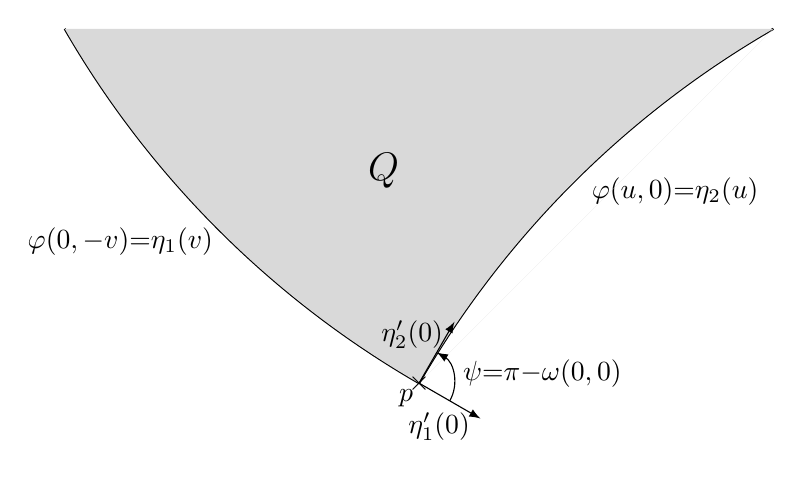
\begin{tikzpicture}[x=.9cm,y=.9cm]
    \pgfmathsetmacro{\cos}{cos(deg(60))}
    \pgfmathsetmacro{\sin}{sin(deg(60))}
    \draw[thick] (0,0) arc[start angle=150,delta angle=-30,radius=13.66] coordinate[pos=0.2] (u1) coordinate[pos=0.4] (u2) coordinate[pos=0.6] (u3) coordinate[pos=0.8] (u4) coordinate[pos=1] (B);
    \coordinate (umid) at (2.3,2.7);
    \draw (umid) node[anchor=west]{$\varphi(u,0){=}\eta_2(u)$};
    \draw[thick] (0,0) arc[start angle=-120,delta angle=-30,radius=13.66] coordinate[pos=0.2] (v1) coordinate[pos=0.4] (v2) coordinate[pos=0.6] (v3) coordinate[pos=0.8] (v4) coordinate[pos=1] (C);

    \path[fill=gray!30] (0,0) arc[start angle=150,delta angle=-30,radius=13.66] (B) -- (C) arc[start angle=-150,delta angle=30,radius=13.66] (0,0);

    \coordinate (vmid) at (-2.9,2.);
    \draw (vmid) node[anchor=east,inner sep=0pt]{$\varphi(0,-v){=}\eta_1(v)$};
 
    \draw[-latex] (0,0) -- (-30:1);
    \draw ($(0,0)+(-45:0.4)$) node[anchor=north]{$\eta_1'(0)$};
    \draw[-latex] (0,0) -- (60:1);
    \draw ($(0,0)+(130:0.9)$) node[anchor=west, inner sep=1pt]{$\eta_2'(0)$};
    \draw[-latex] ($(0,0)+(-30:0.5)$) arc[start angle=-30, delta angle=90, radius=0.5];
    \draw ($(0,0)+(15:0.5)$) node[anchor=west]{$\psi{=}\pi{-}\omega(0,0)$};
    \draw (0,0) node{$\times$};
    \draw (0,0) node[anchor=north east,inner sep=2pt]{$p$};
    \draw (-.5,3.) node{\Large$\sect$};
  \end{tikzpicture}
  \caption{Illustration of a Chebyshev net $\varphi$ on a \\sector $\sect$ of exterior angle $\psi$}\label{fig:sector}
\end{figure}

This theorem gives no information about the regularity of the Chebyshev net, even when the two delimiting curves of the sector are smooth curves. 
Our goal is now to sharpen Theorem \ref{thm:bak-sect} (see Proposition \ref{prop:sector} below) to prove the existence of smooth Chebyshev nets on sectors delimited by smooth curves satisfying the counterpart of \eqref{eq:cond-sector} for smooth curves, namely
\begin{equation}\label{eq:cond-primal}
\int_{\R^+} \ko_2^+ + \int_{\R^-} \ko_1^+ + \int_{\sect} K^+ < \pi-\psi \text{ and } \int_{\R^+} \ko_2^- + \int_{\R^-} \ko_1^- + \int_\sect K^- < \psi.
\end{equation}
To this purpose, we state some preliminary results. First, we relate in Property \ref{prop:geod-curv-c4} the geodesic curvatures of the coordinate curves of Chebyshev nets to the angle $\omega$ between these coordinate curves. Then, we present the Hazzidakis formula in Property \ref{prop:hazz-form}.
See \cite{Ghys09} for a proof of these properties. 
\begin{proprieteE}[Geodesic curvature of coordinate curves]\label{prop:geod-curv-c4}
  Let $\varphi:U\subset\R^2\to\varphi(U)\subset\surf$ be a smooth mapping satisfying \eqref{eq:cheb-def} and let $(u_1,v_1)\in\R^2$ and $(u_2,v_2)\in\R^2$. We denote $\omega:U\to\R/2\pi\Z$ the angle distribution defined by $\omega(u,v) = \angle(\DU\varphi,\DV\varphi)(u,v)$, for all $(u,v)\in U$. Then, supposing $u_1$, $v_1$ and $v_2$ are such that $\{u_1\}\Times[v_1,v_2]\subset U$, we have 
  \begin{equation}\label{eq:courb-geod-v}
    \omega(u_1,v_2) = \omega(u_1,v_1)-\int_{-v_2}^{-v_1}\ko_v,
  \end{equation}
  where $\ko_v:[-v_2,-v_1]\to\R$ is the geodesic curvature of the curve $\eta_1:[-v_2,-v_1]\to\surf$ defined by $\eta_1(v) = \varphi(u_1,-v)$, for all $v\in[-v_2,-v_1]$. This property, illustrated in Figure \ref{fig:parall-transp}, results from the parallel transport of the vector field $\DU\varphi$ along $\eta_1$. Moreover, supposing $u_1$, $u_2$ and $v_1$ are such that $[u_1,u_2]\Times\{v_1\}\subset U$, we have 
  \begin{equation}\label{eq:courb-geod-u}
    \omega(u_2,v_1) = \omega(u_1,v_1)-\int_{u_1}^{u_2}\ko_u,
  \end{equation}
  where $\ko_u:[u_1,u_2]\to\R$ is the geodesic curvature of the curve $\eta_2:[u_1,u_2]\to\surf$ defined by $\eta_2(u) = \varphi(u,v_1)$, for all $u\in[u_1,u_2]$.
\end{proprieteE}
\begin{figure}[!htp]
  \centering
  \begin{tikzpicture}[x=12cm,y=12cm]
    \begin{scope}[decoration={
        markings,
        mark=at position 0.66 with {\arrow{latex}},
        mark=at position 0.33 with {\arrow{latex}}}] 
      \draw[postaction={decorate}] (1,0) to[in=30,out=-130] (0,0);
    \end{scope}
    \pgfmathsetmacro{\r}{.1}
    \pgfmathsetmacro{\RR}{.7*\r}
    \coordinate (A) at (1,0);
    \coordinate (B) at (.65,-.079);
    \coordinate (C) at (.25,.0442);
    \draw (.5,-.08) node{$\varphi(u_1,\cdot)$};
    \draw[thick,->] (A) -- ++(110:\r);
    \draw ($(A)+(45:.07)$) node{\small$~~~~\DU\varphi(u_1,v_1)$};
    \draw[-latex] ($(A)+(110:\RR*.8)$) arc[start angle=110,delta angle=116,radius=\RR*.8];
    \draw ($(A)+(170:\RR+.01)$) node[anchor=east,inner sep=-6pt]{$\omega(u_1,v_1)$};
    \draw[thick,->] (B) -- ++(110:\r);
    \draw (B) node[anchor=south, inner sep=5pt]{\small$~~~~\DU\varphi$};
    \draw[-latex] ($(B)+(110:\RR*.8)$) arc[start angle=110,delta angle=50,radius=\RR*.8];
    \draw ($(B)+(135:\RR+.01)$) node{$\omega$};
    \draw[thick,->] (C) -- ++(110:\r);
    \draw ($(C)+(45:.07)$) node{\small$~~~~\DU\varphi(u_1,v_2)$};
    \draw[-latex] ($(C)+(110:\RR*.8)$) arc[start angle=110,delta angle=70,radius=\RR*.8];
    \draw ($(C)+(160:.12)$) node{$\omega(u_1,v_2)$};
  \end{tikzpicture}
  \vspace{-5.em}
  \caption{Illustration of the parallel transport of $\DU\varphi$ along $\varphi(u_1,\cdot)$}\label{fig:parall-transp}
\end{figure}
\begin{proprieteE}[Hazzidakis formula]\label{prop:hazz-form}
  Let $U = [u_1,u_2]\Times[v_1,v_2]$, with $(u_1,v_1)\in\R^2$ and $(u_2,v_2)\in\R^2$. Let $\varphi : U\to\Omega\subset\surf$, with $\Omega=\varphi(U)$, be a smooth Chebyshev net. We denote $\omega:U\to(0,\pi)$ the angle distribution defined by $\omega=\angle(\partial_u\varphi,\partial_v\varphi)$ and we denote $\eta_1:[-v_2,-v_1]\to\surf$ and $\eta_2:[u_1,u_2]\to\surf$ the two curves respectively defined by $\eta_1(v) = \varphi(u_1,-v)$, for all $v\in[-v_2,-v_1]$, and $\eta_2(u) = \varphi(u,v_1)$, for all $u\in[u_1,u_2]$. We denote $\ko_u:[u_1,u_2]\to\R$ and $\ko_v:[-v_2,-v_1]\to\R$ their respective geodesic curvature. Then, the angle distribution $\omega$ satisfies the following Hazzidakis formula
  \begin{equation}\label{eq:hazz}
    \omega(u_2,v_2) = \omega(u_1,v_1) - \int_{u_1}^{u_2} \ko_u - \int_{-v_2}^{-v_1} \ko_u - \int_{\Omega} K.
  \end{equation}
\end{proprieteE}
\begin{figure}[!htp]
  \captionsetup{justification=centering}
  \begin{center}
    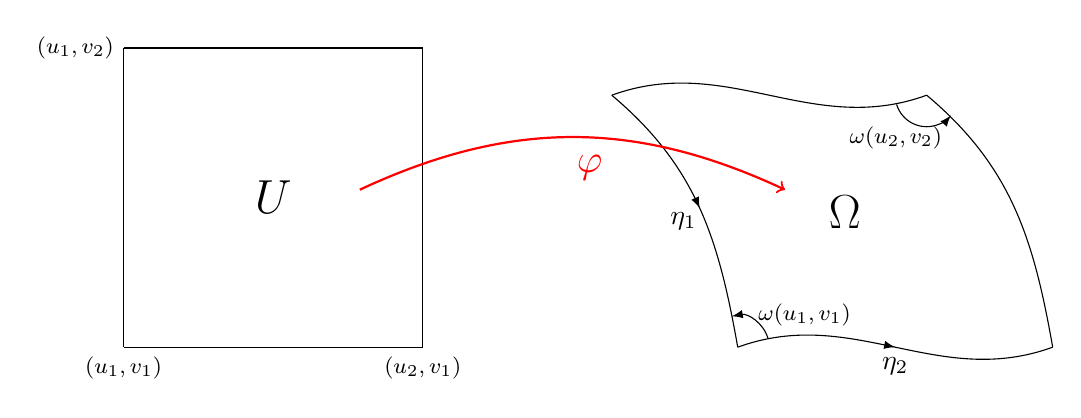
\begin{tikzpicture}[x=4cm,y=4cm]
      \pgfmathsetmacro{\r}{0.1}
      \pgfmathsetmacro{\RR}{.95}
      \begin{scope}[decoration={
        markings,
        mark=at position 0.5 with {\arrow{latex}}}] 
        \draw[postaction={decorate}] (0,0) to[out=20,in=-160] (1,0);
        \draw (1,0) to[out=100,in=-40] (0.6,0.8);
        \draw (0.6,0.8) to[out=-160,in=20] (-0.4,0.8);
        \draw[postaction={decorate}] (-0.4,0.8) to[out=-40,in=100] (0,0);
      \end{scope}

      \draw[-latex] ($(0,0)+(16:\r)$) arc[start angle=16, delta angle=85, radius=\r];
      \draw ($(0,0)+(16:1.3*\r)$) node[anchor=south]{\footnotesize$~~~~~~~\omega(u_1,v_1)$};
      \draw[-latex] ($(0.6,0.8)+(-163:\r)$) arc[start angle=-163, delta angle=123, radius=\r];
      \draw ($(0.6,0.8)+(-145:1.2*\r)$) node[anchor=north]{\footnotesize$\omega(u_2,v_2)$};
%       \draw ($(-0.4,0.8)+(-42:\r)$) arc[start angle=-42, delta angle=59, radius=\r];
      \draw (.34,.43) node{\LARGE$\Omega$};

      \draw (.5,-.06) node{$\eta_2$};
      \draw (-.1,.4) node[anchor=east]{$\eta_1$};

      \coordinate (A) at (-1,0);
      \coordinate (B) at ($(A)+(-\RR,\RR)$);
      \draw (A) -- ++(180:\RR) coordinate (C);
      \draw (A) -- ++(90:\RR);
      \draw (B) -- ++(-90:\RR);
      \draw (B) -- ++(0:\RR);
      \draw (A) node[anchor=north]{\footnotesize$(u_2,v_1)$};
      \draw (C) node[anchor=north]{\footnotesize$(u_1,v_1)$};
      \draw (B) node[anchor=east]{\footnotesize$(u_1,v_2)$};
      \draw[->,red,thick] ($(A)+(-.2,.5)$) to[bend left=25] (.15,.5);
      \draw[red] (-.47,.57) node{\Large$\varphi$};
      \draw ($(A)!.5!(B)$) node{\LARGE$U$};
    \end{tikzpicture}
    \caption{Illustration of the Hazzidakis formula}
    \label{fig:hazz}
  \end{center}
\end{figure}
\begin{lemma}[Homeomorphism]\label{lem:homeo}
  Let $\sect$ be a smooth sector delimited by the two smooth curves $\eta_1:\R^-\to\surf$ and $\eta_2:\R^+\to\surf$ intersecting at $p\in\surf$, and satisfying \eqref{eq:cond-primal}. Assume that $\varphi :(\R^+)^2\to \varphi[(\R^+)^2]\subset\surf$ is a smooth mapping satisfying \eqref{eq:cheb-def}, and such that $\varphi(u, 0) = \eta_2(u)$, $\varphi(0,v) = \eta_1(-v)$ for all $(u,v)\in(\R^+)^2$. Then, $\varphi : (\R^+)^2\to \sect$ is a homeomorphism.
\end{lemma}

\begin{proof}
 The proof is obtained in the same manner as in \cite{Sam95}. We just recall here the principal ideas. We denote $\omega:(\R^+)^2\to\R/2\pi\Z$ the angle distribution defined by $\omega(u,v) = \angle(\DU\varphi,\DV\varphi)(u,v)$, for all $(u,v)\in (\R^+)^2$. We denote $\ko_1:\R^-\to\R$ and $\ko_2:\R^+\to\R$ the geodesic curvatures of $\eta_1$ and $\eta_2$ respectively. First, using \eqref{eq:courb-geod-u}, we obtain that 
\begin{equation*}
  \omega(u,0) = \omega(0,0) - \int_0^u\ko_2 = \pi-\psi-\int_0^u\ko_2,
\end{equation*}
for all $u\in\R^+$. Then, using hypothesis \eqref{eq:cond-primal}, we deduce that $\omega(u,0)\in(0,\pi)$, for all $u\in\R^+$. In the same manner, we obtain that $\omega(0,v) = \pi-\psi-\int_{-v}^0\ko_1\in(0,\pi)$, for all $v\in\R^+$. Hence, using the continuity of $\omega$, we infer that there exists $\tilde D=[0,l_1]\Times[0,l_2]\subset(\R^+)^2$, with $l_1,l_2\in\R^+_\ast$, such that $\omega(\tilde D)\subset(0,\pi)$. Since \eqref{eq:cheb-def} is satisfied, we infer that $\varphi\big|_{\tilde D}:\tilde D\to\varphi(\tilde D)\subset\surf$ is a local homeomorphism, so that, up to reducing $l_1$ and $l_2$, $\varphi$ is a homeomorphism. Moreover, since $\omega(\tilde D)\subset(0,\pi)$, we deduce that $\angle(\eta_2'(u),\DV\varphi(u,0))\in(0,\pi)$, for all $u\in[0,l_1]$, and $\angle(\eta_1'(-v),\DV\varphi(0,v))\in(0,\pi)$, for all $v\in[0,l_2]$. We conclude that, up to reducing $l_1$ and $l_2$, we have $\varphi(\tilde D)\subset \sect$.

Reasoning by contradiction, we first suppose that $\varphi$ is not a homeomorphism. Let $U = [0,L_1)\Times [0,L_2)$ and $U_{\mathrm{cl}} = [0,L_1]\Times [0,L_2]$, with $L_1,L_2>0$,  be such that $\varphi\big|_{U} : U\to \varphi(U)\subset \surf$ is a homeomorphism and such that $\varphi\big|_{U_{\mathrm{cl}}}: U_{\mathrm{cl}}\to\varphi(U_{\mathrm{cl}})\subset\surf$ is not a homeomorphism. Using the Hazzidakis formula \eqref{eq:hazz} and hypothesis \eqref{eq:cond-primal}, we easily obtain that $\omega(U_\mathrm{cl})\subset (0,\pi)$. Hence, the mapping $\varphi\big|_{U_{\mathrm{cl}}}$ is a local homeomorphism.
Now, suppose that there exist $(u_1,v_1),(u_2,v_2)\in(0,L_1]\Times\{L_2\}\cup\{L_1\}\Times(0,L_2]$ with $\varphi(u_1,v_1) = \varphi(u_2,v_2)$. Then, the two following cases are possible:
\begin{itemize}
\item case 1: $u_1=u_2=L_1$ or $v_1=v_2=L_2$. We only consider the first subcase, since the reasoning for the second subcase is similar. Then, assuming that $u_1=u_2=L_1$, one can see that the Gauss--Bonnet formula applied to the curve $\varphi(\{L_1\}\Times[v_1,v_2])$ is in contradiction with \eqref{eq:cond-primal}.
\item case 2: $u_1\neq u_2$ and $v_1\neq v_2$. In this case, we can suppose, without loss of generality, that $v_1=L_2$ and $u_2=L_1$. Then, the Gauss--Bonnet formula applied to the curve $\varphi([u_1,L_1]\Times\{L_2\})\cup\varphi(\{L_1\}\Times[L_2,v_2])$ yields a contradiction with \eqref{eq:cond-primal}.
\end{itemize}
We finally suppose that $\varphi[(\R^+)^2]\not\subset \sect$. Then, let $\tilde U = [0,\tilde L_1)\Times [0,\tilde L_2)$, with $\tilde L_1,\tilde L_2>0$, be such that $\varphi(\tilde U)\subset\sect$ and such that there exists $(\tilde u,\tilde v)\in(0,\tilde L_1]\Times\{\tilde L_2\}\cup\{\tilde L_1\}\Times(0,\tilde L_2]$ with $\varphi(\tilde u,\tilde v)\in\partial \sect$. Then, $\varphi(\tilde u, \tilde v)\in\eta_1(\R^-)$ or $\varphi(\tilde u, \tilde v)\in\eta_2(\R^+)$ and we obtain again a contradiction between the Gauss--Bonnet formula and \eqref{eq:cond-primal}. This concludes the proof.
\end{proof} 

\begin{proposition}[Existence of smooth Chebyshev nets on sectors]\label{prop:sector}
  Let $\sect$ be a smooth sector delimited by the two smooth curves $\eta_1:\R^-\to\surf$ and $\eta_2:\R^+\to\surf$, and with exterior angle $\psi\in(0,\pi)$. Suppose that the geodesic curvatures $\ko_1:\R^-\to\R$ and $\ko_2:\R^+\to\R$ of $\eta_1$ and $\eta_2$ respectively and the Gaussian curvature $K$ of $\sect$ satisfy \eqref{eq:cond-primal}. Then, there exists a unique Chebyshev net $\varphi : (\R^+)^2\to  \sect$ such that
\begin{equation}\label{eq:bound-cond-c4}
\begin{split}
  \varphi(u, 0) &= \eta_2(u), \quad~~\forall u\in\R^+,\\
  \varphi(0,v) &= \eta_1(-v),\quad\forall v\in\R^+.
\end{split}
\end{equation}
Moreover, the angle $\omega=\angle(\partial_u\varphi,\partial_v\varphi)\in(0,\pi)$ of $\varphi$ satisfies the Hazzidakis formula
\begin{equation}\label{eq:hazz2-c4}
\omega(u,v) = \pi - \psi - \int_0^u \ko_2 - \int_{-v}^0 \ko_1 - \int_{\varphi([0,u]\Times[0,v])} K,
\end{equation}
for all $(u,v)\in (\R^+)^2$.
\end{proposition}
The Hazzidakis formula in the sector $\sect$ is illustrated in Figure \ref{fig:hazz2}.

\begin{figure}[!htp]
  \centering
  \begin{tikzpicture}[x=1cm,y=1cm]
    \pgfmathsetmacro{\cos}{cos(deg(60))}
    \pgfmathsetmacro{\sin}{sin(deg(60))}
    \draw[thick] (0,0) arc[start angle=150,delta angle=-30,radius=13.66] coordinate[pos=0.2] (u1) coordinate[pos=0.4] (u2) coordinate[pos=0.6] (u3) coordinate[pos=0.8] (u4);
    \coordinate (umid) at (2.3,2.7);
  %  \draw (umid) node[anchor=west]{$\varphi(u,0){=}\eta_2(u)$};
    \draw[thick] (0,0) arc[start angle=-120,delta angle=-30,radius=13.66] coordinate[pos=0.2] (v1) coordinate[pos=0.4] (v2) coordinate[pos=0.6] (v3) coordinate[pos=0.8] (v4);
    \coordinate (vmid) at (-2.9,2.);
  %  \draw (vmid) node[anchor=east,inner sep=0pt]{$\varphi(0,-v){=}\eta_1(v)$};
   \draw[dotted] (u1) arc[start angle=-120,delta angle=-25,radius=13.66];
   \draw[dotted] (u2) arc[start angle=-120,delta angle=-20,radius=13.66];
   \draw[dotted] (u3) arc[start angle=-120,delta angle=-15,radius=13.66] coordinate[pos=0.8] (uv);
   \draw[dotted] (u4) arc[start angle=-120,delta angle=-10,radius=13.66];
   \draw[dotted] (v1) arc[start angle=150,delta angle=-25,radius=13.66];
   \draw[dotted] (v2) arc[start angle=150,delta angle=-20,radius=13.66];
   \draw[dotted] (v3) arc[start angle=150,delta angle=-15,radius=13.66];
   \draw[dotted] (v4) arc[start angle=150,delta angle=-10,radius=13.66];
   \draw[latex-] ($(uv)+(-42:0.5)$) arc[start angle=-42,delta angle=-96,radius=0.5];
   \draw ($(uv)+(-90:0.5)$) node[anchor=north]{$\omega(u,v)$};
 %   \draw[-latex] (0,0) -- (-30:1);
 %   \draw ($(0,0)+(-45:0.4)$) node[anchor=north]{$\eta_1'(0)$};
 %   \draw[-latex] (0,0) -- (60:1);
 %   \draw ($(0,0)+(130:0.9)$) node[anchor=west, inner sep=1pt]{$\eta_2'(0)$};
  %  \draw[-latex] ($(0,0)+(-30:0.5)$) arc[start angle=-30, delta angle=90, radius=0.5];
 %   \draw ($(0,0)+(15:0.5)$) node[anchor=west]{$\psi{=}\pi{-}\omega(0,0)$};
    \draw (-.5,3.) node{\Large$\sect$};
    \pgfmathsetmacro{\r}{0.5}
    \draw[-latex] (60:\r) arc[start angle=60, delta angle=90, radius=\r];
    \draw ($(90:.7)+(-.2,0)$) node{$\omega(0,0)$};
  \end{tikzpicture}
  \caption{Illustration of the Hazzidakis formula in the sector $\sect$}\label{fig:hazz2}
\end{figure}
Before proving this result, we recall a theorem proved in Chapter \ref{chap4}.
\begin{theorem}[Existence of a unique solution to integrability condition]\label{thm:exist-cond-integr-c5}
Let $\surf$ be a smooth, open, complete, and simply connected surface. Let $\eta_1:\R^-\to\surf$ and $\eta_2:\R^+\to\surf$ be two smooth curves with respective geodesic curvatures $\ko_1:\R^-\to\R$ and $\ko_2:\R^+\to\R$, and such that $\eta_1(0) = \eta_2(0)$. Suppose that $\psi:=\angle(\eta_1'(0),\eta_2'(0))\in(0,\pi)$. Then, there exists a unique angle distribution $\omega:(\R^+)^2\to\R/2\pi\Z$ satisfying the Hazzidakis formula \eqref{eq:hazz2-c4}, with $\varphi:(\R^+)^2\to\surf$ the unique smooth mapping satisfying the boundary conditions \eqref{eq:bound-cond-c4}, and such that its $v$-coordinate curves are arc-length parametrized curves with a geodesic curvature $\kop_2:D\to\R$ satisfying $\kop_2(u,v) = \DV\omega(u,v)$, for all $(u,v)\in (\R^+)^2$.

Suppose moreover that there exists $\tilde D=[0,\tilde L_2]\Times[0,\tilde L_1]$, with $\tilde L_1,\tilde L_2\in\R^+_\ast$, such that $0<\omega(u,v)<\pi$, for all $(u,v)\in \tilde D$. Then, the mapping $\varphi$ satisfies 
\begin{equation}\label{eq:def-cheb3-c5}
  |\DU\varphi|_g(u,v) = |\DV\varphi|_g(u,v)=1,
\end{equation}
for all $(u,v)\in \tilde D$.
\end{theorem}
\begin{proof}[Proof of Proposition \ref{prop:sector}]
  Using Theorem \ref{thm:exist-cond-integr-c5}, we infer that there exists a unique angle distribution $\omega:(\R^+)^2\to\R/2\pi\Z$ satisfying the Hazzidakis formula \eqref{eq:hazz2-c4}, with $\varphi:(\R^+)^2\to\surf$ the unique mapping satisfying the boundary conditions \eqref{eq:bound-cond-c4} and the properties presented in the theorem.
Then, using the continuity of the angle distribution $\omega$ and $\omega(0,0)=\pi-\psi\in(0,\pi)$, we infer that there exists $\tilde L_1,\tilde L_2>0$ such that $\omega(u,v)\in(0,\pi)$ for all $(u,v)\in[0,\tilde L_1]\Times[0,\tilde L_2]$. Hence, by Theorem \ref{thm:exist-cond-integr-c5}, the mapping $\varphi$ satisfies \eqref{eq:def-cheb3-c5} for all $(u,v)\in[0,\tilde L_1]\Times[0,\tilde L_2]$. Then, in the same manner as in the proof of Lemma \ref{lem:homeo}, we obtain that $\varphi:(\R^+)^2\to\sect$ is a Chebyshev net. Suppose finally that $\tilde\varphi:(\R^+)^2\to\surf$ is a Chebyshev net satisfying the boundary conditions \eqref{eq:bound-cond-c4}. Then, using Property \ref{prop:hazz-form}, we obtain that the angle distribution $\tilde\omega:(\R^+)^2\to(0,\pi)$ defined by $\tilde\omega=\angle(\DU\tilde\varphi,\DV\tilde\varphi)(u,v)$, for all $(u,v)\in(\R^+)^2$, satisfies the Hazzidakis formula \eqref{eq:hazz2-c4}. We deduce from Theorem \ref{thm:exist-cond-integr-c5} that $\varphi=\tilde\varphi$. This concludes the proof.
\end{proof}

\subsection{Construction on a broken half-surface}\label{subsubsec:half-surfaces-to-sector}
We now introduce broken half-surfaces which are defined to be half-surfaces with polygonal boundaries:
\begin{definitionE}[(Geodesic) broken half-surfaces]\label{def:n-half-surfaces}
  Let $N\geq 1$ be an integer. We say that $\halfP_c$ is a \emph{broken half-surface} if $\halfP_c$ is a half-surface delimited by a piecewise smooth curve $\gamma:\R\to\surf$ on the partition of $\R$ defined by $-\infty=a_0<...<a_{N+1}=\infty$. We denote $p_i=\gamma(a_i)$, for all $i\in\{1,...,N\}$, and we set $\gamma_i:=\gamma\big|_{[a_{i-1},a_i]}:[a_{i-1},a_i]\to\surf$, for all $i\in\{1,...,N+1\}$. The points $\{p_i\}_{1\leq i\leq N}$ are called the vertices of $\halfP_c$. We suppose moreover that the exterior angle $\psi_i = \angle(\gamma'_{i}(a_i^-), \gamma'_{i+1}(a_i^+))$ at the vertex $p_i$ satisfies $\psi_i\in(0,\pi)$, for all $i\in\{1,...,N\}$. Finally, we define
\begin{equation*}
\psitot=\sum_{1\leq i\leq N}\psi_i,\quad\text{ and }\quad \psim = \max_{1\leq i\leq N}\psi_i
\end{equation*}
and we suppose that $\psitot<\pi$. \emph{Broken half-surfaces} are called geodesic when the boundary curves are geodesic curves. Broken half-surfaces with $N$ vertices are called \emph{$N$-half-surfaces}.
\end{definitionE}
\begin{figure}[!htp]
  \centering
  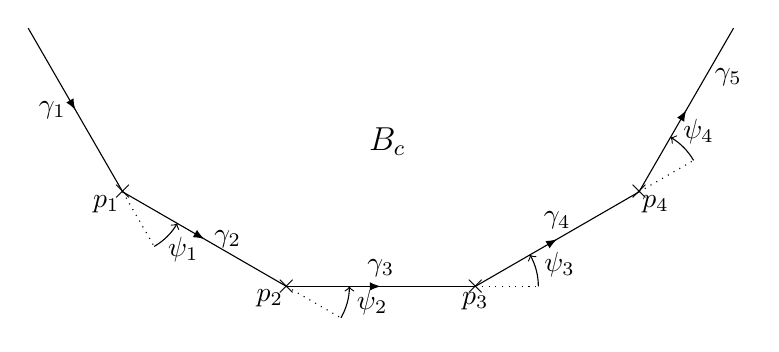
\begin{tikzpicture}[x=0.8cm,y=0.8cm]
    \begin{scope}[decoration={markings,mark=at position 0.5 with {\arrow{latex}}}] 
      \draw[postaction={decorate}] (0,0) coordinate (a0) -- +(-60:3) coordinate[pos=0.5] (g0) coordinate (a1);
      \draw[postaction={decorate}] (a1) -- ($(a1)+(-30:3)$) coordinate[pos=0.5] (g1) coordinate (a2);
      \draw[postaction={decorate}] (a2) -- ($(a2)+(0:3)$) coordinate[pos=0.5] (g2) coordinate (a3);
      \draw[postaction={decorate}] (a3) -- ($(a3)+(30:3)$) coordinate[pos=0.5] (g3) coordinate (a4);
      \draw[postaction={decorate}] (a4) -- ($(a4)+(60:3)$) coordinate[pos=0.7] (g4) coordinate (a5);
    \end{scope}
    \draw (g0) node[anchor=east]{$\gamma_1$};
    \draw[dotted] (a1) -- +(-60:1);
    \draw[->] ($(a1)+(-60:1)$) arc[start angle=-60,delta angle=30,radius=1];
    \draw ($(a1)+(-45:0.8)$) node[anchor=north west]{$\psi_1$};
    \draw (g1) node[anchor=west]{$\gamma_2$};
    \draw[dotted] (a2) -- +(-30:1);
    \draw[->] ($(a2)+(-30:1)$) arc[start angle=-30,delta angle=30,radius=1];
    \draw ($(a2)+(-15:1)$) node[anchor=west]{$\psi_2$};
    \draw (g2) node[anchor=south]{$\gamma_3$};
    \draw[dotted] (a3) -- +(0:1);
    \draw[->] ($(a3)+(0:1)$) arc[start angle=0,delta angle=30,radius=1];
    \draw ($(a3)+(20:1)$) node[anchor=west]{$\psi_3$};
    \draw (g3) node[anchor=south]{$\gamma_4$};

    \draw[dotted] (a4) -- +(30:1);
    \draw[->] ($(a4)+(30:1)$) arc[start angle=30,delta angle=30,radius=1];
    \draw ($(a4)+(60:1.1)$) node[anchor=west]{$\psi_4$};
    \draw (g4) node[anchor=west]{$\gamma_5$};

    \draw (a1) node[anchor=north east, inner sep=1pt]{$p_1$};
    \draw (a2) node[anchor=north east, inner sep=1pt]{$p_2$};
    \draw (a3) node[anchor=north, inner sep=2pt]{$p_3$};
    \draw (a4) node[anchor=north west, inner sep=1pt]{$p_4$};

    \draw (a1) node{$\times$};
    \draw (a2) node{$\times$};
    \draw (a3) node{$\times$};
    \draw (a4) node{$\times$};

    \draw (5.7,-1.8) node{\large$\halfP_c$};
  \end{tikzpicture}
  \caption{Illustration of a geodesic $N$-half-surface $\halfP_c$ with $N=4$}\label{fig:Nhalf-surface}
\end{figure}
We depict the notation introduced in Definition \ref{def:n-half-surfaces} in Figure \ref{fig:Nhalf-surface}. Note that the edges composing $\partial\halfP_c$ are depicted as straight edges in this figure although they are more generally curved edges. We observe that $1$-half-surfaces are smooth sectors. Now, in order to find Chebyshev nets on broken half-surfaces, we view them as sectors delimited by two piecewise smooth curves. This process, called sectorization, is described in the following definition.
\begin{definitionE}[Sectorization]
Let $N\geq1$ and let $\halfP_c$ be a $N$-half-surface delimited by the curves $\{\gamma_i\}_{1\leq i\leq N+1}$. We denote $\{p_i\}_{1\leq i\leq N}$ the vertices of $\halfP_c$. Let $m\in\{1,...,N\}$. We denote $\sect(\halfP_c,p_m)$ the piecewise smooth sector delimited by the curves $\eta_1^m:\R^-\to\surf$ and $\eta_2^m:\R^+\to\surf$ defined so that
\begin{equation}\label{eq:curves-half-surfaces}
\eta^m_1(\R^-) = \bigcup_{i=1}^{m}\gamma_i([a_{i-1},a_{i}]) \quad\text{and}\quad \eta_2^m(\R^+) = \bigcup_{i=m+1}^{N+1}\gamma_i([a_{i-1},a_{i}]).
\end{equation}
\end{definitionE}
The sectorization of a broken half-surface is depicted in Figure \ref{fig:sectorization}.
\begin{figure}[!htp]
  \centering
  \begin{tikzpicture}[x=0.8cm,y=0.8cm]
    \begin{scope}[decoration={markings,mark=at position 0.5 with {\arrow{latex}}}] 
      \draw (0,0) coordinate (a0) -- +(-60:3) coordinate[pos=0.5] (g0) coordinate (a1);
      \draw (a1) -- ($(a1)+(-30:3)$) coordinate[pos=0.5] (g1) coordinate (a2);
      \draw (a2) -- ($(a2)+(0:3)$) coordinate[pos=0.5] (g2) coordinate (a3);
      \draw (a3) -- ($(a3)+(30:3)$) coordinate[pos=0.5] (g3) coordinate (a4);
      \draw (a4) -- ($(a4)+(60:3)$) coordinate[pos=0.7] (g4) coordinate (a5);
    \end{scope}
    \draw (a1) node[anchor=south west]{\large$\eta_1^2$};
    \draw (a4) node[anchor=south east]{\large$\eta_2^2$};

 %   \draw (a1) node[anchor=north east, inner sep=1pt]{$p_1$};
    \draw (a2) node[anchor=north east, inner sep=1pt]{$p_2$};
  %  \draw (a3) node[anchor=north, inner sep=2pt]{$p_3$};
   % \draw (a4) node[anchor=north west, inner sep=1pt]{$p_4$};

   % \draw (a1) node{$\times$};
    \fill (a2) circle (.12);
  %  \draw (a3) node{$\times$};
  %  \draw (a4) node{$\times$};

    \draw (5.7,-1.8) node{\large$\sect(\halfP_c,p_2)$};
  \end{tikzpicture}
  \caption{Illustration of the sectorization $\sect(\halfP_c,p_2)$ of\\ a $N$-half-surface $\halfP_c$ with $N=4$}\label{fig:sectorization}
\end{figure}
We give in the following proposition conditions on $\halfP_c$ for the existence of a sector $\sect(\halfP_c,p_m)$, for some $m\in\{1,...,N\}$, satisfying the conditions \eqref{eq:cond-sector}.

\begin{proposition}[From $N$-half-surfaces to sectors]  \label{prop:half-surface-to-sector}
  Let $N\geq 1$ be an integer. Suppose that the $N$-half-surface $\halfP_c$ satisfies the conditions
  \begin{subequations}\label{eq:cond-half-surface}
    \begin{alignat}{2}  \label{eq:cond-half-surface1}
      \tau_+(\partial \halfP_c) + \int_{\halfP_c} K^+ &< \pi,  \\
      \tau_-(\partial \halfP_c) + \int_{\halfP_c} K^-  &< \psim. \label{eq:cond-half-surface2}
  \end{alignat}
\end{subequations}
Then, there exists $m\in\{1,...,N\}$ such that the piecewise smooth sector $\sect(\halfP_c,p_m)$ satisfies the conditions \eqref{eq:cond-sector}.
\end{proposition}
\begin{proof}
  Let $m = \argmax_{1\leq i\leq N} \psi_i$ and denote $\sect_m = \sect(\halfP_c,p_m)$. Then, a straightforward computation gives
\begin{align*}
\int_{\sect_m} K^+ + \tau_+(\eta_1) + \tau_+(\eta_2) &= \int_{\sect_m} K^+ + \psitot - \psi_m + \sum_{i=1}^{N+1}\int_{a_{i-1}}^{a_{i}}\ko_i^+ =  \tau_+(\partial \halfP_c) + \int_{\halfP_c} K^+ - \psi_m,\\
\int_{\sect_m} K^- + \tau_-(\eta_1) + \tau_-(\eta_2) &= \int_{\sect_m} K^- + \sum_{i=1}^{N+1}\int_{a_{i-1}}^{a_{i}}\ko_i^- <\psi_m.
\end{align*}
Then, conditions \eqref{eq:cond-sector} follow from \eqref{eq:cond-half-surface}.
\end{proof}
\begin{corollaryE}[Existence of Chebyshev nets on $N$-half-surfaces]  \label{cor:cheb-half-surface2}
  Let $N\geq 1$ be an integer. Let $\halfP_c$ be a $N$-half-surface delimited by the curves $(\gamma_i)_{1\leq i\leq N+1}$. Suppose that $\halfP_c$ satisfies the conditions \eqref{eq:cond-half-surface}.
Then, there exist Chebyshev coordinates on $\halfP_c$ such that $(\gamma_i)_{1\leq i\leq N+1}$ are coordinate curves. Moreover, the angle of the net is bounded away from $0$ and $\pi$ by 
\begin{equation}\label{eq:bound-max-angles}
\varepsilon=\min\left(\pi-\tau_+(\partial \halfP_c)-\int_{\halfP_c} K^+,\quad\psim-\tau_-(\partial \halfP_c) - \int_{\halfP_c} K^-\right).
\end{equation}
\end{corollaryE}
\begin{proof}
  The proof follows by combining Proposition \ref{prop:half-surface-to-sector} and Theorem \ref{thm:bak-sect}.
\end{proof}


Finally, in the specific case of geodesic $N$-half-surfaces, we obtain the following theorem:
\begin{theorem}[Existence of Chebyshev nets on geodesic $N$-half-surfaces]\label{thm:cheb-half-surface}
  Let $N\geq 1$. Let $\halfP_c$ be a geodesic $N$-half-surface delimited by the geodesic curves $\{\gamma_i\}_{1\leq i\leq N+1}$. Suppose $\halfP_c$ satisfies the conditions
  \begin{subequations} \label{eq:cond-half-surface-geod}
    \begin{alignat}{2}\label{eq:cond-half-surface-geod1}
      \int_{\halfP_c} K^+ &< \pi-\psitot,\\
      \int_{\halfP_c} K^- &<  \psim.\label{eq:cond-half-surface-geod2}
    \end{alignat}
  \end{subequations}
  Then, there exist Chebyshev coordinates on $\halfP_c$ such that $\{\gamma_i\}_{1\leq i\leq N+1}$ are coordinate curves. Moreover, the angle of the net is bounded away from $0$ and $\pi$ by the positive real number
  \begin{equation}\label{eq:bound-max-angles2}
    \min\left(\pi-\psitot-\int_{\halfP_c} K^+,|\psi|_{l^\infty}-\int_{\halfP_c} K^-\right).
  \end{equation}
\end{theorem}

\section{Splitting of a surface into geodesic broken half-surfaces}\label{subsec:splitting}
In this section, we show how to split any surface $\surf$ satisfying the curvature bound \eqref{eq:cond-thm}
into geodesic broken half-surfaces, each of them satisfying the conditions \eqref{eq:cond-half-surface-geod}. This is the principal result of this section, stated in Theorem \ref{thm:splitting-surf}.
This result is obtained in a similar manner to \cite[Th. 4]{Bur05}: first, we split the surface into four sectors, all of them satisfying \eqref{eq:cond-half-surface-geod1} (see Theorem \ref{thm:burago}). Then, we split recursively each sector into broken half-surfaces, all of them satisfying \eqref{eq:cond-half-surface-geod1} (see Theorem \ref{thm:split}). We finally prove that, after a finite number of splittings, all of the broken half-surfaces also satisfy the condition \eqref{eq:cond-half-surface-geod2}.

\subsection{Splitting of broken half-surfaces}\label{subsubsec:split-half-surfaces}
We prove in this subsection the following theorem which extends the splitting of sectors, introduced in \cite{Bur05}, to broken half-surfaces.
\begin{theorem}[Splitting of $N$-half-surfaces]\label{thm:split}
  Let $N\geq 1$ and let $\halfP_c$ be a $N$-half-surface with exterior angles $\{\psi_i^0\}_{1\leq i\leq N}$ satisfying
\begin{equation} \label{eq:hyp-thm-split}
  \int_{\halfP_c} K^+<\pi-|\psi^0|_{l^1}-2\varepsilon \text{ and } \int_{\halfP_c}K^-<C,
\end{equation}
for positive $C$ and $\varepsilon$. Then, there exist $N_1,N_2\geq 1$ such that 
\begin{equation}\label{eq:nb-vertex}
N_1+N_2\in\{N+1,N+2\}
\end{equation}
and a geodesic curve $\sigma^\ast$ splitting $\halfP_c$ into a $N_1$-half-surface $\halfP_c^1$ with exterior angles $\{\psi_i^1\}_{1\leq i\leq N_1}$ and a $N_2$-half-surface $\halfP_c^2$ with exterior angles $\{\psi_i^2\}_{1\leq i\leq N_2}$ satisfying
\begin{subequations}\label{eq:split}
\begin{alignat}{2}\label{eq:split1}
\int_{\halfP_c^1} K^+ < \pi-|\psi^1|_{l^1}-\varepsilon, &\quad
\int_{\halfP_c^1} K^- < \frac{C}{2}, \\
\int_{\halfP_c^2} K^+ < \pi-|\psi^2|_{l^1}-\varepsilon, &\quad
\int_{\halfP_c^2} K^- < \frac{C}{2},\label{eq:split2}
\end{alignat}
\end{subequations}
with $\displaystyle|\psi^1|_{l^1} = \sum_{i=1}^{N_1}\psi^1_i$, and $\displaystyle|\psi^2|_{l^1} = \sum_{i=1}^{N_2}\psi^2_i$.
\end{theorem}

\begin{remarkE}[$N_1$ and $N_2$]\label{rem:cases-splitting}
Two different cases can happen for the splitting : either the geodesic curve $\sigma^\ast$ intersects $\partial\halfP_c$ at some vertex and we have $N_1+N_2=N+1$, or $\sigma^\ast$ intersects $\partial\halfP_c$ in the interior of some edge and we have $N_1+N_2 = N+2$. See Figure \ref{fig:scheme-splitting-int} for an illustration of these two cases.
\end{remarkE}

\begin{figure}[!htp]
  \begin{center}
    \captionsetup{justification=centering}
    \begin{subfigure}{.5\textwidth}
      \centering
      \begin{tikzpicture}[x=2cm,y=2cm] 
        \draw (0,-3) coordinate (f0) -- +(-60:1) coordinate (f1) -- ($(f1)+(-30:1)$) coordinate (f2) -- ($(f2)+(0:1)$) coordinate (f3) -- ($(f3)+(30:1)$) coordinate (f4) -- ($(f4)+(60:1)$) coordinate (f5);
        % \draw (f1) node[anchor=north]{$a_l$};
        % \draw (f2) node[anchor=south]{$a_{l+1}$};
        \begin{scope}[color=red]
          \draw ($(f1)!0.3!(f2)$) coordinate (f12)   -- ($(f12)+(60:1.55)$) coordinate[pos=0.5] (fmid) 
          node[pos=0.7,anchor=south east, inner sep=1pt]{\large$\sigma^\ast$};
        \end{scope}
        \draw (2.,-3.3) node[anchor=north]{$\halfP_c^1$};
        \draw (0.7,-2.9) node[anchor=north]{$\halfP_c^2$};
      \end{tikzpicture}
      \caption{$\sigma^\ast$ intersects $\partial \halfP_c$ in the interior of some \\ ~~of its edges : $N_1 = 4$ and $N_2 = 2$}
    \end{subfigure}%
    \begin{subfigure}{.5\textwidth}
      \centering
      \begin{tikzpicture}[x=2cm,y=2cm]
        \draw (0,-3) coordinate (f0) -- +(-60:1) coordinate (f1) -- ($(f1)+(-30:1)$) coordinate (f2) -- ($(f2)+(0:1)$) coordinate (f3) -- ($(f3)+(30:1)$) coordinate (f4) -- ($(f4)+(60:1)$) coordinate (f5);
        % \draw (f1) node[anchor=north]{$a_l$};
        % \draw (f2) node[anchor=south]{$a_{l+1}$};
        \begin{scope}[color=red]
          \draw (f2) coordinate (f12)   -- ($(f12)+(75:2)$) coordinate[pos=0.5] (fmid) node[pos=0.7,anchor=south east, inner sep=1pt]{\large$\sigma^\ast$};
        \end{scope}
        \draw (2.5,-3.2) node[anchor=north]{$\halfP_c^1$};
        \draw (1.,-3) node[anchor=north]{$\halfP_c^2$};
      \end{tikzpicture}
      \caption{$\sigma^\ast$ intersects $\partial \halfP_c$ at some of its vertices : \\
        $N_1 = 3$ and $N_2 = 2$}
    \end{subfigure}
    \caption{Illustration of the two possible cases for the splitting in Theorem \ref{thm:split} ($N=4$)}
    \label{fig:scheme-splitting-int}
  \end{center}
\end{figure}
\begin{figure}[!htp]
  \captionsetup{justification=centering}
  \centering
  \begin{tikzpicture}[x=2cm,y=2cm] 
    % Cas (a)
    \begin{scope}[shift={(0.,-0.3)}]
    \draw (0,0) coordinate (b0) -- +(-60:1) coordinate (b1) -- ($(b1)+(-30:1)$) coordinate (b2) -- ($(b2)+(0:1)$) coordinate (b3) -- ($(b3)+(30:1)$) coordinate (b4) -- ($(b4)+(60:1)$) coordinate (b5);
    \begin{scope}[color=red]
      \coordinate (tmp1) at ($(b0)+(30:0.5)$);
      \drawfill[fill=gray!80,opacity=.7] (tmp1) arc[start angle=-150,delta angle=120,radius=1.7] coordinate[pos=0.5] (bmid) \skipit{--} (tmp1);
      
   %   \path[fill=gray!60,opacity=.5] (tmp1) arc[start angle=-150,delta angle=120,radius=1.7] -- (b5) -- (b4) -- (b3) -- (b2) -- (b1) -- (b0) -- ($(b0)+(30:0.5)$);

      \draw[dotted,thick,black] ($(bmid)+(0,0.9)$) -- ($(bmid)+(0,1.3)$);
     % \draw[dotted,thick,black] ($(b0)+(0.2,0.2)$) -- ($(b0)+(0,0.5)$);
     % \draw[dotted,thick,black] ($(b5)+(-0.15,0.2)$) -- ($(b5)+(0,0.5)$);
      
      \draw ($(b0)+(-35:1.2)$) node[anchor=south]{$\sigma(v)$};
      \draw[blue] (bmid) node{$\times$};
      \draw (bmid) node[color=blue,anchor=north west, inner sep=1pt]{$p$};
      \draw[-latex,color=blue] (bmid) -- ($(bmid)+(90:0.5)$) node[anchor=west]{$\theta$};
    \end{scope}
    \draw ($(bmid)+(-0.3,0.4)$) node[anchor=south]{$U(v)$};
 %   \draw ($(b4)+(-0.1,-0.1)$) node[anchor=north]{$U(-v)$};
    \draw ($(b2)!0.5!(b3)$) node[anchor=north,align=left]{\ref{case-a}) $U(v)$ is a half-surface with boundary $\sigma(v)$};
  \end{scope}

  \begin{scope}[shift={(4.,-0.3)}]
    \draw (0,0) coordinate (b0) -- +(-60:1) coordinate (b1) -- ($(b1)+(-30:1)$) coordinate (b2) -- ($(b2)+(0:1)$) coordinate (b3) -- ($(b3)+(30:1)$) coordinate (b4) -- ($(b4)+(60:1)$) coordinate (b5);
    \begin{scope}[color=red]
      \coordinate (tmp1) at ($(b0)+(30:0.5)$);
     % \draw[fill=gray!80,opacity=.7] (tmp1) arc[start angle=-150,delta angle=120,radius=1.7] coordinate[pos=0.5] (bmid) \skipit{--} (tmp1);
      
      \drawfill[fill=gray!60,opacity=.5] (tmp1) arc[start angle=-150,delta angle=120,radius=1.7]  coordinate[pos=0.5] (bmid2) \skipit{--} (b5) \skipit{--} 
      (b4) \skipit{--} (b3) \skipit{--} (b2) \skipit{--} (b1) \skipit{--} (b0) \skipit{--} ($(b0)+(30:0.5)$);

 %     \draw[dotted,thick,black] ($(bmid)+(0,0.9)$) -- ($(bmid)+(0,1.3)$);
      \draw[dotted,thick,black] ($(b0)+(0.2,0.2)$) -- ($(b0)+(0,0.5)$);
      \draw[dotted,thick,black] ($(b5)+(-0.15,0.2)$) -- ($(b5)+(0,0.5)$);
      
      \draw ($(b0)+(-18:1.2)$) node[anchor=south]{$\sigma(v)$};
      \draw[blue] (bmid2) node{$\times$};
      \draw (bmid2) node[color=blue,anchor=south west, inner sep=1pt]{$p$};
  %    \draw[-latex,color=blue] (bmid2) -- ($(bmid2)+(90:0.5)$) node[anchor=west]{$\theta$};
      \draw[-latex,color=blue] (bmid2) -- ++(-90:0.5) node[anchor=west]{$\theta$};
    \end{scope}
%    \draw ($(bmid2)+(-0.3,0.8)$) node[anchor=south]{$U(v)$};
    \draw ($(b4)+(-0.3,0.2)$) node[anchor=north]{$U(v)$};
    \draw ($(b2)!0.5!(b3)$) node[anchor=north,align=left]{\ref{case-b}) $U(v)$ is a polygonal strip};
  \end{scope}
  
    %Cas (c)
\begin{scope}
  \pgfmathsetmacro{\R}{0.4}
    \draw (0,-3) coordinate (f0) -- +(-60:1) coordinate (f1) -- ($(f1)+(-30:1)$) coordinate (f2) -- ($(f2)+(0:1)$) coordinate (f3) -- ($(f3)+(30:1)$) coordinate (f4) -- ($(f4)+(60:1)$) coordinate (f5);
    %\draw (f1) node[anchor=north]{$a_l$};
    %\draw (f2) node[anchor=south]{$a_{l+1}$};

    \draw[dashed] (f4) -- ($(f4)+(30:0.5)$);
    \draw[-latex] ($(f4)+(30:\R)$) arc[start angle=30,
    delta angle=30,radius=\R];
    \draw ($(f4)+(65:\R)$) node[anchor=west]{$~\psi_4^1$};
   \draw[dashed] (f3) -- ($(f3)+(0:0.5)$);
    \draw[-latex] ($(f3)+(0:\R)$) arc[start angle=0,
    delta angle=30,radius=\R];
    \draw ($(f3)+(20:\R)$) node[anchor=west]{$\psi_3^1$};
    \draw[dashed] (f2) -- ($(f2)+(-30:0.5)$) coordinate (qsd);
    \draw[-latex] ($(f2)+(-30:\R)$) arc[start angle=-30,delta angle=30,radius=\R];
    \draw ($(f2)+(-20:\R)$) node[anchor=west]{$\psi_2^1$};

    \begin{scope}[color=red]
      \draw ($(f1)!0.3!(f2)$) coordinate (f12)   -- ($(f12)+(60:1.6)$) coordinate[pos=0.5] 
      (fmid) node[pos=0.5,sloped,blue]{$\times$} node[anchor=south]{$\sigma(v)$};
      \path[fill=gray!80,opacity=.7] (f12) -- ($(f12)+(60:1.6)$) -- (f5)
      -- (f4) -- (f3) -- (f2) -- (f12);
  %    \path[fill,pattern=horizontal lines,pattern color=black] (f12) -- ($(f12)+(60:1.6)$) -- (f0) -- (f1) -- (f12);
      \coordinate (azer) at ($(f12)+(60:1.6)+(-170:.8)$);
    %  \draw[dotted,thick,black] (azer) -- ($(azer)+(110:0.35)$);
      \coordinate (tmp2) at ($(f12)+(60:1.6)+(1,-0.1)$);
      \draw[dotted,thick,black] (tmp2) -- ($(tmp2)+(70:0.35)$);
      
      \draw[dashed] (f12) -- ($(f12)+(-120:0.5)$);
      \draw[-latex] ($(f12)+(-120:0.3)$) arc[start angle=-120,delta angle=90,radius=0.3];
      \draw ($(f12)+(-75:0.27)$) node[anchor=north]{$\psi_1^1$};
      \draw (fmid) node[color=blue,anchor=east]{$p$};
      \draw[-latex,color=blue] (fmid) -- ($(fmid)+(-30:0.5)$) node[anchor=south]{$\theta$};
    %  \draw[-latex,color=blue] (fmid) -- ($(fmid)+(150:0.5)$) node[anchor=west]{$-v$};
    \end{scope}
    \draw ($(f3)+(0.2,1.2)$) node[anchor=north]{$U(v)$};
    \coordinate (tmp3) at ($(f2)!0.5!(f3)$);
    \draw[align=center] ($(tmp3)+(2.,0.25)$) ++(-90:0.5) node[anchor=north]{\ref{case-c}) Both $U(v)$ and $U(-v)$ are broken half-surfaces};
    \end{scope}


\begin{scope}[shift={(4.,0.)}]
  \pgfmathsetmacro{\R}{0.4}
    \draw (0,-3) coordinate (f0) -- +(-60:1) coordinate (f1) -- ($(f1)+(-30:1)$) coordinate (f2) -- ($(f2)+(0:1)$) coordinate (f3) -- ($(f3)+(30:1)$) coordinate (f4) -- ($(f4)+(60:1)$) coordinate (f5);
    %\draw (f1) node[anchor=north]{$a_l$};
    %\draw (f2) node[anchor=south]{$a_{l+1}$};

    \draw[dashed] (f1) -- ++(-60:.5);
    \draw[-latex] ($(f1)+(-60:\R)$) arc[start angle=-60,
    delta angle=30,radius=\R];
    \draw ($(f1)+(-70:\R)$) node[anchor=west]{$~\psi_1^1$};


%    \draw[dashed] (f4) -- ($(f4)+(30:0.5)$);
%    \draw[-latex] ($(f4)+(30:\R)$) arc[start angle=30,
%    delta angle=30,radius=\R];
 %   \draw ($(f4)+(65:\R)$) node[anchor=west]{$~\psi_4^1$};
 %   \draw[dashed] (f3) -- ($(f3)+(0:0.5)$);
 %   \draw[-latex] ($(f3)+(0:\R)$) arc[start angle=0,
 %   delta angle=30,radius=\R];
 %   \draw ($(f3)+(20:\R)$) node[anchor=west]{$\psi_3^1$};
 %   \draw[dashed] (f2) -- ($(f2)+(-30:0.5)$) coordinate (qsd);
 %   \draw[-latex] ($(f2)+(-30:\R)$) arc[start angle=-30,delta angle=30,radius=\R];
 %   \draw ($(f2)+(-20:\R)$) node[anchor=west]{$\psi_2^1$};

    \begin{scope}[color=red]
      \draw ($(f1)!0.3!(f2)$) coordinate (f12)   -- ($(f12)+(60:1.6)$) coordinate[pos=0.5] (fmid) node[pos=0.5,sloped,blue]{$\times$} node[anchor=south]{$\sigma(v)$};
   %   \path[fill,pattern=dots,pattern color=black] (f12) -- ($(f12)+(60:1.6)$) -- (f5)
   %   -- (f4) -- (f3) -- (f2) -- (f12);
      \path[fill=gray!60,opacity=.5] (f12) -- ($(f12)+(60:1.6)$) -- (f0) -- (f1) -- (f12);
      \coordinate (azer) at ($(f12)+(60:1.6)+(-170:.8)$);
      \draw[dotted,thick,black] (azer) -- ($(azer)+(110:0.35)$);
      \coordinate (tmp2) at ($(f12)+(60:1.6)+(1,-0.1)$);
    %  \draw[dotted,thick,black] (tmp2) -- ($(tmp2)+(70:0.35)$);
      
  %    \draw[dashed] (f12) -- ($(f12)+(-120:0.5)$);
      \draw[-latex] ($(f12)+(-30:0.3)$) arc[start angle=-30,delta angle=90,radius=0.3];
      \draw ($(f12)+(5:0.27)$) node[anchor=south west,inner sep=2pt]{$\psi_2^1$};
      \draw (fmid) node[color=blue,anchor=west]{$p$};
%      \draw[-latex,color=blue] (fmid) -- ($(fmid)+(-30:0.5)$) node[anchor=west]{$v$};
      \draw[-latex,color=blue] (fmid) -- ($(fmid)+(150:0.5)$) node[pos=.7,anchor=south,inner sep=3pt]{$\theta$};
    \end{scope}
    \coordinate (tmp3) at ($(f2)!0.5!(f3)$);
 %   \draw[align=center] ($(tmp3)+(0.,0.25)$) ++(-90:0.5) node[anchor=north]{\ref{case-c} The domains $U(v)$ and $U(-v)$ are both\\ broken half-surfaces};
    \end{scope}
    \draw ($(fmid)+(-0.5,-.1)$) node[anchor=north]{$U(v)$};


    %Cas (d) et (e)
\begin{scope}[shift={(-4.,-2.7)}]
  \pgfmathsetmacro{\RR}{0.3}
  \draw (4,-3) coordinate (g0) -- +(-60:1) coordinate (g1) -- ($(g1)+(-30:1)$) coordinate (g2) -- ($(g2)+(0:1)$) coordinate (g3) -- ($(g3)+(30:1)$) coordinate (g4) -- ($(g4)+(60:1)$) coordinate (g5);

  \draw ($(g2)+(-20:\RR)$) node[anchor=west]{\small$\psi_2^1$};
  \draw[dashed] (g4) -- ($(g4)+(30:0.5)$);
  \draw[-latex] ($(g4)+(30:\RR)$) arc[start angle=30,
  delta angle=30,radius=\RR];
  \draw ($(g4)+(75:1.1*\RR)$) node[anchor=west]{\small$~\psi_4^1$};
  \draw[dashed] (g3) -- ($(g3)+(0:0.5)$);
  \draw[-latex] ($(g3)+(0:\RR)$) arc[start angle=0,
  delta angle=30,radius=\RR];
  \draw ($(g3)+(30:\RR)$) node[anchor=west]{\small$\psi_3^1$};
  \draw[dashed] (g2) -- ($(g2)+(-30:0.5)$) coordinate (qsd);
  \draw[-latex] ($(g2)+(-30:\RR)$) arc[start angle=-30,delta angle=30,radius=\RR];
  \begin{scope}[color=red]
    \draw ($(g1)!0.5!(g2)$) coordinate (g12)
    arc[start angle=150,delta angle=-90,radius=1.866] coordinate[pos=0.5] (gmid) coordinate(g45) node[pos=0.8,anchor=south, inner sep=2pt]{$\sigma(v)$};
%    \draw[-latex,color=blue] (gmid) -- ($(gmid)+(105:0.5)$) node[anchor=west]{$-v$};

    \coordinate (azer2) at ($(gmid)+(140:0.45)$);
    %\draw[dotted,thick,black] (azer2) -- ($(azer2)+(90:0.3)$);
    \draw[blue] (gmid) node{$\times$};
    \draw[blue] (gmid) node[anchor=south]{$p$};
    \draw[dashed] (g12) -- ($(g12)+(-120:0.5)$);
   % \draw[dashed] (g45) -- ($(g45)+(-30:0.5)$);
  \end{scope}
    \path[fill=gray!80,opacity=.7] (g12) arc[start angle=150,delta angle=-90,radius=1.866] (g45) -- (g4)
    -- (g3) -- (g2) -- (g12);
    \draw[-latex,color=blue] (gmid) -- ($(gmid)+(-75:0.5)$) node[anchor=west]{$\theta$};

  \draw[red] ($(g12)+(-85:\RR*0.85)$) node{\small$\psi_1^1$};
  \draw[-latex,red] ($(g12)+(-120:\RR/2.)$) arc[start angle=-120,
  delta angle=90,radius=\RR/2.];
  \draw[red] ($(g45)+(90:\RR)$) node{\small$\psi_5^1$};
  \draw[-latex,red] ($(g45)+(60:\RR/2.)$) arc[start angle=60,
  delta angle=90,radius=\RR/2.];

  \draw ($(g1)!0.7!(g4)$) node[anchor=north]{$U(v)$};
 % \draw ($(g1)+(0.3,1.1)$) node[anchor=north]{$U(-v)$};
    
   % \path[fill,pattern=horizontal lines] (g12) arc[start angle=150,delta angle=-90,radius=1.866] (g45) -- (g5)
   % -- (g0) -- (g1) -- (g12);
    \coordinate (tmp4) at ($(g2)!0.5!(g3)$);
    \draw[align=left] ($(tmp4)+(0,0.3)$) ++(-90:0.5) node[anchor=north]{\ref{case-d}) $U(v)$ is a bounded polygonal domain};
\end{scope}

\begin{scope}[shift={(0.,-2.7)}]
  \pgfmathsetmacro{\RR}{0.3}
  \draw (4,-3) coordinate (g0) -- +(-60:1) coordinate (g1) -- ($(g1)+(-30:1)$) coordinate (g2) -- ($(g2)+(0:1)$) coordinate (g3) -- ($(g3)+(30:1)$) coordinate (g4) -- ($(g4)+(60:1)$) coordinate (g5);

%  \draw ($(g2)+(-20:\RR)$) node[anchor=west]{\small$\psi_2^1$};
%  \draw[dashed] (g4) -- ($(g4)+(30:0.5)$);
%  \draw[-latex] ($(g4)+(30:\RR)$) arc[start angle=30,
%  delta angle=30,radius=\RR];
%  \draw ($(g4)+(75:\RR*0.94)$) node[anchor=west]{\small$~\psi_4^1$};
%  \draw[dashed] (g3) -- ($(g3)+(0:0.5)$);
%  \draw[-latex] ($(g3)+(0:\RR)$) arc[start angle=0,
%  delta angle=30,radius=\RR];
%  \draw ($(g3)+(30:\RR)$) node[anchor=west]{\small$\psi_3^1$};
%  \draw[dashed] (g2) -- ($(g2)+(-30:0.5)$) coordinate (qsd);
%  \draw[-latex] ($(g2)+(-30:\RR)$) arc[start angle=-30,delta angle=30,radius=\RR];
  \begin{scope}[color=red]
    \draw ($(g1)!0.5!(g2)$) coordinate (g12)
    arc[start angle=150,delta angle=-90,radius=1.866] coordinate[pos=0.5] (gmid) coordinate(g45) node[pos=0.8,anchor=north, inner sep=2pt]{$\sigma(v)~$};
%    \draw[-latex,color=blue] (gmid) -- ($(gmid)+(-75:0.5)$) node[anchor=west]{$\theta$};
    \draw[-latex,color=blue] (gmid) -- ($(gmid)+(105:0.5)$) node[anchor=west]{$\theta$};

    \coordinate (azer2) at ($(gmid)+(140:0.45)$);
    \draw[dotted,thick,black] (azer2) -- ($(azer2)+(90:0.3)$);
  %  \draw[dashed] (g12) -- ($(g12)+(-120:0.5)$);
    \draw[dashed] (g45) -- ($(g45)+(-30:0.5)$);
      \draw[-latex] ($(g12)+(-30:0.25)$) arc[start angle=-30,delta angle=90,radius=0.25];
      \draw ($(g12)+(-5:0.24)$) node[anchor=south west,inner sep=2pt]{$\psi_2^1$};
      \draw[-latex] ($(g45)+(-30:0.25)$) arc[start angle=-30,delta angle=90,radius=0.25];
      \draw ($(g45)+(-5:0.24)$) node[anchor=south west,inner sep=2pt]{$\psi_3^1$};
      \draw (fmid) node[color=blue,anchor=west]{$p$};
  \end{scope}

%  \draw ($(g12)+(-85:\RR*0.85)$) node{\small$\psi_1^1$};
%  \draw[-latex] ($(g12)+(-120:\RR/2.)$) arc[start angle=-120,
%  delta angle=90,radius=\RR/2.];
%  \draw ($(g45)+(10:\RR*1.3)$) node{\small$\pi{-}\psi_5^1$};
%  \draw[-latex] ($(g45)+(-30:\RR/2.)$) arc[start angle=-30,
%  delta angle=90,radius=\RR/2.];

%  \draw ($(g1)!0.7!(g4)$) node[anchor=north]{$U(v)$};
    
   % \path (g12) arc[start angle=150,delta angle=-90,radius=1.866] (g45) -- (g4)
   % -- (g3) -- (g2) -- (g12);
    \path[fill=gray!60,opacity=.5] (g12) arc[start angle=150,delta angle=-90,radius=1.866] (g45) -- (g5)
    -- (g0) -- (g1) -- (g12);
  \draw ($(g1)+(0.3,.8)$) node[anchor=north]{$U(v)$};
    \draw[blue] (gmid) node{$\times$};
    \draw[blue] (gmid) node[anchor=north]{$p$};
    \coordinate (tmp4) at ($(g2)!0.5!(g3)$);
    \draw[-latex] ($(g1)+(-60:\RR)$) arc[start angle=-60,
    delta angle=30,radius=\RR];
    \draw[dashed] (g1) -- ++(-60:.5);
    \draw ($(g1)+(-70:\RR)$) node[anchor=west]{$~\psi_1^1$};
    \draw[align=center] ($(tmp4)+(0,0.3)$) ++(-90:0.5) node[anchor=north]{\ref{case-e}) $U(v)$ is the complementary of a \\bounded polygonal domain};
\end{scope}
  \end{tikzpicture}
  \caption{Illustration of the possible splittings of a $N$-half-surface \\with $N=4$ (proof of Theorem \ref{thm:split})}\label{fig:splittings}
\end{figure}
\begin{proof}
We adapt the proof of \cite[Thm.3]{Bur05} to $N$-half-surfaces. Let us first recall the setting of this proof. We can assume the metric to be flat outside a compact set $\tilde D\subset \text{int} (\halfP_c)$ homeomorphic to the disk. Moreover, we can suppose that $\tilde D$ is totally convex, i.e., all the geodesic curves joining two points $p,q\in\tilde D$ are included in $\tilde D$. Let $T_p\tilde D$ be the tangent plane at the point $p\in\tilde D$ and let
\begin{equation*}
  S\tilde D = \big\{(p,\theta), \text{ with }p\in \tilde D,~\theta\in T_p\tilde D,~ |\theta|_g=1\big\}
\end{equation*}
be the circle bundle over $\tilde D$.
For any $v=(p,\theta) \in S\tilde D$, we denote $-v=(p,-\theta)$ and $\sigma(v):\R\to\surf$ the unique geodesic curve passing through the point $p$ orthogonally to $v$ (the orientation of $\sigma(v)$ has no importance in what follows). Since $\tilde D$ is totally convex, the geodesic $\sigma(v)$ splits $\tilde D$ into two connected components. The vector $v$ is directed inwards one of these components, which we denote by $U(v)$, and the other component is then denoted $U(-v)$. We now define a function $\alpha$ which plays a similar role to the angular function $\alpha$ in the original proof of \cite[Thm.3]{Bur05}. The continuous function $\alpha:S\tilde D\to [0,\pi]$ should satisfy $\alpha(v)+\alpha(-v)=\pi-|\psi^0|_{l^1}$ for all $v\in S\tilde D$. For this definition, different cases, depicted in Figure \ref{fig:splittings}, have to be considered:
\begin{enumerate}%[label=(\alph*)]
  \item \label{case-a} $U(v)$ is a half-surface with boundary $\sigma(v)$;
  \item \label{case-b} $U(v)$ is a so-called polygonal strip;
  \item \label{case-c} $U(v)$ and $U(-v)$ are respectively a $N_1$-half-surface and a $N_2$-half-surface. We denote $\{\psi_i^1(v)\}_{1\leq i\leq N_1}$ the exterior angles of $\halfP_c^1$ and we set $|\psi^1|_{l^1}:= \sum_{i=1}^{N_1}\psi_i^1(v)$;
  \item \label{case-d} $U(v)$ is a bounded polygonal domain with $N_1$ vertices. We denote $\{\psi_i^1\}_{1\leq i\leq N_1}$ the exterior angles of $U(v)$ and we set $|\psi^1|_{l^1}:=\sum_{i=1}^{N_1}\psi_i^1$;
  \item \label{case-e} $U(v)$ is the complementary of a bounded polygonal domain (so that $U(-v)$ is a bounded polygonal domain).
\end{enumerate}
We emphasize that, for all $v\in\tilde D$, $U(v)$ belongs to one of the above cases. 
Then, we define the function $\alpha$ in each of these cases as follows
\begin{equation}\label{eq:pr-def-alpha}
  \alpha(v)=
  \begin{cases}
    \pi-|\psi^0|_{l^1},&\text{in case \ref{case-a}},\\
    0,&\text{in case \ref{case-b}},\\
    \max\left[\min\left(\pi-|\psi^1|_{l^1},\pi-|\psi^0|_{l^1}\right),0\right],&\text{in case \ref{case-c}},\\
    \max\left[\min\left(2\pi-|\psi^1|_{l^1},\pi-|\psi^0|_{l^1}\right),0\right],&\text{in case \ref{case-d}},\\
    \pi-|\psi^0|_{l^1}-\alpha(-v),&\text{in case \ref{case-e}}.               
  \end{cases}
\end{equation}

Using the continuity of $|\psi^1|_{l^1}$ as $\sigma(v)$ crosses the vertices of $\halfP_c$ and the continuity of all the case transitions, one can check that $\alpha : S\tilde D\to [0,\pi]$ is a continuous function which satisfies $\alpha(-v)+\alpha(v) = \pi-|\psi^0|_{l^1}$. Now, we introduce the mapping $\xi : S\tilde D\to\R^2$ defined by 
\begin{equation*}
\xi(v) = (\xi_1(v),\xi_2(v)) = \left((\pi-|\psi^0|_{l^1}-2\varepsilon)\frac{\int_{U(v)}K^+}{\int_{\tilde D}K^+}-\alpha(v)+\varepsilon,\quad \frac{\int_{U(v)}K^-}{\int_{\tilde D}K^-}-\frac{1}{2}\right).
\end{equation*}
Then, $\xi_1$ satisfies
\begin{align*}
  \xi_1(-v) &= (\pi-|\psi^0|_{l^1} -2\varepsilon)\frac{\int_{\tilde D}K^+ - \int_{U(v)}K^+}{\int_{\tilde D}K^+} - \alpha(-v) + \varepsilon\\
  &= \pi-|\psi^0|_{l^1} -2\varepsilon - (\pi-|\psi^0|_{l^1} -2\varepsilon)\frac{\int_{U(v)}K^+}{\int_{\tilde D}K^+} - (\pi-|\psi^0|_{l^1} - \alpha(v)) + \varepsilon\\
  &= -\xi_1(v).
\end{align*}
In the same manner, we obtain that $\xi_2(-v) = -\xi_2(v)$, so that $\xi(-v) = -\xi(v)$.
Therefore, using \cite[Prop. 1]{Bur05}, we can conclude that there exists $v_0\in S\tilde D$ such that $\xi(v_0) = (0,0)$, which corresponds to
\begin{equation}\label{eq:pr-split-Nhalf}
  \alpha(v_0) = (\pi-|\psi^0|_{l^1}-2\varepsilon)\frac{\int_{U(v_0)}K^+}{\int_{\tilde D}K^+}+\varepsilon,
\quad\int_{U(v_0)} K^- = \frac{1}{2}\int_{\tilde D} K^-.
\end{equation}
 We now prove that $U(v_0)$ necessarily matches case \ref{case-c}. First, by \eqref{eq:pr-split-Nhalf}, we have 
\begin{equation}\label{eq:pr-split-Nhalf2}
\alpha(v_0)\in[\varepsilon,\pi-|\psi^0|_{l^1}-\varepsilon],
\end{equation}
which rules out cases \ref{case-a} and \ref{case-b}. In order to rule out cases \ref{case-d} and \ref{case-e}, suppose now that $U(v)$ is a bounded polygonal domain. Applying the Gauss--Bonnet formula on $U(v)$, we infer that
\begin{equation*}
  |\psi^1|_{l^1}+\int_{U(v)}K = 2\pi,
\end{equation*}
which gives $2\pi - |\psi^1|_{l^1} \leq \int_{U(v_0)} K^+$. Then, using the hypotheses \eqref{eq:hyp-thm-split} and \eqref{eq:pr-split-Nhalf}, we obtain that
\begin{equation}\label{eq:pr-split-Nhalf3}
\int_{U(v_0)}{K^+}+\varepsilon < \alpha(v_0).
\end{equation}
Combining these two results and the definition of $\alpha$ in case \ref{case-d}, we obtain the following contradiction:
\begin{equation*}
  2\pi-|\psi^1|_{l^1}\leq \int_{U(v_0)}{K^+} < \alpha(v_0)-\varepsilon \leq 2\pi-|\psi^1|_{l^1}-\varepsilon.
\end{equation*}
Finally, if $U(v_0)$ matches case \ref{case-e}, then $\xi(-v_0)=0$. Hence, $U(-v_0)$ matches case \ref{case-d} which leads, as above, to a contradiction.
Therefore $U(v_0)$ necessarily matches case \ref{case-c}, i.e., both $U(v_0)$ and $U(-v_0)$ are broken half-surfaces. Moreover, \eqref{eq:pr-def-alpha} and \eqref{eq:pr-split-Nhalf2} show that $\alpha(v_0) = \pi-|\psi^1|_{l^1}$. Then, using \eqref{eq:pr-split-Nhalf} and \eqref{eq:pr-split-Nhalf3}, we infer that \eqref{eq:split} is satisfied by $U(v_0)$. Since $\xi(-v_0)=0$, we obtain, by symmetry, the same result for $U(-v_0)$. Finally, recalling Remark \ref{rem:cases-splitting}, we have $N_1+N_2\in\{N+1,N+2\}$. This concludes the proof.
\end{proof}

\comment{
\begin{remarkE}
Note that, as in \eqref{eq:res-burago}, in order to minimize the number of $N$-half-surfaces in the final step of the proof, it would be necessary to take into account the angle between $\sigma$ and the boundary of $\halfP_c$ in \eqref{eq:split}.
\end{remarkE}
}

\subsection{Recursive splitting}\label{subsubsec:rec-split}
We first restate a result by Burago \textit{et al} \cite[Theorem 3]{Bur05} that allows one to split surfaces satisfying
\begin{equation}    \label{eq:cond-burago}
  \int_\surf K^+ < 2\pi - 4\varepsilon,\quad\text{ and }\quad \int_\surf K^- < C-4\varepsilon,
\end{equation}
for positive $C$ and $\varepsilon$, into four sectors delimited by geodesic curves, all of them satisfying the condition \eqref{eq:cond-half-surface-geod1}. This result is stated in \cite{Bur05} with $C=2\pi$, but the proof is valid in the general setting. 
\begin{theorem}[Burago {\it et al.}]\label{thm:burago}
    Let $\surf$ be a complete Riemannian 2-manifold homeomorphic to the plane and satisfying the conditions \eqref{eq:cond-burago}, for positive $C$ and $\varepsilon$. Then, there exist four sectors $\{\sect_i\}_{1\leq i\leq 4}$ with exterior angles $\{\psi_i\}_{1\leq i\leq 4}$ and delimited by geodesic curves such that $\text{int}(\sect_i)\cap \text{int}(\sect_j) = \varnothing$ for all $i \neq j$ and $\cup_{1\leq i\leq 4} \sect_i = \surf$, and such that, for all $i\in\{1,...,4\}$, the sector $\sect_i$ satisfies the conditions
\begin{equation}\label{eq:res-burago}
\int_{\sect_i} K^+ \leq \pi - \psi_i-\varepsilon,\quad \int_{\sect_i} K^- \leq \frac{C}{2\pi}\psi_i-\varepsilon.
\end{equation}
\end{theorem}
The four sectors obtained by this theorem are sketched in Figure \ref{fig:scheme-thm-burago}.
\begin{figure}[!htp]
  \centering
  \begin{tikzpicture}[x=0.3cm,y=0.3cm]
    \pgfmathsetmacro{\R}{0.7}
    \pgfmathsetmacro{\RR}{1.4}
    \coordinate (A) at (-8,0);
    \coordinate (B) at (3,0);
    \coordinate (B2) at (14,0);

    \coordinate (C) at ($(B)+(60:6)$);

    \draw (A) -- (B) coordinate[pos=0.5] (AA);
    \draw[dashed] (A) -- ($(A)+(-3,0)$);
    \draw (B) -- (B2) coordinate[pos=0.5] (BB);

    \coordinate (Z) at ($(BB)+(-1.,-3)$);
    \coordinate (Z2) at ($(BB)+(-2.,-6.)$);

    \draw[dashed] (B2) -- ($(B2)+(4,0)$);
    \draw (B) -- (C);
    \draw[dashed] (C) -- ($(C)+(60:2)$);
    \draw (BB) -- (Z2);
    \draw[dashed] (Z2) -- ($(Z2)+(-0.5,-1.5)$);

    \draw (-3,5) node{\Large$\sect_2$};
    \draw (10,4.3) node{\Large$\sect_1$};
    \draw (1.8,-3.8) node{\Large$\sect_3$};
    \draw (12,-3.8) node{\Large$\sect_4$};
  \end{tikzpicture}
  \caption{Illustration of the splitting of Theorem \ref{thm:burago}}  \label{fig:scheme-thm-burago}
\end{figure}
 We also need the following lemma to bound from below the exterior angles of the broken half-surfaces resulting from splitting:
\begin{lemma}[Bound on exterior angles]  \label{lem:bound-angles}
  Let $N\geq1$ and let $\halfP_c$ be a $N$-half-surface satisfying the condition \eqref{eq:cond-half-surface-geod1}.
  Let $\sigma : \R^+\to \halfP_c$ be a geodesic curve with $\sigma(0)\in\partial \halfP_c$ and suppose that $\sigma$ splits $\halfP_c$ into a $N_1$-half-surface $\halfP_c^1$ and a $N_2$-half-surface $\halfP_c^2$, both of which satisfy the condition \eqref{eq:cond-half-surface-geod1}. Then, denoting $\{\psi^0_k\}_{1\leq k\leq N}$, $\{\psi_k^1\}_{1\leq k\leq N_1}$, and $\{\psi_k^2\}_{1\leq k\leq N_2}$, the positive exterior angles of $\halfP_c$, $\halfP_c^1$, and $\halfP_c^2$, respectively, we have 
  \begin{equation}\label{eq:bound-angles}
    \forall i\in\{1,2\},\quad|\psi^i|_{l^\infty}\geq|\psi^0|_{l^\infty}.
  \end{equation}
\end{lemma}
\begin{proof}
  We denote $\psi_k^1$, with $k\in\{1,...,N_1\}$, and $\psi_l^2$, with $l\in\{1,...,N_2\}$, the exterior angle of $\halfP_c^1$ and $\halfP_c^2$ respectively at the intersection of $\sigma$ with $\partial \halfP_c$. Two cases can occur: either the intersection point is not located at some vertex of $\partial \halfP_c$, or $\sigma$ intersects a vertex $p_n\in\partial \halfP_c$, with $n\in\{1,...,N\}$, with exterior angle $\psi^0_n$ (see Remark \ref{rem:cases-splitting} and Figure \ref{fig:scheme-splitting-int}). In the first case, we have $\psi_k^1+\psi_l^2=\pi$. In the second case, since $\psi^0_n\geq 0$, we have $\psi_k^1+\psi_l^2=\pi+\psi^0_n\geq\pi$. In both cases, we infer that
  \begin{equation}\label{eq:split-bound}
    \psi_k^1+\psi_l^2\geq\pi.
  \end{equation}
  Note that all the angles of both $\halfP_c^1$ and $\halfP_c^2$ are angles of $\halfP_c$, except for the angle newly created by the intersection of $\sigma$ with $\partial \halfP_c$. Let $\psi^0_m$, with $m\in\{1,...,N\}$, be an exterior angle of $\halfP_c$ such that $\psi^0_m=|\psi^0|_{l^\infty}$. Let $p_m$ be the corresponding vertex of $\partial\halfP_c$. We only prove that \eqref{eq:bound-angles} is satisfied for $i=1$, since the case $i=2$ is treated similarly. We remark that three cases can occur:
  \begin{enumerate}%[label=(\alph*)]
  \item If $p_m$ is contained in $\halfP_c^1$, the result is straightforward;
  \item If $p_m$ is contained in $\halfP_c^2$, applying \eqref{eq:split-bound} and the condition \eqref{eq:cond-half-surface-geod1} in $\halfP_c^1$, we obtain that
    \begin{equation*}
      \psi_k^1\geq \pi-\psi_l^2 \geq |\psi^0|_{l^1} - \psi^2_l+\int_{\halfP_c^2}{K^+} \geq \psi^0_m.
    \end{equation*}
  \item Finally, if $\sigma$ intersects $\partial\halfP_c$ at $p_m$, we have $\psi_k^1+\psi_l^2=\pi+\psi^0_m$. Since $\psi_l^2\leq \pi$, we infer that $\psi_k^1\geq\psi^0_m$.
  \end{enumerate}
In all the cases, we obtain the expected result. This concludes the proof.
\end{proof}
We can now prove the main result of this section.
\begin{theorem}[Surface splitting into broken half-surfaces]\label{thm:splitting-surf}
  Let $\surf$ be a smooth, complete, simply connected surface. Suppose that $\surf$ satisfies the curvature bound \eqref{eq:cond-thm}, i.e.,
\begin{equation*}% \label{eq:cond-thm2}
  \int_{\surf}K^+<2\pi\quad\text{and}\quad\int_{\surf}K^-<\infty,
\end{equation*} 
with $K$ the Gaussian curvature of $\surf$, $K^+=\max(K,0)$ and $K^-=\max(-K,0)$. We set $n_{\max}:=\log_2\left(\frac{1}{\pi}\int_\surf K^-+1\right)+2$. Then, there exist $\Npol\leq \frac{4}{\pi}\int_\surf K^-+8$ geodesic $N_{\alpha}$-half-surfaces $\{\halfP_c^\alpha\}_{1\leq\alpha\leq\Npol}$, with $N_\alpha\leq n_{\max}$ for all $\alpha\in\{1,...,\Npol\}$, satisfying the conditions \eqref{eq:cond-half-surface-geod} and such that $\mathrm{int}(\halfP_c^\alpha)\cap \mathrm{int}(\halfP_c^\beta)=\varnothing$ for all $\alpha\neq\beta$ and $\surf = \cup_{\alpha=1}^{\Npol} \halfP_c^{\alpha}$.
\end{theorem}
\begin{proof}
Let $\bar\varepsilon = \frac{1}{5}\big(2\pi-\int_{\surf}K^+\big)$ and $\bar C = \int_\surf K^- + 5\bar\varepsilon$. Then, the hypotheses of Theorem \ref{thm:burago} are satisfied by $\surf$ with $\varepsilon = \bar\varepsilon$ and $C=\bar C$. We denote $\{\HalfP_{\alpha,0}\}_{1\leq \alpha\leq 4}$ the four sectors satisfying \eqref{eq:res-burago} obtained by this theorem. 
As condition \eqref{eq:cond-half-surface-geod1} is satisfied by each $1$-half-surface $\HalfP_{\alpha,0}$ the proof consists in applying multiple times Theorem \ref{thm:split} to all of them so as to split these $1$-half-surfaces recursively until condition \eqref{eq:cond-half-surface-geod2} on the total negative curvature is satisfied. Since each broken half-surface is treated similarly, we only enumerate one broken half-surface in each sector $\HalfP_{\alpha,0}$ at each step of the subdividision. (Note that, otherwise, multi-indices should have been introduced.)
See Figure \ref{fig:subd} for an illustration of the resulting splitting. We denote, for all $\alpha\in \{1,...,4\}$, $\psi_\alpha>0$ the exterior angle of $\HalfP_{\alpha,0}$ and we set $C_{\alpha}=\frac{\bar C\psi_\alpha}{2\pi}$. Since $\HalfP_{\alpha,0}$ satisfies \eqref{eq:res-burago}, the hypotheses of Theorem \ref{thm:split} are satisfied with $\halfP_c=\HalfP_{\alpha,0}$, $\varepsilon = \frac{\bar\varepsilon}{3}$ and $C=C_{\alpha}$. Hence, there exists a splitting of $\HalfP_{\alpha,0}$ into two broken half-surfaces satisfying the conditions \eqref{eq:split}. By symmetry, we consider only one of them, denoted $\HalfP_{\alpha,1}$. In the same manner, we apply recursively Theorem \ref{thm:split} with $\halfP_c = \HalfP_{\alpha,n-1}$, $\varepsilon = \frac{\bar\varepsilon}{3.2^{n-1}}$ and $C=\frac{C_\alpha}{2^{n-1}}$. This yields a splitting of $\HalfP_{\alpha,n-1}$ into two broken half-surfaces satisfying the conditions \eqref{eq:split}. By symmetry, we consider only one of them, the $N$-half-surface denoted $\HalfP_{\alpha,n}$, whose exterior angles are denoted $\{\psi^n_k\}_{1\leq k\leq N}$.
Note that $N\leq n+1$ by \eqref{eq:nb-vertex}. Then, Lemma \ref{lem:bound-angles} ensures that $|\psi^n|_{l^\infty}\geq \psi_\alpha$ (with $|\psi^n|_{l^\infty} = \max_{1\leq k\leq N}\psi_k^n$). Therefore, condition \eqref{eq:cond-half-surface-geod2} is satisfied by $\HalfP_{\alpha,n}$ whenever
\begin{equation}\label{eq:pr-splitting-surf}
\int_{\HalfP_{\alpha,n}}K^-< |\psi^n|_{l^\infty} \leq \psi_\alpha.
\end{equation}
Since $\int_{\HalfP_{\alpha,n}}K^-\leq \frac{C_\alpha}{2^n}$, we infer that \eqref{eq:pr-splitting-surf} is satisfied whenever $n=n_\alpha^{\max}$, where
\begin{equation*}
  n^{\mathrm{max}}_\alpha = \left\lceil\log_2\left(\frac{C_\alpha}{\psi_\alpha}\right)\right\rceil = \left\lceil\log_2\left(\frac{\bar C}{2\pi}\right)\right\rceil
\end{equation*}
and $\lceil\cdot\rceil$ is the ceiling function. Therefore, we have proved that there exist $\N_\alpha$ $N_i$-half-surfaces $\{\halfP_c^{\alpha,i}\}_{1\leq i\leq \N_\alpha}$, with $N_i\leq n^{\mathrm{max}}_\alpha+1$, such that $\mathrm{int}(\halfP_c^{\alpha,i})\cap \mathrm{int}(\halfP_c^{\alpha,j}) = \varnothing$ for all $i\neq j$. Moreover, we have $\N_\alpha\leq\N_\alpha^{\max}$, with:
\begin{equation}\label{eq:pr-splitting-surf2}
  \N_\alpha^{\max}=2^{n_\alpha^{\max}}\leq \frac{\bar C}{\pi}\leq \frac{1}{\pi}\int_\surf K^-+2.
\end{equation}
We finally define $\Npol = \sum_{\alpha=1}^4\N_\alpha$ and the set of $N_i$-half-surfaces $\{\halfP^i_c\}_{1\leq i\leq\Npol}$ as the union of the sets $\{\halfP_c^{\alpha,i}\}_{1\leq i\leq\N_\alpha}$, for $\alpha\in\{1,...,4\}$. For all $i\in\{1,...,\Npol\}$, the number $N_i$ of vertices of $B^i_c$ satisfies
\begin{align*}
N_i&\leq \max_{\alpha\in\{1,...,4\}}n^{\mathrm{max}}_\alpha+1=\left\lceil\log_2\left(\frac{\bar C}{2\pi}\right)\right\rceil+1\\
& \leq \log_2\left(\frac{1}{2\pi}\int_\surf K^-+1\right)+2=n_{\max}.
\end{align*}
Moreover, using \eqref{eq:pr-splitting-surf2}, we obtain that the number $\Npol$ of polygons satisfies
\begin{equation*}
  \Npol=\sum_{\alpha=1}^4\N_\alpha\leq \frac{4}{\pi}\int_\surf K^-+8.
\end{equation*}
The claim follows. %Once the subdividision is achieved, we number the 
\end{proof}
\begin{figure}[!htp]
  \centering
  \def\sizef{0.4cm}
    \begin{subfigure}{\textwidth}
      \begin{center}
        \begin{tikzpicture}[x=\sizef,y=\sizef]
          \schemSubd
          \draw (-3,5) node{\Large$\HalfP_{2,0}$};
          \draw (10,4.3) node{\Large$\HalfP_{1,0}$};
          \draw (1.8,-3.8) node{\Large$\HalfP_{3,0}$};
          \draw (12,-3.8) node{\Large$\HalfP_{4,0}$};
        \end{tikzpicture}
        \caption{$1^{\text{st}}$ step: splitting of $\surf$ into $4$ sectors}
      \end{center}
    \end{subfigure}
    
   \begin{subfigure}{\textwidth}
      \begin{center}
        \begin{tikzpicture}[x=\sizef,y=\sizef]
          \schemSubd
          \draw (11.5,4.3) node{\large$\HalfP_{1,1}$};
          \draw (0,5) node{\large$\HalfP_{2,1}$};
          \draw (-1.,-3.) node{\large$\HalfP_{3,1}$};
           \draw (Z) -- (Y);
           \draw[dashed] (Y) -- ($(Y)+(-2.,-0.66)$);
           \draw (AA) -- (AAB);
           \draw (AAB) -- (AAB2);
           \draw[dashed] (AAB2) -- ($(AAB2)+(-0.75,2.)$);
           \draw (C) -- (D);
           \draw (D) -- (D2);
           \draw[dashed] (D2) -- ($(D2)+(1,1)$);
         \end{tikzpicture}
        \caption{$2^{\text{nd}}$ step: splitting of $\{\HalfP_{\alpha,0}\}_{1\leq\alpha\leq 4}$}
       \end{center}
    \end{subfigure}
    
   \begin{subfigure}{\textwidth}
     \begin{center}
       \begin{tikzpicture}[x=\sizef,y=\sizef]
         \schemSubd
         \draw (11.,6.3) node{\large$\HalfP_{1,2}$};
          \draw (0,5) node{\large$\HalfP_{2,2}$};
         \draw (Z) -- (Y);
         \draw[dashed] (Y) -- ($(Y)+(-2.,-0.66)$);
         \draw (AAB) -- (AAC);
         \draw[dashed] (AAC) -- ($(AAC)+(0,2.)$);\draw (AA) -- (AAB);
         \draw (AAB) -- (AAB2);
         \draw[dashed] (AAB2) -- ($(AAB2)+(-0.75,2.)$);
         \draw (C) -- (D);
         \draw (D) -- (D2);
         \draw[dashed] (D2) -- ($(D2)+(1,1)$);
         \draw (D) -- (E);
         \draw (E) -- (E2);
         \draw[dashed] (E2) -- ($(E2)+(2.5,0.5)$);
       \end{tikzpicture}
       \caption{$3^{\text{rd}}$ step: splitting of $\{\HalfP_{\alpha,1}\}_{1\leq\alpha \leq4}$}
      \end{center}
    \end{subfigure}
  \caption{Illustration of the recursive splitting used for \\the proof of Theorem \ref{thm:splitting-surf}}  \label{fig:subd}
\end{figure}
\begin{remarkE}[Tree representation]\label{rem:binary-tree}
  The construction can be seen as a binary tree of broken half-surfaces, each splitting being an edge, $n_{\max}$ being the maximal depth of the tree, and $\Npol$ being the maximal number of leaves of the tree. Once the splitting is achieved, we renumber the broken half-surfaces to obtain the set $\{\halfP_c^\alpha\}_{1\leq\alpha\leq\Npol}$.
\end{remarkE}
\begin{definitionE}[Skeleton]
  The graph in the surface $\surf$ defined by the vertices of the boundaries of the broken half-surfaces $\{\halfP^\alpha_c\}_{1\leq\alpha\leq\Npol}$ obtained using Theorem \ref{thm:splitting-surf} and the edges (geodesic curves) joining the vertices is called the \emph{skeleton}. The vertices and the edges in the \emph{skeleton} are respectively enumerated as $\{p_c^i\}_{1\leq i\leq \Nver}$ and $\{\gamma_c^i\}_{1\leq i\leq \Ned}$.
\end{definitionE}
An example of skeleton is then presented in Figure \ref{fig:skeleton}.
\begin{figure}[!htp]
  \centering
  \begin{tikzpicture}[x=0.6cm,y=0.6cm]
    \pgfmathsetmacro{\R}{0.7}
    \pgfmathsetmacro{\RR}{1.4}
    \coordinate (A) at (-8,0);
    \coordinate (B) at (3,0);
    \coordinate (B2) at (14,0);

    \coordinate (C) at ($(B)+(0.66,2)$);
    \coordinate (C2) at ($(B)+(2.25,6.75)$);
    \coordinate (D) at ($(C)+(2,2)$);
    \coordinate (D2) at ($(C)+(5,5)$);
    \coordinate (E) at ($(D)+(5,1)$);
    \coordinate (E2) at ($(D)+(8.75,1.75)$);

    \draw (A) -- (B) coordinate[pos=0.5] (AA);
    \draw[dashed] (A) -- ($(A)+(-3,0)$);
    \draw (B) -- (B2) coordinate[pos=0.5] (BB) node[pos=0.8,anchor=north,inner sep=2pt]{$\gamma^1_c$} 
    node[pos=0.2,anchor=north,inner sep=2pt]{$\gamma^2_c$};

    \coordinate (Z) at ($(BB)+(-1.,-3)$);
    \coordinate (Z2) at ($(BB)+(-2.,-6.)$);
    \coordinate (Y) at ($(Z)+(-9,-3)$);
    \coordinate (AAB) at ($(AA)+(-1.5,3.)$);
    \coordinate (AAB2) at ($(AAB)+(-1.5,3.)$);
    \coordinate (AAC) at ($(AAB)+(0,3.5)$);

    \draw[dashed] (B2) -- ($(B2)+(4,0)$);
    \draw (B) -- (C) node[pos=0.5,anchor=east,inner sep=2pt]{$\gamma^3_c$};
    \draw (C) -- (C2);
    \draw[dashed] (C2) -- ($(C2)+(0.5,1.5)$);
    \draw (C) -- (D) node[pos=0.5,anchor=north west,inner sep=-1pt]{$\gamma^4_c$};
    \draw (D) -- (D2) node[pos=0.8,anchor=north west,inner sep=-2pt]{$\gamma^6_c$};
    \draw[dashed] (D2) -- ($(D2)+(1,1)$);
    \draw (D) -- (E) node[pos=1.,anchor=north west,inner sep=-1pt]{$\gamma^5_c$};
    \draw (E) -- (E2);
    \draw[dashed] (E2) -- ($(E2)+(2.5,0.5)$);

    \draw (BB) -- (Z);
    \draw (Z) -- (Z2) node[pos=.7,anchor=north west,inner sep=-1pt]{$\gamma^{\Ned}_c$};
    \draw[dashed] (Z2) -- ($(Z2)+(-0.5,-1.5)$);
    \draw (Z) -- (Y);
    \draw[dashed] (Y) -- ($(Y)+(-2.,-0.66)$);

    \draw (AA) -- (AAB);
    \draw (AAB) -- (AAB2);
    \draw[dashed] (AAB2) -- ($(AAB2)+(-0.75,2.)$);
    \draw (AAB) -- (AAC);
    \draw[dashed] (AAC) -- ($(AAC)+(0,2.)$);

  %  \draw[very thin,-latex] (B)++(0:\R) arc (0:70:\R);
  %  \draw (B)++(30:2.5*\R) node{$\psi_l {=} \psi^1_3$};

 %   \draw[very thin,-latex] (AA)++(0:\R) arc (0:115:\R);
 %   \draw (AA)++(60:2.*\R) node{$\psi^3_1$};
 %   \draw[very thin,latex-] (AA)++(180:1.2*\R) arc (180:115:1.2*\R);
 %   \draw (AA)++(145:2.*\R) node{$\psi^1_2$};

  %  \draw[very thin,-latex] (AAB)++(-60:\R) arc (-60:90:\R);
  %  \draw (AAB)++(20:1.7*\R) node{$\psi^2_1$};

 %   \draw[very thin,-latex] (AAB)++(90:2.*\R) arc (90:118:2.*\R);
 %   \draw (AAB)++(105:3.*\R) node{$\psi^1_1$};


 %   \draw (0,5) node{\Large$\halfP^4$};
    \draw (6.4,6.5) node{\large$\halfP^3_c$};
    \draw (11.5,3.) node{\large$\halfP^1_c$};
    \draw (11.,6.3) node{$\halfP^2_c$};
  %  \draw (11,6.5) node{$\HalfP^{\text{right}}_{1,2}$};
  %  \draw (11,2.3) node{\large$\HalfP^{\text{le}}_{1,2}$};

 %   \draw (1.8,-3.8) node{\Large$\halfP_{3,0}$};

    \draw (12,-3.8) node{\large$\halfP^{\Npol}_c$};


    \draw[blue] (AA) node{$\times$};
%    \draw (AA) node[anchor=north]{$b_1{=}b_3$};
    \draw[blue] (AAB) node{$\times$};
 %   \draw (AAB) node[anchor=north east]{$b_2$};
    \draw[blue] (Z) node{$\times$};
    \draw[blue] (Z) node[anchor=north west,inner sep=0pt]{$p^{\Nver}_c$};
    \draw[blue] (BB) node{$\times$};
    \draw[blue] (BB) node[anchor=north east,inner sep=1pt]{$p^1_c~$};
    \draw[blue] (B) node{$\times$};
    \draw[blue] (B) node[anchor=north east,inner sep=2pt]{$p^2_c$};

    \draw[blue] (C) node{$\times$};
    \draw[blue] (C) node[anchor=south east, inner sep=0pt]{$p_c^3~$};
    \draw[blue] (D) node{$\times$};
    \draw[blue] (D) node[anchor=south east,inner sep=1pt]{$p_c^4$};
  \end{tikzpicture}
  \caption{An example of skeleton}  \label{fig:skeleton}
\end{figure}

\section{Proof of the main theorem}\label{subsec:cheb-net-sing}
We prove in this section Theorem \ref{thm:existence-cheb-net} on the existence of piecewise smooth Chebyshev nets with singularities on surfaces $\surf$ satisfying the curvature bound \eqref{eq:cond-thm}.
We first gather the results of Theorem  \ref{thm:cheb-half-surface} and Theorem \ref{thm:splitting-surf} to construct a Chebyshev net with singularities on $\surf$ (Theorem \ref{thm:exist-cheb-sing}). Then, we show that the Chebyshev parametrization obtained on each broken half-surface by Theorem \ref{thm:cheb-half-surface} is piecewise smooth (Theorem \ref{thm:cheb-half-surface-smooth3}). The proof of Theorem \ref{thm:existence-cheb-net} then follows from Theorem \ref{thm:exist-cheb-sing} and Theorem \ref{thm:cheb-half-surface-smooth3}.

\subsection{Existence of a Chebyshev net with conical singularities} \label{subsubsec:cheb-net-bifurc}
\begin{theorem}[Existence of Chebyshev nets with singularities]\label{thm:exist-cheb-sing}
    Let $\surf$ be a smooth, complete, simply connected surface satisfying the curvature bound \eqref{eq:cond-thm}. %We set $N_{\max} = \frac{4}{\pi}\int_\surf K^-+4$.
Then, there exists a Chebyshev net with conical singularities $\CC=\big(\{\halfP^i_e\}_{1\leq i\leq \Npol}, \{\varphi^i_e\}_{1\leq i\leq \Npol}, T\big)$, with $\Npol\leq \frac{4}{\pi}\int_\surf K^-+8$, on $\surf$.
% Let $\surf$ be a smooth, complete, simply connected surface satisfying \eqref{eq:cond-thm}. Then, there exist an O-polyhedral surface $P$ and a Chebyshev net with singularities $\varphi: P\to \surf$.
\end{theorem}
\begin{proof}
  First, we apply Theorem \ref{thm:splitting-surf} to obtain a splitting of $\surf$ into broken half-surfaces $\{\halfP^i_c\}_{1\leq i\leq \Npol}$, with $\Npol\leq \frac{4}{\pi}\int_\surf K^-+8$, all of them satisfying the conditions
  \begin{equation*} 
    \int_{\halfP^i_c} K^+ < \pi-|\psi^i|_{l^1}, \quad\int_{\halfP^i_c} K^- < |\psi^i|_{l^\infty}.
  \end{equation*} 
  Then, owing to Theorem \ref{thm:cheb-half-surface}, we infer that there exists a Chebyshev parametrization $\varphi_i : (\R^+)^2\to \halfP_c^i$, for all $i\in\{1,...,\Npol\}$. We set $\halfP_e^i = (\R^+)^2$, for all $i\in\{1,...,\Npol\}$. We construct the equivalence table $T:\{1,...,\Npol\}\to\EN$ as follows. For all $i\in\{1,...,\Npol\}$, we set $T(i,i) = 0$. For all $i,j\in\{1,...,\Npol\}$ such that $i\neq j$, we set $T(i,j) = T(j,i)=0$ if $\halfP_c^i\cap\halfP_c^j=\varnothing$.
  We now suppose that $\halfP_c^i\cap\halfP_c^j\neq\varnothing$. Let $\{\gamma_c^{i,\alpha}\}_{1\leq\alpha\leq N_i}$ and $\{\gamma_c^{j,\beta}\}_{1\leq\beta\leq N_j}$ 
be the edges of the skeleton that are included in $\halfP^i_c$ and $\halfP^j_c$ respectively. Then, by construction (see Theorem \ref{thm:split}), $\halfP_c^i\cap\halfP_c^j=\gamma_c^{i,\alpha_0}=\gamma_c^{j,\beta_0}$ for some $\alpha_0\in\{1,...,N_i\}$ and $\beta_0\in\{1,...,N_j\}$, and, we set $T(i,j) = \alpha_0$ and $T(j,i) = \beta_0$ (see Figure \ref{fig:constr-param-space}). We conclude that $\CC=\big(\{\halfP^i_e\}_{1\leq i\leq \Npol}, \{\varphi^i_e\}_{1\leq i\leq \Npol}, T)$ is a Chebyshev net with conical singularities on $\surf$.
\end{proof}
\begin{figure}[!htp]
  \begin{center}
    \captionsetup{justification=centering}
    \begin{tikzpicture}[red]
      \pgfmathsetmacro{\size}{3.5}
      \coordinate (A2) at (10,2.5);
      \coordinate (B2) at (9.5,6);
      \coordinate (C2) at (6.5,6);
      \coordinate (C3) at (6.5,8.5);

      \node[draw=none](A) at (0.5,0) { \usebox\myboxa };
      \node[draw=none](B) at (0.5,\size) { \usebox\myboxb };
      \node[draw=none](C) at (0.5,2.*\size) { \usebox\myboxc};
      \node[draw=none] at (9,\size) { \usebox\boxskeleton };
      \draw[->,>=latex] (A.center) to[bend right=10] (A2);
      \draw[->,>=latex] (B.center) to[bend right=10] (B2);
      \draw[->,>=latex] (C.center) to[bend left=10] (C2);
%      \draw[->,>=latex] (2,8.5) to[bend left=30] (C3);
 %     \draw ($(C3)!0.5!(2,8.5) + (0,0.8)$) node[anchor=north,inner sep=7pt]{\Large$\varphi$};
      \draw ($(A.center)!0.5!(A2)$) node[anchor=north]{\large$\varphi_1$};
      \draw ($(B.center)!0.5!(B2)$) node[anchor=north]{\large$\varphi_2$};
      \draw ($(C.center)!0.5!(C2)$) node[anchor=south, inner sep=0pt]{\large$\varphi_3$};
    \end{tikzpicture}
    \caption{Illustration of the construction of the Chebyshev net with \\conical singularities (the crosses are the vertices)} \label{fig:constr-param-space}
  \end{center}
\end{figure}
% \begin{figure}[ht]
%   \begin{center}
%     \captionsetup{justification=centering}
%     \begin{tikzpicture}
%       \pgfmathsetmacro{\R}{0.3}
%       \pgfmathsetmacro{\ang}{-70}
%       \pgfmathsetmacro{\del}{0.2}
%       \coordinate (A) at (0,0);
%       \coordinate (B) at (1.5,0);
%       \coordinate (C) at (3.5,0);
%       \coordinate (D) at (7.5,0);
%       \coordinate (D2) at (8,0);
%       \coordinate (E) at ($(B)+(0,3)$);
%       \coordinate (E2) at ($(E)+(0,.3)$);
%       \coordinate (F) at (0,-3);
%       \coordinate (F2) at (0,-3.3);
%       \coordinate (G) at ($(C)+(\ang:3)$);
%       \coordinate (G2) at ($(G)+(\ang:.3)$);

%       \draw (A) node{$\times$};
%       \draw (A) node[anchor=south]{$p^1_e$};
%       \draw (B) node{$\times$};
%       \draw (B) node[anchor=north]{$p^2_e$};
%       \draw (C) node{$\times$};
%       \draw (C) node[anchor=south]{$p^3_e$};

%       \draw ($(D)!0.5!(E)$) node{$\halfP^3_e$};
%       \draw ($(F)!0.5!(C)$) node{$\halfP^1_e$};
%       \draw ($(G)!0.5!(D)$) node{$\halfP^2_e$};

%       \draw ($(C)+(\ang:0.23)$) -- (C) -- ++ (0:0.3) -- ++ (-90:0.21) -- cycle;
%       \draw (B) -- ++(0:\del) -- ++ (90:\del) -- ++ (180:\del) -- cycle;

% %      \draw[-latex] ($(B)+(90:\R)$) arc[start angle=90,delta angle=90,radius=\R];
%  %%     \draw ($(B)+(135:1.6*\R)$) node{$\pi$};
% %      \draw ($(C)+(-135:1.6*\R)$) node{$\pi$};

%       \draw[dashed] (B) -- +(125:3);
%       \draw ($(B)+(125:0.45)$) -- +(43:0.19) -- ($(B)+(90:0.34)$);
%       \draw ($(B)+(125:0.33)$) -- +(-142:0.21) -- ($(B)+(180:0.25)$);
%       \draw[dashed] (C) -- +(-115:3);
%       \draw ($(C)+(-115:0.3)$) -- +(160:0.25) -- ($(C)+(180:0.28)$);
%       \draw ($(C)+(-115:0.42)$) -- +(-25:0.2) -- ($(C)+(\ang:0.28)$);

%   %    \draw[latex-] ($(C)+(\ang:\R)$) arc[start angle=\ang,delta angle=-180-\ang,radius=\R];
      
      
%       \draw (A) -- (B) node[midway,anchor=north]{$\gamma_e^2$} -- (C) node[midway,anchor=south]{$\gamma_e^3$} -- (D)
%       node[midway,anchor=south]{$\gamma_e^4$};
%       \draw (B) -- (E) node[midway,anchor=south east,inner sep=1pt]{$\gamma_e^6$};
%       \draw (A) -- (F) node[midway,anchor=south east,inner sep=1pt]{$\gamma_e^1$};
%       \draw (C) -- (G) node[midway,anchor=south west,inner sep=1pt]{$\gamma_e^4$};
%       \draw[dotted,thick] (D) -- (D2);
%       \draw[dotted,thick] (E) -- (E2);
%       \draw[dotted,thick] (F) -- (F2);
%       \draw[dotted,thick] (G) -- (G2);
%     \end{tikzpicture}
%   \caption{A portion of the O-polyhedral surface obtained by junction of\\ $\halfP_e^1$, $\halfP_e^2$ and $\halfP_e^3$: $p_e^2$ and $p_e^3$ are two conical points and the dashed lines are outside of the plane} \label{fig:constr-param-space2}
%   \end{center}
% \end{figure}
% We finally make a remark about the polyhedral surface $P$ constructed in this proof.
% \begin{remarkE}
%   The polyhedral surface $P$ obtained from this construction depends on the vertex $p_m$ chosen on each broken half-surface to associate a sector (see Section \ref{subsubsec:half-surfaces-to-sector}). Indeed, each $\halfP_e^\alpha$ can be identified with $(\R^+)^2$ and whereas $p_m$ is the image of $(0,0)$, the other vertices are images of points in $\{0\}\times\R^{+\ast}\cup\R^{+\ast}\times\{0\}$. This determins the cone points of $P$. See Figures \ref{fig:constr-param-space} and \ref{fig:constr-param-space2}.
% \end{remarkE}

\subsection{Piecewise smooth Chebyshev nets on broken half-surfaces}\label{subsubsec:half-surfaces-smooth-cheb}
Let us notice that whenever all the broken half-surfaces $\{\halfP^i_c\}_{1\leq i\leq\Npol}$ obtained in Theorem \ref{thm:splitting-surf} are smooth sectors (only one vertex), Theorem \ref{thm:existence-cheb-net} follows from Propositions \ref{prop:sector} and \ref{thm:exist-cheb-sing}. In the general case, we need to prove that, for all $i\in\{1,...,\Npol\}$, the Chebyshev parametrization $\varphi_i:\halfP_e^i=(\R^+)^2\to \halfP_c^i$ obtained from Theorem \ref{thm:cheb-half-surface} on the geodesic broken half-surface $\halfP^i_c$ satisfying the conditions
\begin{equation} \label{eq:cond-geod-half-surf}
  \int_{\halfP^i_c} K^+ < \pi-|\psi^i|_{l^1}, \quad\int_{\halfP^i_c} K^- < |\psi^i|_{l^\infty},
\end{equation} 
is piecewise smooth. With this purpose in mind, we proceed as in Section \ref{subsec:Nhalf-surfaces}: we first consider the case of a piecewise smooth sector $\sect$ of exterior angle $\psi\in(0,\pi)$ satisfying the conditions
\begin{subequations}\label{eq:cond-sectorb}
    \begin{alignat}{2}  \label{eq:cond-sectorb1}
     \tau_+(\eta_1) + \tau_+(\eta_2) + \int_\sect K^+ &< \pi-\psi,  \\
     \tau_-(\eta_1) + \tau_-(\eta_2) + \int_\sect K^- &< \psi. \label{eq:cond-sectorb2}
  \end{alignat}
\end{subequations}


% \begin{remarkE}\label{rem:constr}
% Let $N\geq1$ and let $\halfP_c$ be a geodesic $N$-half-surface. For all $m\in\{1,...,N\}$, we can construct a mapping $\varphi$ in the sector $\sect(\halfP_c,p_m)$ (see Section \ref{subsubsec:half-surfaces-to-sector}). But, in the general case, we can only ensure that one of these constructions is a homeomorphism.
% Hence, the polygons $(\halfP^i_e)_{1\leq i\leq \Npiece}$ as well as the Chebyshev net $\varphi$ constructed on $\halfP_c$ depend on this sectorization, so that they depend on $\argmax_{1\leq i\leq N}\psi_i$ (see Proposition \ref{prop:half-surface-to-sector}). All the constructions possible for a $4$-half-surface are depicted in Figure \ref{fig:Nhalf-surface-vars}.
% \end{remarkE}

% \begin{figure}[h!]
%   \begin{center}
%     \captionsetup{justification=centering}
%     \begin{subfigure}{.5\textwidth}
%       \begin{center}
%         \begin{tikzpicture}[x=1.2cm,y=1.2cm] 
%           \schemb
%         \end{tikzpicture}
%       \end{center}
%       \caption{Sector $\sect(\halfP_c,p_1)$}
%     \end{subfigure}%
%     \begin{subfigure}{.5\textwidth}
%       \begin{center}
%         \begin{tikzpicture}[x=1.2cm,y=1.2cm] 
%           \schemd
%         \end{tikzpicture}
%         \caption{Sector $\sect(\halfP_c,p_2)$}
%       \end{center}
%     \end{subfigure}
%     \begin{subfigure}{.5\textwidth}
%       \begin{center}
%         \begin{tikzpicture}[x=1.2cm,y=1.2cm] 
%           \schema
%         \end{tikzpicture}
%         \caption{Sector $\sect(\halfP_c,p_3)$}
%       \end{center}
%     \end{subfigure}%
%     \begin{subfigure}{.5\textwidth}
%       \begin{center}
%         \begin{tikzpicture}[x=1.2cm,y=1.2cm] 
%           \schemc
%         \end{tikzpicture}
%         \caption{Sector $\sect(\halfP_c,p_4)$}
%       \end{center}
%     \end{subfigure}

%   \caption{Dependance of the construction of the piecewise smooth Chebyshev net \\(Theorem \ref{thm:piecewise-smooth-sector}) on the sectorization of a $4$-half-surface}\label{fig:Nhalf-surface-vars}
%   \end{center}
% \end{figure}
% \begin{remarkE}
%   Let $N\geq1$ and let $\halfP_c$ be a $N$-half-surface. Other constructions than the $N$ introduced in Remark \ref{rem:constr} can be obtained on $\halfP_c$. But, these constructions introduce singularity points, which is prohibited by $(\R^+)^2 = \cup_{i=1}^{\Npiece}\halfP^i_e$ combined with int$(\halfP^i_e)\cap$int$(\halfP^j_e)=\varnothing$ for all $i\neq j$. Such a construction is depicted in Figure \ref{fig:Nhalf-surface-sing}. In this figure, $\varphi^{-1}(p_2)$ is at the junction of four polygons with interior angle $\frac{\pi}{2}$ and is supposed to be on the boundary of $(\R^+)^2$. This is a contradiction.
% \end{remarkE}
% \begin{figure}[h!] 
%   \captionsetup{justification=centering}
%   \centering
%   \begin{tikzpicture}[x=2.5cm,y=2.8cm] 
%     \pgfmathsetmacro{\del}{1}
%     \pgfmathsetmacro{\haut}{-2.3}
%     \draw (0,0) coordinate (c0) -- +(-60:1) coordinate (c1) -- ($(c1)+(-30:1)$) coordinate (c2)
%     -- ($(c2)+(0:1)$) coordinate (c3) -- ($(c3)+(30:1)$) coordinate (c4) -- ($(c4)+(60:1)$) coordinate (c5);
%     \draw (c2) node{$\times$};
%     \draw (c2) node[anchor=north, inner sep=2pt]{$p_2$};
 
%       \draw (c2) -- ($(c2)+(120:1.5)$) coordinate (ct7);
%       \draw (c2) -- ($(c2)+(30:1)$) coordinate (ct4) -- ($(ct4)+(60:1)$) coordinate (ct5);
%       \draw (ct4) -- (c4);
%       \draw(c2) -- +(60:1.6) coordinate(ct6);
%       %\draw (ct5) -- (c5);

%     \draw[dotted,thick] (c0) -- +(120:0.25);
%     \draw[dotted,thick] (c5) -- +(60:0.25);

%     \draw[dotted,thick] (ct6) -- +(60:0.25);
%     \draw[dotted,thick] (ct5) -- +(60:0.25);
%     \draw[dotted,thick] (ct7) -- +(120:0.25);

%     \draw[dotted,thick] ($(ct7)!.5!(ct6)$) -- +(90:0.25);
%     \draw[dotted,thick] ($(ct5)!.5!(ct6)$) -- +(60:0.25);
%     \draw[dotted,thick] ($(ct7)!.5!(c0)$) -- +(120:0.25);
%     \draw[dotted,thick] ($(ct5)!.5!(c5)$) -- +(60:0.25);


%     \coordinate (P1) at (0.6,-0.5);
%     \coordinate (P2) at (1.3,-0.5);
%     \coordinate (P3) at (2.2,-0.4);
%     \coordinate (P4) at (2.3,-1.);
%     \coordinate (P5) at (3,-0.2);

%     \foreach \i in {1,...,5}{
%     \draw (P\i) node[anchor=north,inner sep=3pt]{$\halfP_c^{\i}$};};

%     \node[draw=none](AU) at (-0.9,0.3) { \elsing{1} };
%     \node[draw=none](BU) at (-0.9,.3-\del) { \elsing{2} };
%     \node[draw=none](C) at (-0.9,.3-2.*\del) { \elsing{3} };
%     \node[draw=none](E) at (4.5,-0.2) { \elsing{5} };
%     \node[draw=none](D) at (4.5,-1.3) { \elsing{4} };
%     \draw[red,->,>=latex] ($(AU.center)+(0.3,0)$) to[bend right=10] (P1);
%     \draw[red,->,>=latex] ($(BU.center)+(0.3,0)$) to[bend right=20] (P2);
%     \draw[red,->,>=latex] ($(C.center)+(0.3,0)$) to[bend left=-10] (P3);
%     \draw[red,->,>=latex] ($(E.center)+(-0.2,0)$) to[bend left=10] (P5);
%     \draw[red,->,>=latex] (D.center) to[bend left=-10] (P4);
%   \end{tikzpicture}
%   \caption{An example of parametrization $\varphi$ of a 4-half-surface\\ with a singularity point at $p_2$}
% \label{fig:Nhalf-surface-sing}
% \end{figure}
%Before beginning the proof of Proposition \ref{prop:piecewise-smooth-sector},
Before this, we state the following lemma on the geodesic curvature of parameter curves of a smooth Chebyshev net. The notations used in this lemma are depicted in Figure \ref{fig:lem-geod}.
\begin{lemma}  \label{lem:geod-curv}
  Let $a,b\in\R_\ast^+$ and let $\varphi:[0,a]\Times[0,b]\to \surf$ be a smooth Chebyshev net on $\surf$ such that $0<\omega(u,v)<\pi$ for all $u,v\in[0,a]\Times[0,b]$. We define $\Omega = \varphi([0,a]\Times[0,b])$, $\eta_1(v)=\varphi(0,-v)$, $\sigma_1(v) = \varphi(a,-v)$ for all $v\in[-b,0]$, and $\eta_2(u) = \varphi(u,0)$, $\sigma_2(u) = \varphi(u,b)$ for all $u\in [0,a]$. Then, the geodesic curvatures $\ko_{\eta_1}$, $\ko_{\eta_2}$, $\ko_{\sigma_1}$, and $\ko_{\sigma_2}$ of $\eta_1$, $\eta_2$, $\sigma_1$, and $\sigma_2$, respectively, are related by
  \begin{equation}    \label{eq:geod-curv-c4}
    \int_0^a{\ko_{\sigma_2}} = \int_0^a{\ko_{\eta_2}} + \int_{\Omega}{K},\quad\int_{-b}^0{\ko_{\sigma_1}} = \int_{-b}^0{\ko_{\eta_1}} + \int_{\Omega}{K},
  \end{equation}
  and satisfy
  \begin{subequations} \label{eq:ineq-geod}
    \begin{equation} \label{eq:ineq-geod:1}
      \int_0^a{\ko_{\eta_2}^+} - \int_0^a{\ko_{\sigma_2}^+} + \int_{\Omega}{K^+}  \geq 0,\quad
      \int_{-b}^0{\ko_{\eta_1}^+} - \int_{-b}^0{\ko_{\sigma_1}^+} + \int_{\Omega}{K^+}  \geq 0,
    \end{equation}
    \begin{equation}\label{eq:ineq-geod:2}
      \int_0^a{\ko_{\eta_2}^-} - \int_0^a{\ko_{\sigma_2}^-} + \int_{\Omega}{K^-}  \geq 0,\quad \int_{-b}^0{\ko_{\eta_1}^-} - \int_{-b}^0{\ko_{\sigma_1}^-} + \int_{\Omega}{K^-}  \geq 0.
    \end{equation}
  \end{subequations}
\end{lemma}
\begin{figure}[!htp]
  \centering
  \captionsetup{justification=centering}
  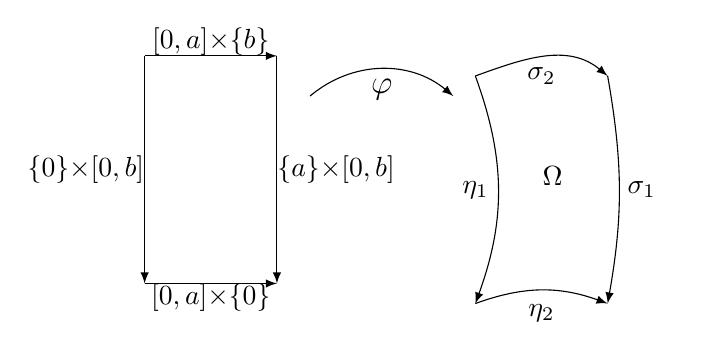
\begin{tikzpicture}[x=1.4cm,y=1.7cm]
    \pgfmathsetmacro{\L}{1.7}
    \pgfmathsetmacro{\l}{1.2}
    \pgfmathsetmacro{\d}{0.5}
    \coordinate (A) at (0,0);
    \coordinate (B) at (\l,0);
    \coordinate (C) at (0,1.7);
    \coordinate (D) at (\l,\L);
    \begin{scope}[shift={(3,-0.15)}]
    \coordinate (A2) at (0,0);
    \coordinate (B2) at (\l,0);
    \coordinate (C2) at (0,1.7);
    \coordinate (D2) at (\l,\L);
    %  \coordinate (A2) at ($(AA)$);
    %  \coordinate (B2) at ($(BB)+(120:0.3)$);
    %  \coordinate (C2) at ($(CC)+(-25:0.3)$);
    %  \coordinate (D2) at ($(BB)+(C2)-(A2)$);
    \draw[-latex] (A2) to[in=160,out=20] (B2);
    \draw[latex-] (B2) to[in=-80,out=80] (D2);
    \draw[latex-] (D2) to[in=20,out=140] (C2);
    \draw[-latex] (C2) to[in=70,out=-70] (A2);

    \draw ($(A2)!0.5!(B2)$) node[anchor=north,inner sep=0pt]{$\eta_2$};
    \draw ($(B2)!0.5!(D2)$) node[anchor=west,inner sep=7pt]{$\sigma_1$};
    \draw ($(D2)!0.5!(C2)$) node{$\sigma_2$};
    \draw ($(A2)!0.5!(C2)$) node{$\eta_1$};
    \end{scope}
    \draw[black,-latex] (A) -- (B) node[midway,anchor=north,inner sep=0pt]{$[0,a]{\times}\{0\}$};
    \draw[black,latex-] (B) -- (D) node[midway,anchor=west,inner sep=0pt]{$\{a\}{\times}[0,b]$};
    \draw[black,latex-] (D) -- (C) node[midway,anchor=south,inner sep=0pt]{$[0,a]{\times}\{b\}$};
    \draw[black,-latex] (C) -- (A) node[midway,anchor=east,inner sep=0pt]{$\{0\}{\times}[0,b]$};
    \coordinate (tmp1) at ($(D)+(0.3,-0.3)$);
    \coordinate (tmp2) at ($(3,2)+(-0.2,-0.6)$);

    \draw ($(A2)!0.5!(D2)$)++(0.1,0.1) node{$\Omega$};
    \draw[-latex] (tmp1) to[out=40,in=140] (tmp2);
    \draw ($(tmp1)!0.5!(tmp2)$)++(90:0.05) node{\large$\varphi$};

  \end{tikzpicture}
  \caption{Illustration of the notation of Lemma \ref{lem:geod-curv}} \label{fig:lem-geod}
\end{figure}
\begin{proof}
  We only prove the lemma for the curves $\eta_1$ and $\sigma_1$. The formulas for $\eta_2$ and $\sigma_2$ are obtained in a similar way. Using \eqref{eq:courb-geod-u} and the Hazzidakis formula \eqref{eq:hazz} with $u=a$ and $v=b$, we obtain
  \begin{equation*}
    \omega(a,b) = \omega(0,0) - \int_0^a\ko_{\eta_2} - \int_{-b}^0\ko_{\eta_1} - \int_{\Omega}K 
                  =\omega(a,0) - \int_{-b}^0\ko_{\eta_1} - \int_{\Omega}K,
\end{equation*}
so that
\begin{equation*}
   \int_{-b}^0\ko_{\sigma_1} = - \int_0^b\DV\omega(a,v)\dv = \int_{-b}^0\ko_{\eta_1} + \int_{\Omega}K.
  \end{equation*} 
  To prove the inequalities \eqref{eq:ineq-geod}, we first note that \eqref{eq:geod-curv-c4} implies 
  \begin{equation*}
    \int_0^a{\ko_{\eta_1}^+} - \int_0^a{\ko_{\sigma_1}^+} + \int_{\Omega}{K^+} = \int_0^a{\ko_{\eta_1}^-} - \int_0^a{\ko_{\sigma_1}^-} + \int_{\Omega}{K^-}.
  \end{equation*}
  Subdividing the curves $\eta_1$ and $\sigma_1$ according to the sign changes of $\ko_{\eta_1}$ and $\ko_{\sigma_1}$, it is possible to assume that the sign of $\ko_{\eta_1}$ and $\ko_{\sigma_1}$ is constant on $[0,a]$. The discussion is then simplified to the two following cases:
  \begin{itemize}
  \item if $\ko_{\eta_1}$ and $\ko_{\sigma_1}$ have the same sign (say, nonnegative), then
    \begin{equation*}
      \int_0^a{\ko_{\eta_1}^-}-\int_0^a{\ko_{\sigma_1}^-}+\int_{\Omega}{K^-}=\int_{\Omega}{K^-}\geq 0;
    \end{equation*}
  \item if $\ko_{\eta_1}$ and $\ko_{\sigma_1}$ have different signs (say, $\ko_{\eta_1} \geq 0$ and $\ko_{\sigma_1}\leq 0$), then
    \begin{equation*}
      \int_0^a\ko_{\eta_1}^+-\int_0^a{\ko_{\sigma_1}^+} + \int_{\Omega}{K^+} = \int_0^a{\ko_{\eta_1}^+}+\int_{\Omega}{K^+}\geq 0.
    \end{equation*}
  \end{itemize}
\end{proof}

%Let us prove the existence of a piecewise smooth Chebyshev net on $\sect$.
\begin{theorem}[Existence of piecewise smooth Chebyshev nets on sectors] \label{thm:piecewise-smooth-sector}
  Let $\sect$ be a sector delimited by the two piecewise smooth curves $\eta_1:\R^-\to\surf$ and $\eta_2:\R^+\to\surf$. We denote $\pi-\theta_1\in(0,\pi)$ the exterior angle of this sector and we suppose that $\sect$ satisfies the conditions \eqref{eq:cond-sectorb}. Then, there exist $\Npiece\geq 1$ polygons $\{\halfP^i_e\}_{1\leq i\leq \Npiece}$ such that $(\R^+)^2 = \cup_{i=1}^{\Npiece}\halfP^i_e$ and int$(\halfP^i_e)\cap$int$(\halfP_e^j)=\varnothing$ for all $i\neq j$, and Chebyshev coordinates $\varphi$ on $\sect$ such that $\eta_1$ and $\eta_2$ are coordinate curves. Moreover, the angle $\omega = \angle(\DU \varphi,\DV \varphi)$ of the net satisfies the nonsmooth Hazzidakis formula
\begin{equation}\label{eq:hazz-non-lisse}
  \omega(u,v) = \theta_1 - \tau\big(\eta_2\big|_{[0,u]}\big)
  - \tau \big(\eta_1\big|_{[-v,0]}\big) - \int_{\varphi([0,u]\Times[0,v])}K,
\end{equation}
for all $u,v\in\R^+$, and is bounded away from $0$ and $\pi$ by the positive real number
\begin{equation}\label{eq:bound-max-angles3}
\min\left(\pi-\psi-\int_\sect K^+-\tau_+(\eta_1)-\tau_+(\eta_2),~ 
\psi-\int_\sect K^- - \tau_-(\eta_1)-\tau_-(\eta_2)\right).
\end{equation}
Finally, $\varphi\big|_{\halfP^i_e}:\halfP^i_e\to\varphi(\halfP^i_e)\subset\sect$ is a diffeomorphism, for all $1\leq i\leq \Npiece$.
\end{theorem}

\begin{figure}[!htp]
  \captionsetup{justification=centering}
  \begin{center}
    \begin{subfigure}{.5\textwidth}
      \begin{center}
        \captionsetup{justification=centering}
        \begin{tikzpicture}[x=1.2cm,y=1.2cm] 
          \schem{1}
          \node[circle,draw,inner sep=0.5pt,scale=1.1] at ($(a0)!0.5!(bt3)$){$4$};
          \node[circle,draw,inner sep=0.5pt,scale=1.1] at ($(az1)!0.5!(bt4)$){$5$};
          \node[circle,draw,inner sep=0.5pt,scale=1.1] at ($(az2)!0.5!(bt5)$){$6$};
          \node[circle,draw,inner sep=0.5pt,scale=1.1] at ($(a1)!0.5!(a3)$){$1$};
          \node[circle,draw,inner sep=0.5pt,scale=1.1] at ($(a3)!0.5!(bt4)$){$2$};
          \node[circle,draw,inner sep=0.5pt,scale=1.1] at ($(bt4)!0.5!(a5)$){$3$};
        \end{tikzpicture}
        \caption{Parallel transport of $\eta_2$ along $\eta_1$\\ (case chosen for the proof)}
      \end{center}
    \end{subfigure}%
    \begin{subfigure}{.5\textwidth}
      \begin{center}
        \captionsetup{justification=centering}
        \begin{tikzpicture}[x=1.2cm,y=1.2cm] 
          \schem{1}
          \node[circle,draw,inner sep=0.5pt,scale=1.1] at ($(a0)!0.5!(bt3)$){$2$};
          \node[circle,draw,inner sep=0.5pt,scale=1.1] at ($(az1)!0.5!(bt4)$){$4$};
          \node[circle,draw,inner sep=0.5pt,scale=1.1] at ($(az2)!0.5!(bt5)$){$6$};
          \node[circle,draw,inner sep=0.5pt,scale=1.1] at ($(a1)!0.5!(a3)$){$1$};
          \node[circle,draw,inner sep=0.5pt,scale=1.1] at ($(a3)!0.5!(bt4)$){$3$};
          \node[circle,draw,inner sep=0.5pt,scale=1.1] at ($(bt4)!0.5!(a5)$){$5$};
        \end{tikzpicture}
        \caption{Parallel transport of $\eta_1$ along $\eta_2$}\label{fig:Nhalf-surface-sym}
      \end{center}
    \end{subfigure}
    \caption{Parallel transport of $\eta_1$ and $\eta_2$ along each other ($N_1=1$, $N_2=2$):\\ numbering of the double induction process}
\label{fig:scheme-pr-recursive}
  \end{center}
\end{figure}

\begin{proof}
  We first split the two curves $\eta_1$ and $\eta_2$ into smooth pieces. We denote $N_1+1\geq1$ and $N_2+1\geq1$ the number of smooth pieces of the curves $\eta_1$ and $\eta_2$, respectively. Then, we parallel transport the curve $\eta_2$ along each smooth piece of $\eta_1$. This is done recursively on $N_1$. The parallel transport of $\eta_2$ along a piece of $\eta_1$ is obtained by induction on $N_2$. Hence, we have two nested induction arguments (see Figure \ref{fig:scheme-pr-recursive}). We observe that, by symmetry, the role of the two curves can be switched, as can be seen in the same figure. Hence, we can always suppose that $N_1\geq N_2$. Once the construction is over, we prove the nonsmooth Hazzidakis formula \eqref{eq:hazz-non-lisse}. 
  \begin{proofpart}[Formulation of the first induction process (on $N_1\geq0$)]
    We suppose that $N_2\in\{0,...,N_1\}$ is a given fixed integer and we denote $(\H_{N_1+1})$ the following induction hypothesis:

  \textit{  for any sector $\sect$ of exterior angle $\pi-\theta_1\in(0,\pi)$, delimited by the two curves $\eta_1$ and $\eta_2$ having respectively $N_1+1$ and $N_2+1$ smooth pieces and satisfying \eqref{eq:cond-sectorb}, there exist polygons $\{\halfP^i_c\}_{1\leq i\leq \Npiece}$ and a Chebyshev net $\varphi: (\R^+)^2\to \sect$ such that:
    \begin{itemize}
    \item $(\R^+)^2 = \cup_{i=1}^{\Npiece}\halfP^i_e$ and int$(\halfP^i_e)\cap$int$(\halfP_e^j)=\varnothing$ for all $i\neq j$;
    \item $\eta_1$ and $\eta_2$ are coordinate curves;
    \item the angle $\omega = \angle(\DU \varphi,\DV \varphi)$ of $\varphi$ satisfies the nonsmooth Hazzidakis formula \eqref{eq:hazz-non-lisse};
    \item $\varphi\big|_{\halfP^i_e}:\halfP^i_e\to\varphi(\halfP^i_e)\subset\sect$ is a diffeomorphism, for all $i\in\{1,...,\Npiece\}$.
    \end{itemize}}
\end{proofpart}
\begin{proofpart}[Proof of the first induction process ($1^{\text{st}}$ part of the construction)]
We firstly check that $(\H_1)$ holds. Since $N_2\leq N_1$, we have $N_2=0$. Hence, the sector $\sect$ is delimited by the two smooth curves $\eta_1$ and $\eta_2$ and $(\H_1)$ holds, with $\Npiece=1$, by Proposition \ref{prop:sector}.
  Now, for $N_1\geq1$, we suppose that $(\H_{N_1})$ holds and we prove that $(\H_{N_1+1})$ also holds. Thus, we suppose that $\sect$ is delimited by two curves $\eta_1$ and $\eta_2$ having respectively $N_1+1\geq 2$ and $N_2+1\geq 1$ smooth pieces. Let
  \begin{equation*}
    -\infty = a_{1,N_1+1} < ... < a_{1,0} = 0 = a_{2,0} < ... < a_{2,N_2+1}=\infty
  \end{equation*} 
  be such that, for all $l=1,2$, $\eta_l$ restricted to $[a_{l,i-1},a_{l,i}]$ is a smooth curve, for all $i\in\{1,...,N_l+1\}$. We denote $\eta_{l,i}:[a_{l,i-1},a_{l,i}]\to\surf$ this piece of the curve $\eta_l$ and $\ko_{l,i}:[a_{l,i-1},a_{l,i}]\to\R$ its geodesic curvature.
  We denote $\psi_{l,i} = (-1)^l\angle\big(\eta_{l,i}'(a_{l,i}), \eta_{l,i+1}'(a_{l,i})\big)$ for all $i\in\{ 1,...,N_l\}$ and $l\in\{1,2\}$ (see Figure \ref{fig:pr-premiere-constr}). To abbreviate the notation, we set $\tilde\eta_{1,1} = \eta_{1,1}$. 
\end{proofpart}
\begin{proofpart}[Formulation of the second induction process (on $n\in\{1,...,N_2+1\}$)]
  We parallel transport in what follows the curve $\eta_2$ along $\eta_{1,1}$. % for an illustration of the following lemma.
See Figure \ref{fig:pr-premiere-constr} for the notation and Figure \ref{fig:Nhalf-surface-constr} for an illustration of the construction. For all $n\in\{1,...,N_2+1\}$, we denote $(\tilde\H_n)$ the following induction hypothesis:

    \textit{for all $j\in\{1,...,n\}$, let $\tilde\eta_{1,j}:[a_{1,1},0]\to\sect$ be a smooth curve intersecting $\eta_{2,j}$ at $\eta_{2,j}(a_{2,j-1}) = \tilde\eta_{1,j}(0)$. If $n>1$, for all $j\in\{1,...,n-1\}$, let $\halfP^j_e = [a_{2,j-1},a_{2,j}]\Times[0,-a_{1,1}]\subset(\R^+)^2$ and assume that $\varphi_j : \halfP^j_e\to \halfP_c^j\subset\sect$, with $\halfP^j_c = \varphi_j(\halfP^j_e)$, are Chebyshev nets such that
\begin{align*}
\varphi_j(a_{2,j-1},v) = \tilde\eta_{1,j}(-v),\quad \varphi_j(a_{2,j},v) = \tilde\eta_{1,j+1}(-v),&\quad\forall v\in [0,-a_{1,1}],\\
\qquad\varphi_j(u,0) = \eta_{2,j}(u),\qquad\qquad\qquad\qquad\qquad\qquad&\quad\forall u\in [a_{2,j-1},a_{2,j}].
\end{align*}
Then, there exists a Chebyshev net $\varphi_n:\halfP^n_e\subset(\R^+)^2\to \halfP_c^n\subset \sect$, with $\halfP^n_e = [a_{2,n-1},a_{2,n}]\Times[0,-a_{1,1}]$ and $\halfP^n_c = \varphi_n(\halfP^n_e)$. Moreover, the set $\halfP^n_c$ satisfies:
\begin{enumerate}
\item \label{it:pr-smoo-1} if $n>1$, then $\halfP_c^{n-1}\cap\halfP^n_c=\tilde\eta_{1,n}$;
\item \label{it:pr-smoo-2} if $n>2$, then $\halfP_c^j\cap\halfP^n_c=\varnothing$, for all $j\in\{1,...,n-2\}$.
\end{enumerate}
Finally, suppose that $n<N_2+1$ and denote $\tilde\eta_{1,n+1}:[a_{1,1},0]\to\sect$ the curve defined by $\tilde\eta_{1,n+1}(v) = \varphi_n(a_{2,n},-v)$ for all $v\in[a_{1,1},0]$. This curve intersects $\eta_{2,n+1}$ at $\eta_{2,n+1}(a_{2,n}) = \tilde\eta_{1,n+1}(0)$, forming an interior angle denoted $\theta_{n+1}\in[0,\pi]$. Then, $\theta_{n+1}$ and the geodesic curvature $\tilde\ko_{1,n+1}:[a_{1,1},0]\to\R$ of $\tilde\eta_{1,n+1}$ satisfy respectively
\begin{subequations}\label{eq:pr-cond-induction}
  \begin{alignat}{2}\label{eq:pr-cond-induction:1}
    \theta_{n+1} &= \theta_1-\tau(\eta_2\big|_{[0,a_{2,n}]})\in(0,\pi),\\
    \int_{-v}^0\tilde\ko_{1,n+1} &= \int_{-v}^0\ko_{1,1} + \sum_{k=1}^{n}\int_{\varphi_k([a_{2,k-1},a_{2,k}]\Times[0,v])}K,~~\forall v\in[0,-a_{1,1}]. \label{eq:pr-cond-induction:2}
  \end{alignat}
\end{subequations}}
\end{proofpart}
  \begin{figure}[!htp]
    \centering
    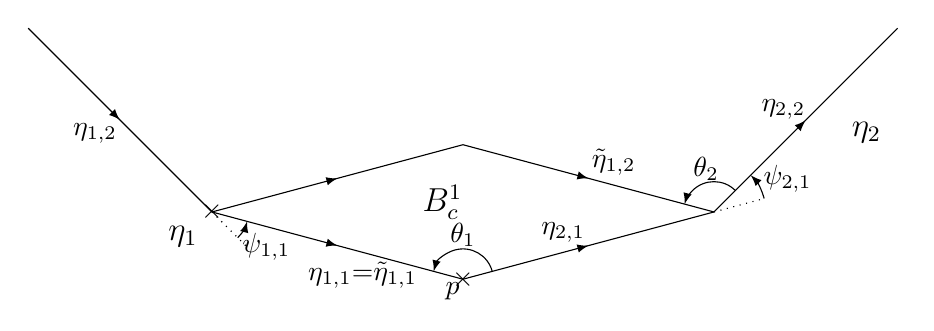
\begin{tikzpicture}[x=1.1cm,y=1.1cm]
      \begin{scope}[rotate=15]
      \pgfmathsetmacro{\RR}{0.6}
      \pgfmathsetmacro{\Rint}{0.35}

      \begin{scope}[decoration={markings,mark=at position 0.5 with {\arrow{latex}}}] 
        
        \draw[postaction={decorate}] (0,0) coordinate (a0) -- +(-60:3) coordinate[pos=0.5] (g0) coordinate (a1);
        \draw[postaction={decorate}] (a1) -- ($(a1)+(-30:3)$) coordinate[pos=0.6] (g1) coordinate (a2);
        \draw[postaction={decorate}] (a2) -- ($(a2)+(0:3)$) coordinate[pos=0.5] (g2) coordinate (a3);
        \draw[postaction={decorate}] (a3) -- ($(a3)+(30:3)$) coordinate[pos=0.5] (g3) coordinate (a4);
      \end{scope}
      \draw (g0) node[anchor=north east, inner sep=1pt]{$\eta_{1,2}$};
      \draw (g1) node[anchor=north]{$\eta_{1,1}{=}\tilde\eta_{1,1}$};
      \draw (g2) node[anchor=south east, inner sep=1pt]{$\eta_{2,1}$};
      \draw (g3) node[anchor=south east, inner sep=0pt]{$\eta_{2,2}$};
 
      % \draw[dotted] (a2) -- +(-30:\RR);
      % \draw ($(a2)+(-30:\RR)$) arc[start angle=-30,delta angle=30,radius=\RR];
      % \draw ($(a2)+(-20:\RR)$) node[anchor=west]{$\bar\psi$};
      \draw[-latex] ($(a2)+(0:\Rint)$) arc[start angle=0,delta angle=150,radius=\Rint];
      \draw ($(a2)+(75:\Rint)$) node[anchor=south,inner sep=0.5pt]{$\theta_1$};

      \draw[dotted] (a3) -- +(0:\RR);
      \draw[-latex] ($(a3)+(30:\Rint)$) arc[start angle=30,delta angle=120,radius=\Rint];
      \draw ($(a3)+(90:\Rint)$) node[anchor=south,inner sep=0.5pt]{$\theta_2$};

      \draw[-latex] ($(a3)+(0:\RR)$) arc[start angle=0,delta angle=30,radius=\RR];
      \draw ($(a3)+(25:\RR)$) node[anchor=west]{$\psi_{2,1}$};
      \draw ($(g3)+(0.3,0.2)$) node[anchor=north west, inner sep=9pt]{\large$\eta_2$};


      \begin{scope}[black,decoration={markings,mark=at position 0.5 with {\arrow{latex}}}] 
        \draw[postaction={decorate}] (a1) -- ($(a1)+(0:3)$) coordinate[pos=0.5] (gt2) coordinate (at3);
 %       \draw (gt2) node[anchor=south]{$\tilde\eta_{2,1}$};
      \end{scope}
      \begin{scope}[color=black,decoration={markings,mark=at position 0.5 with {\arrow{latex}}}] 
        \draw[postaction={decorate}] (at3) -- (a3) coordinate[pos=0.5] (gt13);
        \draw (gt13) node[anchor=south west, inner sep=1pt]{$\tilde\eta_{1,2}$};
      \end{scope}
      \draw ($(a1)!0.5!(a3)+(-0.2,0.17)$) node{\large$\halfP^1_c$};
      \draw (a1) node[anchor=north east, inner sep=5pt]{\large$\eta_1$};
      \draw (a2) node[anchor=north east, inner sep=1pt]{$p$};

      \draw (a1) node{$\times$};
      \draw (a2) node{$\times$};

      \draw[dotted] (a1) -- +(-60:\RR);
      \draw[-latex] ($(a1)+(-60:\RR*0.7)$) arc[start angle=-60,delta angle=30,radius=\RR*0.7];
      \draw ($(a1)+(-50:\RR*0.7)$) node[anchor=north west, inner sep=0pt]{$\psi_{1,1}$};


      \begin{scope}[color=red] 
%        \draw[postaction={decorate}] (a1) -- ($(a1)+(0:3)$) coordinate[pos=0.5] (gt2) coordinate (at3);
      \end{scope}
      \end{scope}
    \end{tikzpicture}
    \caption{Illustration of the parallel transport of $\eta_{2,1}$ along $\eta_{1,1}$ ($N_1=1$, $N_2=1$)}\label{fig:pr-premiere-constr}
  \end{figure}
\begin{proofpart}[Proof of the second induction process]
%  The statement, denoted $(\tilde\H_n)$, is proved by induction on $n\in\{1,...,N_2+1\}$. 
To prove that $(\tilde\H_1)$ holds, we apply Theorem \ref{thm:exist-cond-integr-c5} with the curves $\eta_{1,1}$ and $\eta_{2,1}$ of respective length $-a_{1,1}$ and $a_{2,1}$ and forming an interior angle $\theta_1\in (0,\pi)$ by hypothesis. We obtain a mapping $\varphi_1 : \halfP_e^1\subset(\R^+)^2\to \halfP_c^1\subset\surf$, with $B_e^1 = [a_{2,0},a_{2,1}]\Times[0,-a_{1,1}]$ and $\halfP_c^1=\varphi_1(\halfP^1_e)$. Then, using the same argument as the proof of Lemma \ref{lem:homeo}, we obtain that the mapping $\varphi_1$ is a Chebyshev net and that $\halfP_c^1\subset \sect$. Using Lemma \ref{lem:geod-curv}, we infer that $\tilde\eta_{1,2}$ has a geodesic curvature $\tilde\ko_{1,2}$ satisfying
  \begin{equation*}
    \int_{-v}^0\tilde\ko_{1,1} = \int_{-v}^0\ko_{1,1} + \int_{\varphi_1([0,a_{2,1}]\Times[0,v])}K,
  \end{equation*}
  for all $v\in [0,-a_{1,1}]$. Moreover, we deduce from \eqref{eq:courb-geod-u} that the interior angle $\theta_2 = \angle(\eta_{2,2}'(0), -\tilde\eta_{1,2}'(0))$ satisfies
  \begin{equation*}
    \theta_2 = \theta_1 - \int_0^{a_{2,1}}\ko_{2,1} - \psi_{2,2} = \theta_1 - \tau(\eta_2\big|_{[0,a_{2,1}]}).
  \end{equation*}
  Since hypothesis \eqref{eq:cond-sectorb} (with $\psi=\pi-\theta_1$) is satisfied by $\sect$, we obtain that $\theta_2\in(0,\pi)$. Hence, $(\tilde\H_1)$ holds.
 We now suppose that $(\tilde\H_{n-1})$ holds for $n\in\{0,...,N_2+1\}$. Let $\{\tilde\eta_{1,j}\}_{1\leq j\leq n}$ and $\{\varphi_j\}_{1\leq j\leq n-1}$ be respectively curves and Chebyshev nets as in the hypothesis of $(\tilde\H_n)$. Since $\theta_n\in(0,\pi)$, we apply Theorem \ref{thm:exist-cond-integr-c5} to the curves $\tilde\eta_{1,n}$ and $\eta_{2,n}$ to obtain a mapping $\varphi_n:\halfP^n_e\subset (\R^+)^2\to \halfP^n_c\subset\surf$, with $B_e^n=[a_{2,n-1},a_{2,n}]\Times[0,-a_{1,1}]$ and $B_c^n = \varphi_n(B_e^n)$. Using the same argument as in the proof of Lemma \ref{lem:homeo}, we obtain that $\varphi$ is a Chebyshev net, that $\halfP^n_c\subset\sect$ and that $\halfP^n_c$ satisfies the statements \ref{it:pr-smoo-1} and \ref{it:pr-smoo-2} of $(\tilde\H_n)$.

 We now suppose that $n<N_2+1$. Then, from Lemma \ref{lem:geod-curv} and from the assertion \eqref{eq:pr-cond-induction:2} of $(\tilde\H_{n-1})$, we infer that the geodesic curvature $\tilde\ko_{1,n+1}$ of $\tilde\eta_{1,n+1}$ satisfies 
    \begin{equation*}
      \int_{-v}^0\tilde\ko_{1,n+1} = \int_{-v}^0\tilde\ko_{1,n} + \int_{\varphi_n([a_{2,n-1},a_{2,n}]\Times[0,v])}K = \int_{-v}^0\ko_{1,0} + \sum_{k=1}^n\int_{\varphi_k([a_{2,k-1},a_{2,k}]\Times[0,v])}K,
    \end{equation*}
    for all $v\in [0,-a_{1,1}]$. Finally, from \eqref{eq:courb-geod-u} and from the assertion \eqref{eq:pr-cond-induction:1} of $(\tilde\H_{n-1})$, we infer that the interior angle $\theta_{n+1} = \angle(\eta_{2,n+1}'(a_{2,n}), -\tilde \eta_{1,n+1}'(0))$ satisfy
    \begin{equation*}
      \theta_{n+1} = \theta_n - \int_{a_{2,n-1}}^{a_{2,n}}\ko_{2,n} - \psi_{2,n} = \theta_1 - \tau(\eta_2\big|_{[0,a_{2,n}]}).
    \end{equation*}
    Then, using hypotheses \eqref{eq:cond-sectorb}, we obtain that $\theta_{n+1}\in (0,\pi)$. This concludes the proof of the statement $(\tilde\H_n)$.
\end{proofpart}

  \begin{figure}[!htp]
    \centering
    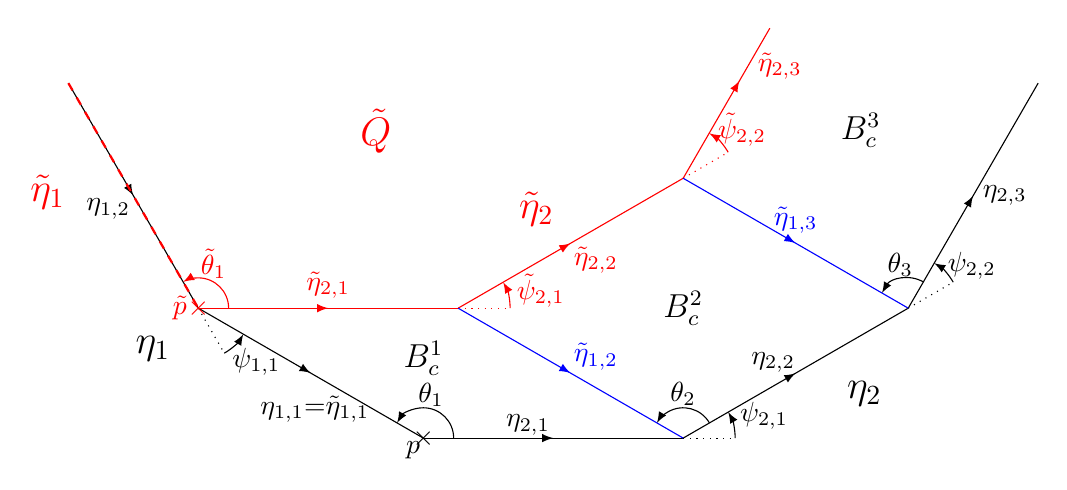
\begin{tikzpicture}[x=1.1cm,y=1.1cm]
      \pgfmathsetmacro{\RR}{0.6}
      \pgfmathsetmacro{\Rint}{0.35}

      \begin{scope}[decoration={markings,mark=at position 0.5 with {\arrow{latex}}}]         
        \draw[postaction={decorate}] (0,0) coordinate (a0) -- +(-60:3) coordinate[pos=0.5] (g0) coordinate (a1);
        \draw[postaction={decorate}] (a1) -- ($(a1)+(-30:3)$) coordinate[pos=0.6] (g1) coordinate (a2);
        \draw[postaction={decorate}] (a2) -- ($(a2)+(0:3)$) coordinate[pos=0.5] (g2) coordinate (a3);
        \draw[postaction={decorate}] (a3) -- ($(a3)+(30:3)$) coordinate[pos=0.5] (g3) coordinate (a4);
        \draw[postaction={decorate}] (a4) -- ($(a4)+(60:3)$) coordinate[pos=0.5] (g4) coordinate (a5);
      \end{scope}
      \draw (g0) node[anchor=north east, inner sep=1pt]{$\eta_{1,2}$};
      \draw[red] ($(g0)+(160:.8)$) node[anchor=north east, inner sep=1pt]{\Large$\tilde\eta_1$};
      \draw[dashed,red,thick] (a0) -- (a1);
      \draw (g1) node[anchor=north]{$\eta_{1,1}{=}\tilde\eta_{1,1}~~~~$};
      \draw (g2) node[anchor=south east, inner sep=1pt]{$\eta_{2,1}$};
      \draw (g3) node[anchor=south east, inner sep=0pt]{$\eta_{2,2}$};
      \draw (g4) node[anchor=west]{$\eta_{2,3}$};

      % \draw[dotted] (a2) -- +(-30:\RR);
      % \draw ($(a2)+(-30:\RR)$) arc[start angle=-30,delta angle=30,radius=\RR];
      % \draw ($(a2)+(-20:\RR)$) node[anchor=west]{$\bar\psi$};
      \draw[-latex] ($(a2)+(0:\Rint)$) arc[start angle=0,delta angle=150,radius=\Rint];
      \draw ($(a2)+(75:\Rint)$) node[anchor=south,inner sep=0.5pt]{$\theta_1$};

      \draw[dotted] (a3) -- +(0:\RR);
      \draw[-latex] ($(a3)+(30:\Rint)$) arc[start angle=30,delta angle=120,radius=\Rint];
      \draw ($(a3)+(90:\Rint)$) node[anchor=south,inner sep=0.5pt]{$\theta_2$};

      \draw[-latex] ($(a3)+(0:\RR)$) arc[start angle=0,delta angle=30,radius=\RR];
      \draw ($(a3)+(25:\RR)$) node[anchor=west]{$\psi_{2,1}$};
      \draw ($(g3)+(0.3,0.2)$) node[anchor=north west, inner sep=9pt]{\Large$\eta_2$};

      \draw[dotted] (a4) -- +(30:\RR);
      \draw[-latex] ($(a4)+(60:\Rint)$) arc[start angle=60,delta angle=90,radius=\Rint];
      \draw ($(a4)+(105:\Rint)$) node[anchor=south,inner sep=0.5pt]{$\theta_3$};

      \draw[-latex] ($(a4)+(30:\RR)$) arc[start angle=30,delta angle=30,radius=\RR];
      \draw ($(a4)+(55:\RR)$) node[anchor=west]{$\psi_{2,2}$};
      \begin{scope}[color=red,decoration={markings,mark=at position 0.5 with {\arrow{latex}}}] 
        \draw[postaction={decorate}] (a1) -- ($(a1)+(0:3)$) coordinate[pos=0.5] (gt2) coordinate (at3);
        \draw (gt2) node[anchor=south]{$\tilde\eta_{2,1}$};
        \draw[dotted] (at3) -- +(0:\RR);
        \draw[-latex] ($(at3)+(0:\RR)$) arc[start angle=0,delta angle=30,radius=\RR];
        \draw ($(at3)+(20:\RR)$) node[anchor=west]{$\tilde\psi_{2,1}$};
        \draw[postaction={decorate}] (at3) -- ($(at3)+(30:3)$) coordinate[pos=0.5] (gt3) coordinate (at4);
        \draw (gt3) node[anchor=north west, inner sep=1pt]{$\tilde\eta_{2,2}$};
        \draw (gt3) node[anchor=south east, inner sep=6pt]{\Large$\tilde\eta_2$};
        \draw[dotted] (at4) -- +(30:\RR);
        \draw[-latex] ($(at4)+(30:\RR)$) arc[start angle=30,delta angle=30,radius=\RR];
        \draw ($(at4)+(70:\RR)$) node[anchor=west, inner sep=6pt] {$\tilde\psi_{2,2}$};
      \end{scope}
      \begin{scope}[color=red,decoration={markings,mark=at position 0.65 with {\arrow{latex}}}] 
        \draw[postaction={decorate}] (at4) -- ($(at4)+(60:2.)$) coordinate[pos=0.75] (gt4) coordinate (at5);
      \end{scope}
      \begin{scope}[color=red,decoration={markings,mark=at position 0.5 with {\arrow{latex}}}] 
        \draw (gt4) node[anchor=west]{$\tilde\eta_{2,3}$};
      \end{scope}
      \begin{scope}[color=blue,decoration={markings,mark=at position 0.5 with {\arrow{latex}}}] 
        \draw[postaction={decorate}] (at3) -- (a3) coordinate[pos=0.5] (gt13);
        \draw (gt13) node[anchor=south west, inner sep=1pt]{$\tilde\eta_{1,2}$};
        \draw[postaction={decorate}] (at4) -- (a4) coordinate[pos=0.5] (gt14);
        \draw (gt14) node[anchor=south]{$\tilde\eta_{1,3}$};
        % \draw[postaction={decorate}] (at5) -- (a5) coordinate[pos=0.5] (gt15);
        % \draw (gt15) node[anchor=south]{$\tilde\eta_{1,6}$};
      \end{scope}
      \draw ($(a1)!0.5!(a3)+(-0.2,0.17)$) node{\large$\halfP^1_c$};
      \draw ($(at3)!0.5!(a4)$) node{\large$\halfP^2_c$};
      \draw ($(at4)!0.5!(a5)$) node{\large$\halfP^3_c$};
      \draw[color=red] ($(a0)!0.5!(at4)$) node{\Large$\tilde \sect$};
      \draw (a1) node[anchor=north east, inner sep=10pt]{\Large$\eta_1$};
      \draw (a2) node[anchor=north east, inner sep=1pt]{$p$};
      \draw[red] (a1) node[anchor=east, inner sep=4pt]{$\tilde p$};

      \draw[red] (a1) node{$\times$};
      \draw (a2) node{$\times$};

      \draw[dotted] (a1) -- +(-60:\RR);
      \draw[-latex] ($(a1)+(-60:\RR)$) arc[start angle=-60,delta angle=30,radius=\RR];
      \draw ($(a1)+(-50:\RR)$) node[anchor=north west, inner sep=0pt]{$\psi_{1,1}$};


      \begin{scope}[color=red] 
        \draw[postaction={decorate}] (a1) -- ($(a1)+(0:3)$) coordinate[pos=0.5] (gt2) coordinate (at3);
        \draw[-latex] ($(a1)+(0:\Rint)$) arc[start angle=0,delta angle=120,radius=\Rint];
        \draw ($(a1)+(60:\Rint)$) node[anchor=south, inner sep=1pt]{$\tilde\theta_1$};
      \end{scope}
    \end{tikzpicture}
    \caption{Illustration of the recursive parallel transport\\ of $\eta_2$ along $\eta_{1,1}$ ($N_1=1$, $N_2=2$)}\label{fig:Nhalf-surface-constr}
  \end{figure}
\begin{proofpart}[Proof of the first induction process ($2^{\text{nd}}$ part of the construction)]
By application of $(\tilde\H_n)$, for all $n\in\{1,...,N_2+1\}$, we obtain the existence of polygons $\{\halfP^i_e\}_{1\leq i \leq N_2+1}$ and, for all $i\in\{1,...,N_2+1\}$, of Chebyshev nets $\varphi_i : \halfP^i_e\to \halfP^i_c\subset \sect$, with $\halfP^i_c = \varphi_i(\halfP^i_e)$. Then, for all $i\in\{1,...,N_2+1\}$, we denote 
$\tilde\eta_{2,i}: [a_{2,i-1},a_{2,i}]\to\sect$ the curve defined by $\tilde\eta_{2,i}(u) = \varphi_i(u,-a_{1,1})$, for all $u\in[a_{2,i-1},a_{2,i}]$. 
We denote $\tilde\eta_2:\R^+\to \sect$ the junction of the curves $\tilde\eta_{2,i}$, with $i\in\{1,...,N_2+1\}$, defined so that 
\begin{equation*}
  \tilde\eta_2(\R^+) = \bigcup_{i=1}^{N_2+1}\tilde\eta_{2,i}([a_{2,i-1},a_{2,i}]).
\end{equation*}
We denote $\Beband = \R^+\Times[0,-a_{1,1}]$, $\Bcband = \cup_{i=1}^{N_2+1}\halfP^i_c$ and $\tilde \sect = \sect\setminus\Bcband$. Let us construct the Chebyshev net on the half-band $\Beband$. This mapping, denoted $\phiband:\Beband \to \Bcband$, is defined by
\begin{equation}\label{eq:pr-piecewise-smooth-sect3}
  \phiband(u,v) = \varphi_i(u,v), \quad\text{whenever } (u,v)\in P^i_e \text{ for $i\in\{1,...,N_2+1\}$}.
\end{equation}
Then, using that $\phiband\big|_{\halfP_e^i}$ is a diffeomorphism for all $i\in\{1,...,N_2+1\}$ and using the statements \ref{it:pr-smoo-1} and \ref{it:pr-smoo-2} of $(\tilde\H_n)$, for all $n\in\{1,...,N_2+1\}$, we obtain that the mapping $\phiband$ is a homeomorphism. We denote $\tilde\eta_1:\R^-\to\eta_1\big[(-\infty,a_{1,1}]\big]$ the curve defined by $\tilde\eta_1(t) = \eta_1(t+a_{1,1})$. Then, $\tilde \sect$ is a sector delimited by the curves $\tilde\eta_1$ and $\tilde\eta_2$ with respectively $N_1$ and $N_2+1$ smooth pieces. We now prove that $\tilde \sect$ satisfies the hypotheses of $(\H_{N_1})$ (on the interior angle and on the total curvature). First note that, using \eqref{eq:courb-geod-v}, we obtain that the interior angle $\tilde \theta_1$ of $\tilde \sect$ satisfies
\begin{equation}\label{eq:pr-piecewise-smooth-sect4}
  \tilde \theta_1 = \theta_1 - \int_{a_{1,1}}^{0}\ko_{1,1} - \psi_{1,1} = \theta_1 - \tau(\eta_1\big|_{[a_{1,1},0]}).
\end{equation}
Then, using the hypotheses \eqref{eq:cond-sectorb} on $\sect$, we obtain that $\tilde\theta_1\in (0,\pi)$. 

To simplify the notation, we use in what follows the convention that $\sum_{k=1}^{i-1}(...)=0$ when $i=1$. As parallel transport preserves the angles, we have $\tilde\psi_{2,i} = \psi_{2,i}$, for all $i\in\{1,...,N_2\}$. Therefore, from \eqref{eq:geod-curv-c4} and the definition of $\phiband$, we infer that, for all $ i\in\{1,...,N_2+1\}$ and $u\in[a_{2,i-1},a_{2,i})$,
\begin{align*}
  \tau(\tilde\eta_2\big|_{[0,u]}) &= \sum_{k=1}^{i-1}\int_{a_{2,k-1}}^{a_{2,k}}\tilde\ko_{2,k} + \int_{a_{2,i-1}}^u\tilde\ko_{2,i} + \sum_{k=1}^{i-1}\tilde\psi_{2,k}\\
  &= \sum_{k=1}^{i-1}\int_{a_{2,k-1}}^{a_{2,k}}\ko_{2,k} + \sum_{k=1}^{i-1}\int_{\halfP^k_c}K  
  + \int_{a_{2,i-1}}^u\ko_{2,i} + \int_{\varphi_i([a_{2,i-1},u]\Times[0,-a_{1,1}])}K + \sum_{k=1}^{i-1}\psi_{2,k}\\
  & =  \tau(\eta_2\big|_{[0,u]}) + \int_{\phiband([0,u]\Times[0,-a_{1,1}])} K.\snum\label{eq:pr-piecewise-smooth-sect0}
\end{align*}
Then, in the same manner as in Lemma \ref{lem:geod-curv}, we deduce from \eqref{eq:pr-piecewise-smooth-sect0} that
\begin{equation}\label{eq:pr-piecewise-smooth-sect5}
  \tau_+(\tilde\eta_2) \leq \tau_+(\eta_2)  + \int_{\Bcband} K^+ \quad\text{and}\quad\tau_-(\tilde\eta_2) \leq \tau_-(\eta_2)  + \int_{\Bcband} K^-.
\end{equation}
Moreover, we have 
\begin{equation}\label{eq:pr-piecewise-smooth-sect6}
  \tau_\pm(\tilde\eta_1) = \tau_\pm(\eta_1)-\tau_\pm(\eta_1\big|_{[a_{1,1},0]}).
\end{equation}
We now prove that $\tilde \sect$ satisfies the condition \eqref{eq:cond-sectorb1}. First, we have 
\begin{align*}
  \tau_+(\tilde\eta_1) + \tau_+(\tilde\eta_2) + \int_{\tilde \sect}K^+ + \pi-\tilde\theta_1 &\leq  \tau_+(\eta_1)-\tau_+(\eta_1\big|_{[a_{1,1},0]}) + \tau_+(\eta_2) + \int_{\Bcband}K^+\\
  &\quad+ \int_{\tilde \sect} K^+ + \pi-\theta_1 + \tau(\eta_1\big|_{[a_{1,1},0]}) \\
  &\leq \tau_+(\eta_2) + \tau_+(\eta_1) + \pi-\theta_1 + \int_\sect K^+, \snum\label{eq:pr-piecewise-smooth-sectz}
\end{align*}
using \eqref{eq:pr-piecewise-smooth-sect4}, \eqref{eq:pr-piecewise-smooth-sect5} and \eqref{eq:pr-piecewise-smooth-sect6} for the first inequality. Since hypothesis \eqref{eq:cond-sectorb1} (with $\psi=\pi-\theta_1$) is satisfied by $\sect$, we infer from \eqref{eq:pr-piecewise-smooth-sectz} that 
\begin{equation*}
  \tau_+(\tilde\eta_1) + \tau_+(\tilde\eta_2) + \int_{\tilde \sect}K^+ + \pi-\tilde\theta_1 < \pi.
\end{equation*}
Finally, we prove that $\tilde\sect$ satisfies the condition \eqref{eq:cond-sectorb2}. From \eqref{eq:pr-piecewise-smooth-sect5} and \eqref{eq:pr-piecewise-smooth-sect6}, we deduce that
\begin{equation}\label{eq:pr-piecewise-smooth-secty}
  \tau_-(\tilde\eta_1) + \tau_-(\tilde\eta_2) + \int_{\tilde \sect}K^- \leq 
  \tau_-(\eta_1) - \tau_-(\eta_1\big|_{[a_{1,1},0]}) + \tau_-(\eta_2) + \int_\sect K^-.
\end{equation}
Then, using the hypothesis \eqref{eq:cond-sectorb2} on $\sect$, we infer from \eqref{eq:pr-piecewise-smooth-secty} that
\begin{equation*}
 \tau_-(\tilde\eta_1) + \tau_-(\tilde\eta_2) + \int_{\tilde \sect}K^- < \pi-\theta_1 - \tau_-(\eta_1\big|_{[a_{1,1},0]}) .
\end{equation*}
Finally, using \eqref{eq:pr-piecewise-smooth-sect4}, we conclude that
\begin{equation*}
\tau_-(\tilde\eta_1) + \tau_-(\tilde\eta_2) + \int_{\tilde \sect}K^- \leq \pi-\tilde\theta_1-\tau(\eta_1\big|_{[a_{1,1},0]})-\tau_-(\eta_1\big|_{[a_{1,1},0]})  < \pi - \tilde\theta_1.
\end{equation*}
Hence, the hypotheses of $(\H_{N_1})$ are satisfied by $\tilde\sect$. We obtain the existence of polygons $\{\tilde{\halfP}^i_e\}_{1\leq i\leq\NpieceT}$ such that $\text{int}(\tilde{\halfP}^i_e)\cap\text{int}(\tilde{\halfP}^j_e)=\varnothing$ for all $i\neq j$ and $\cup_{i=1}^{\tilde\N_{\text{piece}}}\tilde \halfP^i_e = (\R^+)^2$, and a Chebyshev parametrization of $\tilde\sect$ denoted $\tilde\varphi:(\R^+)^2\to\tilde\sect$. The translation of each polygon $\tilde\halfP_e^i$ by the vector $(0,-a_{1,1})$, i.e., the set $\{\tilde \halfP^i_e + (0,-a_{1,1})\}_{1\leq i\leq \NpieceT}$ is then joined to the set $\{\halfP^i_e\}_{1\leq i\leq N_2+1}$ to obtain $\{\halfP^i_e\}_{1\leq i\leq \Npiece}$.  Moreover, we define the mapping $\varphi:(\R^+)^2\to \sect$ by
\begin{equation*}
  \varphi(u,v) = 
  \begin{cases}
    \phiband(u,v),&\text{if }(u,v)\in\Beband,\\ 
    \tilde\varphi(u,v+a_{1,1}),&\text{otherwise}.
  \end{cases}
\end{equation*}
We can show, in the same manner as for $\phiband$, that $\varphi$ is a homeomorphism.
\end{proofpart}

\begin{proofpart}[Proof of the first induction process (nonsmooth Hazzidakis formula)]
  Let $(u, v)\in (\R^+)^2$. First, we suppose that $(u, v)\in \Beband$, so that $(u, v)\in \halfP^j_e$ for some $j\in \{1,...,N_2+1\}$. By the Hazzidakis formula in the smooth setting \eqref{eq:hazz}, the angle $\omega_j$ between the parameter curves of $\varphi_j$ satisfies
\begin{equation}\label{eq:pr-piecewise-smooth-sectx}
  \omega_j(u,v) = \theta_j - \int_{a_{2,j-1}}^u\ko_{2,j} - \int_{-v}^0 \tilde\ko_{1,j} - \int_{\varphi_j([a_{2,j-1},u]\Times[0,v])}K.
\end{equation}
Then, from \eqref{eq:pr-cond-induction} and \eqref{eq:pr-piecewise-smooth-sectx}, we infer that
\begin{align*}
  \omega(u,v) = \omega_j(u,v) &= \theta_1 - \tau(\eta_2\big|_{[0,u]}) - \tau(\eta_1\big|_{[-v,0]})  - \sum_{k=1}^{j-1}\int_{\varphi_k([a_{2,k-1},a_{2,k}]\Times[0,v])}K 
  \\
  &\quad- \int_{\varphi_j([a_{2,j-1},u]\Times[0,v])}K\\
  &= \theta_1 - \tau(\eta_1\big|_{[-v,0]}) - \tau(\eta_2\big|_{[0,u]})  - \int_{\varphi([0,u]\Times[0,v])}K.
\end{align*}
We now suppose that $(u,v)\notin \Beband$ and we denote $\bar u= u$ and $\bar v=v+a_{1,1}$. Then, $\bar u, \bar v\in\R^+$ and, by $(\H_{N_1})$,  the nonsmooth Hazzidakis formula \eqref{eq:hazz-non-lisse} is satisfied by the angle $\tilde\omega$ between the coordinate curves of $\tilde\varphi$. Hence, using \eqref{eq:hazz-non-lisse} on $\tilde\omega$ and \eqref{eq:pr-piecewise-smooth-sect0}, we obtain that
\begin{align*}
  \omega(u,v) = \tilde\omega(\bar u,\bar v) &= \tilde \theta_1 - \tau(\tilde \eta_1\big|_{[-\bar v,0]}) - \tau(\tilde\eta_2\big|_{[0,\bar u]})  - \int_{\tilde\varphi([0,\bar u]\Times[0,\bar v])}K,  \\
  &= \theta_1 - \tau(\eta_1\big|_{[a_{1,1},0]}) - \tau(\eta_1\big|_{[-v,a_{1,1}]}) - \tau(\eta_2\big|_{[0,u]})\\
  &\quad- \int_{\varphi([0,u]\Times[0,-a_{1,1}])}K - \int_{\varphi([0,u]\Times[-a_{1,1},v])}K\\
  &= \theta_1 - \tau(\eta_1\big|_{[-v,0]}) - \tau(\eta_2\big|_{[0,u]}) - \int_{\varphi([0,u]\Times[0,v])}K.
\end{align*}
Hence, $(\H_{N_1+1}$) holds. This concludes the proof.
\end{proofpart}
\end{proof}
\begin{remarkE}[Explicit value of $\Npiece$]
  We easily see from the proof that $\Npiece = (N_1+1)(N_2+1)$, where $N_1+1$ and $N_2+1$ are respectively the number of smooth pieces of $\eta_1$ and $\eta_2$.
\end{remarkE}

\begin{corollaryE}[Existence of piecewise smooth Chebyshev nets on $N$-half-surfaces] \label{cor:cheb-half-surface-smooth2}
  Let $N\geq 1$ and let $\halfP_c$ be a $N$-half-surface delimited by the curves $\{\gamma_c^i\}_{1\leq i\leq N+1}$. We suppose that $\halfP_c$ satisfies the conditions
  \begin{align*}
    \tau_+(\partial \halfP_c) + \int_{\halfP_c} K^+ &< \pi,  \\
    \tau_-(\partial \halfP_c) + \int_{\halfP_c} K^-  &< \psim. 
  \end{align*}
  Then, there exist $\Npiece\geq 1$ polygons $\{\halfP^i_e\}_{1\leq i\leq \Npiece}$ such that $(\R^+)^2 = \cup_{i=1}^{\Npiece}\halfP^i_e$ and $\text{int}(\halfP_e^i)\cap\text{int}(\halfP_e^j)=\varnothing$ for all $i\neq j$, and Chebyshev coordinates $\varphi$ on $\halfP_c$ such that $\{\gamma^i_c\}_{1\leq i\leq N+1}$ are coordinate curves. Moreover, the angle $\omega = \angle(\DU \varphi,\DV \varphi)$ of the net is bounded away from $0$ and $\pi$ by the positive real number
\begin{equation*}
\varepsilon=\min\left(\pi-\tau_+(\partial \halfP_c)-\int_{\halfP_c} K^+,\quad\psim-\tau_-(\partial \halfP_c) - \int_{\halfP_c} K^-\right).
\end{equation*}
Finally, the mapping $\varphi\big|_{\halfP^i_e}:\halfP^i_e\to\halfP^i_c\subset\halfP_c$, with $\halfP^i_c = \varphi(\halfP^i_e)$, is a diffeomorphism, for all $i\in\{1,...,\Npiece\}$.
\end{corollaryE}
\begin{proof}
  The proof follows by combining Theorem \ref{thm:piecewise-smooth-sector} and Proposition \ref{prop:half-surface-to-sector}.
\end{proof}
%Finally, in the specific case of geodesic split half-surfaces, we have:
\begin{theorem}[Existence of piecewise smooth Chebyshev nets on geodesic $N$-half-surfaces] \label{thm:cheb-half-surface-smooth3}
  Let $N\geq 1$ and let $\halfP_c$ be a geodesic $N$-half-surface delimited by the geodesic curves $\{\gamma_c^i\}_{1\leq i\leq N+1}$. We suppose that $\halfP_c$ satisfies the conditions   
% \begin{subequations} \label{eq:cond-half-surfaceb}
%     \begin{alignat}{2}\label{eq:cond-half-surfaceb1}
%       \int_{\halfP_c} K^+ &< \pi-\psitot,\\
%       \int_{\halfP_c} K^- &<  \psim.\label{eq:cond-half-surfaceb2}
%     \end{alignat}
%   \end{subequations}
\begin{align*} 
      \int_{\halfP_c} K^+ &< \pi-\psitot,\\
      \int_{\halfP_c} K^- &<  \psim.
\end{align*}
  Then, there exist $\Npiece\geq 1$ polygons $\{\halfP^i_e\}_{1\leq i\leq \Npiece}$ such that $(\R^+)^2 = \cup_{i=1}^{\Npiece}\halfP^i_e$ and $\text{int}(\halfP_e^i)\cap\text{int}(\halfP_e^j)=\varnothing$ for all $i\neq j$, and Chebyshev coordinates $\varphi$ on $\halfP_c$ such that $\{\gamma^i_c\}_{1\leq i\leq N+1}$ are coordinate curves. Moreover, the angle $\omega = \angle(\DU \varphi,\DV \varphi)$ of the net is bounded away from $0$ and $\pi$ by the positive real number
  \begin{equation*}
    \min\left(\pi-\psitot-\int_{\halfP_c} K^+,|\psi|_{l^\infty}-\int_{\halfP_c} K^-\right).
  \end{equation*}
  Finally, the mapping $\varphi\big|_{\halfP^i_e}:\halfP^i_e\to\halfP^i_c\subset\halfP_c$, with $\halfP^i_c = \varphi(\halfP^i_e)$, is a diffeomorphism, for all $i\in\{1,...,\Npiece\}$.
\end{theorem}

 

\bibliography{references}

\end{document}
